\documentclass{beamer}
\usepackage{graphicx} % Package for images
\usepackage{caption} % Package for numbering figures
\setbeamertemplate{caption}[numbered] % Enable numbering for figures
\captionsetup{font=tiny} % Reduce caption size
\usepackage{tikz}
\usepackage{pgfplots}
\usepackage{multicol}
\usepackage{amsmath}
\usetikzlibrary{trees, positioning}
% Theme choice
\usetheme{Frankfurt} % Changed theme to Frankfurt
\pgfplotsset{compat=1.18}
\usepackage{helvet} \renewcommand{\familydefault}{\sfdefault}
\setbeamertemplate{headline}{\leavevmode\hbox{}} 

% Title and author details
\title{Image Inpainting}
\author{Dwaipayan Haldar \protect\linebreak BEE-IV, 002110801187 \protect\linebreak Dept. of Electrical Engineering \protect\linebreak Jadavpur University}
\date{4th April 2025}

\begin{document}

% Title slide
\begin{frame}
    \titlepage
\end{frame}

% Table of contents
\begin{frame}{Outline}
    \tableofcontents
\end{frame}

% Section 1
\section{Introduction}

\begin{frame}{}
    \centering
    \Huge{Introduction}
\end{frame}

\begin{frame}{What is Image Inpainting?}
     Image inpainting originated from an ancient technique performed
 by artists to restore damaged paintings or photographs with small
 defects such as scratches, cracks, dust and spots to maintain its quality
 to as close to the original as possible.
    \begin{figure}[h]
        \centering
        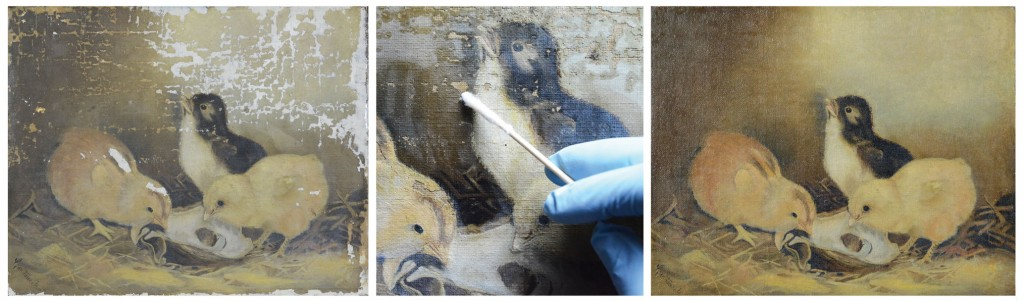
\includegraphics[width=0.7\textwidth]{ArtResto-1024x301.jpg} % Replace with your image file name
        \caption{ Hand inpainting performed by an artist. Image courtesy of Thottam (2015).}
    \end{figure}
\end{frame}

\begin{frame}{Object Removal}
     Image inpainting removes unwanted objects by filling the gaps with realistic textures using deep learning (GANs, diffusion models) or traditional methods, ensuring seamless restoration.
    \begin{figure}[h]
        \centering
        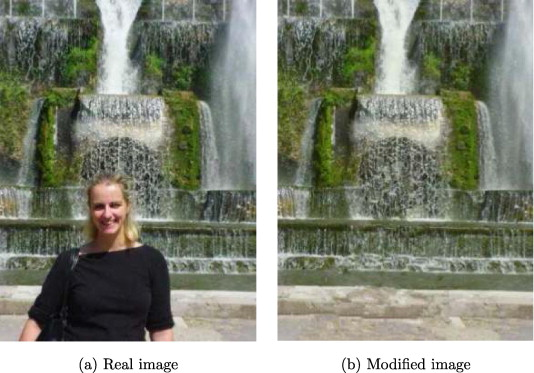
\includegraphics[width=0.6\textwidth]{Object Removal.jpg} % Replace with your image file name
        \caption{ An example of a people removal method where the person has been manually selected in the real image (a), and then automatically removed in the second image (b) by filling the region concerning the person using an exemplar-based image inpainting method. Reprinted from Criminisi et al. (2004).}
    \end{figure}
\end{frame}

\begin{frame}{Example Problem}
    \begin{figure}[h]
        \centering
        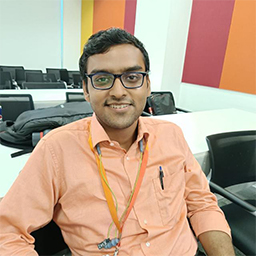
\includegraphics[width=0.6\textwidth]{Image.jpg} % Replace with your image file name
        \caption{Photo of Dwaipayan Haldar}
    \end{figure}
\end{frame}

\begin{frame}{Example Problem}
    \begin{figure}[h]
        \centering
        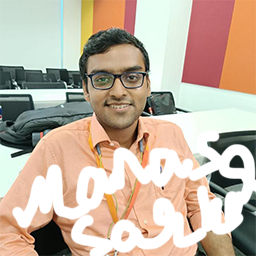
\includegraphics[width=0.6\textwidth]{Image_for_ts_gpt.png} % Replace with your image file name
        \caption{Photo of Dwaipayan Haldar distorted by Manas Sarkar}
    \end{figure}
\end{frame}

\begin{frame}{Example Problem}
    \begin{figure}[h]
        \centering
        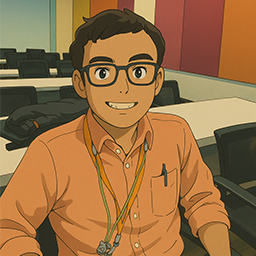
\includegraphics[width=0.6\textwidth]{Image_ghibli.jpg} % Replace with your image file name
        \caption{Ghibli of Dwaipayan Haldar}
    \end{figure}
\end{frame}

\begin{frame}{Example Problem}
    \begin{figure}[h]
        \centering
        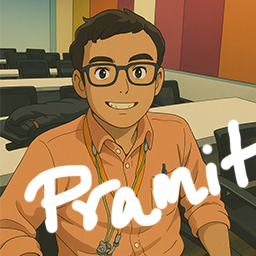
\includegraphics[width=0.6\textwidth]{Image_ghibli_Pramit.png} % Replace with your image file name
        \caption{Ghibli of Dwaipayan Haldar distorted by Pramit Khamrui}
    \end{figure}
\end{frame}

% Section 2
\section{Classification}

\begin{frame}{}
    \centering
    \Huge{Classification}
\end{frame}

\begin{frame}{Classification of different Inpainting Techniques}

\begin{center}
\begin{figure}[h!]
    \centering
    \resizebox{0.5\textwidth}{!}{%  Scale to 70% of text width
        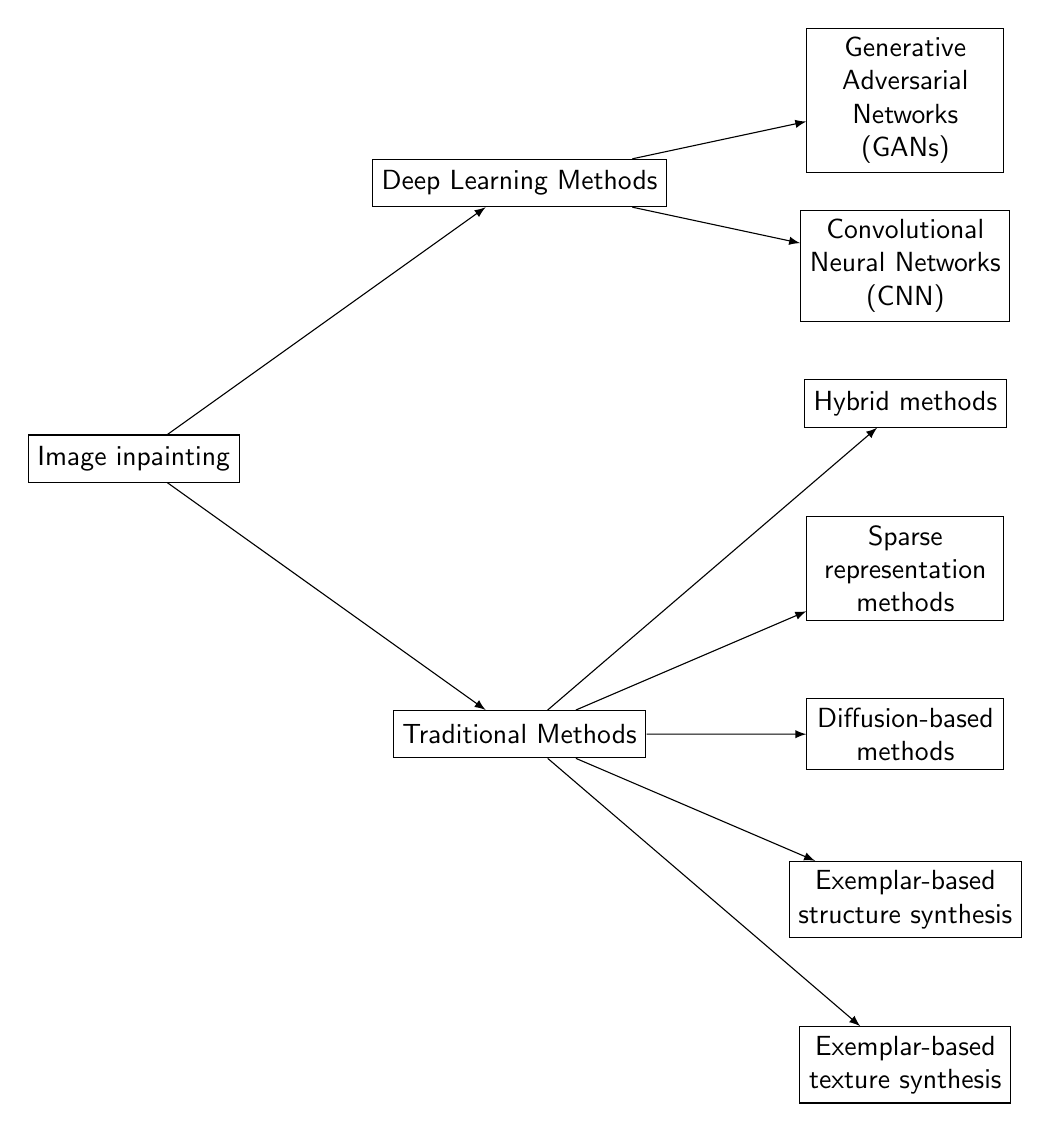
\begin{tikzpicture}[
        scale = 0.7, 
          rotate=90,  % Rotate the whole diagram 90 degrees
          level 1/.style={sibling distance=10cm}, % Adjust for new orientation
          level 2/.style={sibling distance=3cm},  % Adjust for new orientation
          level distance=7cm,                   % Adjust for new orientation
          every node/.style={rectangle, draw, align=center, minimum width=2.5cm, minimum height=0.6cm}, % Adjust node sizes
          edge from parent/.style={draw, -latex}
        ]
        \node {Image inpainting}
          child {node {Traditional Methods}
            child {node {Exemplar-based \\ texture synthesis}}
            child {node {Exemplar-based \\ structure synthesis}}
            child {node {Diffusion-based \\ methods}}
            child {node {Sparse \\ representation \\ methods}}
            child {node {Hybrid methods}}
          }
          child {node {Deep Learning Methods}
            child {node {Convolutional \\ Neural Networks \\ (CNN)}}
            child {node {Generative \\ Adversarial \\ Networks \\ (GANs)}}
          };
        \end{tikzpicture}
    }
    \caption{Hierarchical representation of image inpainting techniques in two main
 categories} % Optional caption
    \label{fig:inpainting_tree} % Optional label for referencing
\end{figure}
\end{center}

\end{frame}


\begin{frame}{Classification of different Inpainting Techniques}

\begin{center}
\begin{figure}[h!]
    \centering
    \resizebox{0.5\textwidth}{!}{% Scale to 50% of text width
        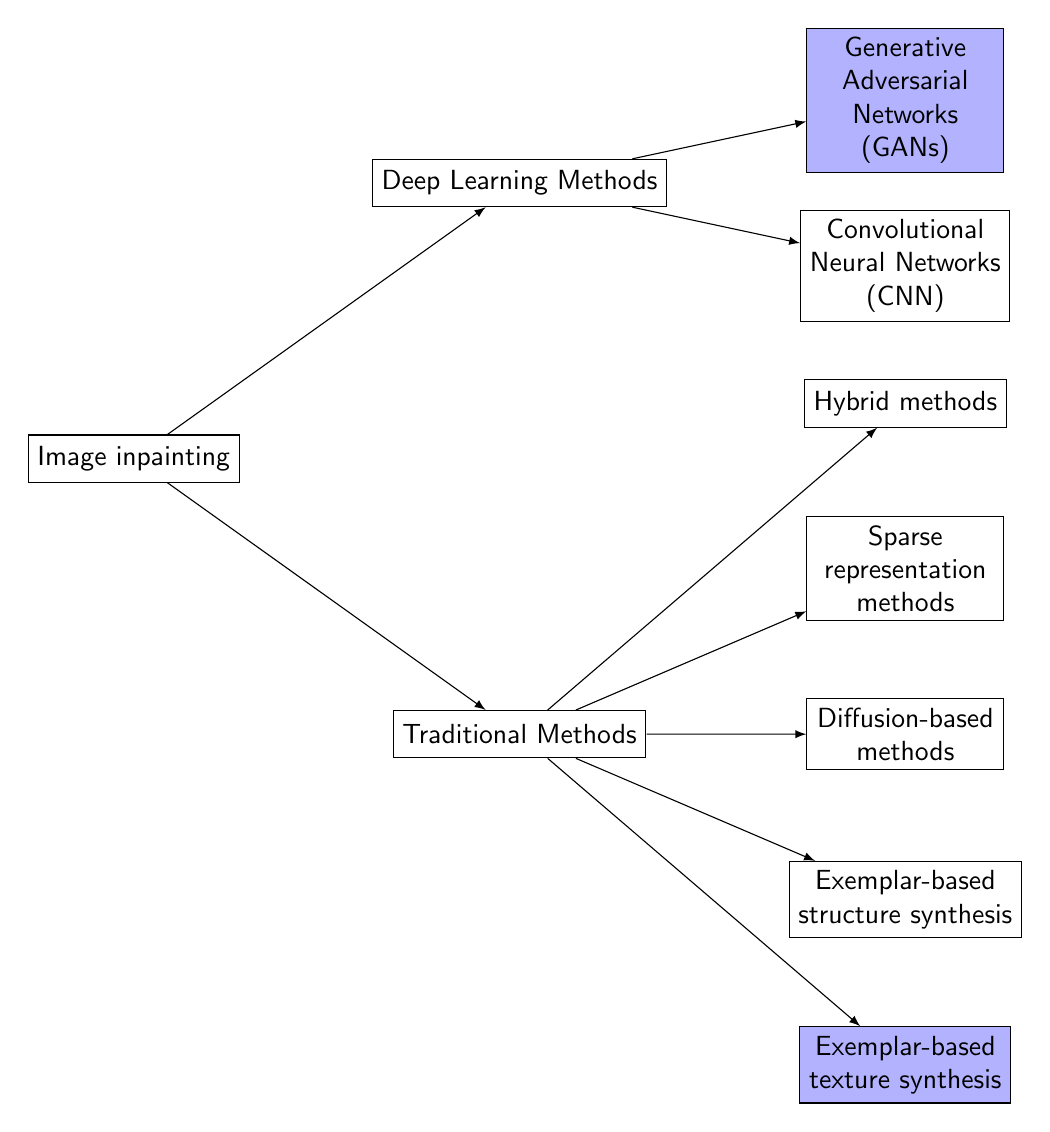
\begin{tikzpicture}[
          scale=0.7, 
          rotate=90,  % Rotate the whole diagram 90 degrees
          level 1/.style={sibling distance=10cm}, % Adjust for new orientation
          level 2/.style={sibling distance=3cm},  % Adjust for new orientation
          level distance=7cm,                   % Adjust for new orientation
          every node/.style={rectangle, draw, align=center, minimum width=2.5cm, minimum height=0.6cm}, % Adjust node sizes
          edge from parent/.style={draw, -latex}
        ]
        \node {Image inpainting}
          child {node {Traditional Methods}
            child {node [fill=blue!30] {Exemplar-based \\ texture synthesis}} % Highlighted in yellow
            child {node {Exemplar-based \\ structure synthesis}}
            child {node {Diffusion-based \\ methods}}
            child {node {Sparse \\ representation \\ methods}}
            child {node {Hybrid methods}}
          }
          child {node {Deep Learning Methods}
            child {node {Convolutional \\ Neural Networks \\ (CNN)}}
            child {node [fill=blue!30] {Generative \\ Adversarial \\ Networks \\ (GANs)}} % Highlighted in blue
          };
        \end{tikzpicture}
    }
    \caption{Hierarchical representation of image inpainting techniques in two main categories}
    \label{fig:inpainting_tree}
\end{figure}
\end{center}

\end{frame}

% Section 3
\section{Exemplar based Texture Synthesis}


\begin{frame}{}
    \centering
    \Huge{Exemplar Based Texture Synthesis}
\end{frame}


\begin{frame}{Definitions}
    \begin{block}{What is a texture?}
         A texture is a visual pattern on an infinite 2-D plane with a stationary distribution at some scale (Efros and Leung, 1999). This pattern refers to the feel (smooth, rough) of the image surface.   
    \end{block}

    \begin{block}{Types of textures}
         Textures have been traditionally classified as either regular (consisting of repeated texels) or stochastic (without explicit texels). However, almost all real-world textures lie somewhere in between these two extremes and should be captured with a single model.
    \end{block}
\end{frame}

\begin{frame}{Assumptions}
    
    \begin{block}{Assumptions}
    \begin{itemize}
        \item \textbf{Markov Random Field (MRF) Model:}The algorithm assumes that texture can be modeled as a Markov Random Field. This means that the probability distribution of a pixel's brightness value, given the brightness values of its spatial neighborhood, is independent of the rest of the image. In simpler terms, a pixel's value depends only on its neighbors.
        \item  \textbf{Stationary Texture:} The usual assumption, which this paper also makes, is that the sample texture is large enough to capture the stationarity of the texture. "Stationarity" in this context means that the statistical properties of the texture are consistent across the image.
    \end{itemize}
        
        
    \end{block}
\end{frame}

% Adding an image
\begin{frame}{Overview of Algorithm}
    \begin{itemize}
    \item Let \( I \) be an image being synthesized from a texture sample image \( I_{smp} \), where \( I_{real} \) is the real infinite texture.
    \item Let \( p \in I \) be a pixel, and \( \omega(p) \subset I \) be a square image patch of width \( w \) centered at \( p \).
    \item Let \( d(\omega_1, \omega_2) \) denote some perceptual distance between two patches.
    \item Assume all pixels in \( I \) except \( p \) are known.
    \item Based on the MRF model, assume that \( p \) is independent of \( I \setminus \omega(p) \) given \( \omega(p) \).
    \begin{figure}[h]
        \centering
        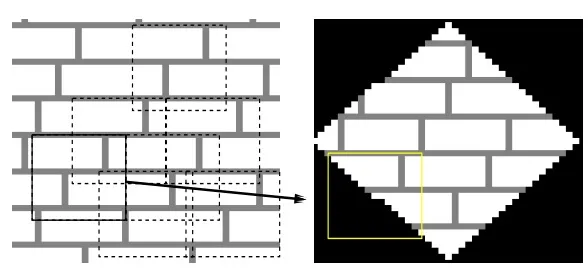
\includegraphics[width=0.5\textwidth]{Paper picture.png} % Replace with your image file name
        \caption{Algorithm Overview}
    \end{figure}
    
\end{itemize}

\end{frame}

\begin{frame}{Overview of the algorithm}
    \begin{itemize}
    
    \item Define the set:
          \[
          S(p) = \{\omega' \subset I_{real} : d(\omega', \omega(p)) = 0\}
          \]
          containing all occurrences of \( \omega(p) \) in \( I_{real} \).
          
        \item Estimate the conditional probability density function (pdf) of \( p \) using a histogram of all center pixel values in \( S(p) \).
    \item Since only a finite sample \( I_{smp} \) is available, there may not be exact matches for \( \omega(p) \).
    \item Use a heuristic to find a plausible subset \( S_0(p) \subset S(p) \) for sampling.
    \item Implement a nearest neighbor technique: find the best match \( \omega_{best} = \arg\min_{\omega} d(\omega(p), \omega) \) in \( I_{smp} \).
   
    \end{itemize}
    
\end{frame}

\begin{frame}{Overview of the algorithm}
    \begin{itemize}
         \item Include all patches \( \omega \) satisfying:
          \[
          d(\omega(p), \omega) < (1 + \epsilon) d(\omega(p), \omega_{best})
          \]
          where \( \epsilon = 0.1 \).
    \item Use the center pixel values of patches in \( S_0(p) \) to construct a histogram for \( p \).
    \item Sample from this histogram, either uniformly or weighted by \( d \).
    \item Define a suitable distance metric \( d \), such as normalized sum of squared differences (SSD) with Gaussian kernel.
    \[
    d_{ssd} \cdot G =  \frac{\sum_{i,j} G(i,j) \cdot (F_{i,j} - I_{i,j})^2}{\sqrt{\sum_{i,j} F_{i,j}^2 \cdot \sum_{i,j} I_{i,j}^2}}
    \]
    \end{itemize}
    
\end{frame}
% Adding a table
\begin{frame}{Hole filling with Texture Synthesis}
    \begin{figure}[h]
        \centering
        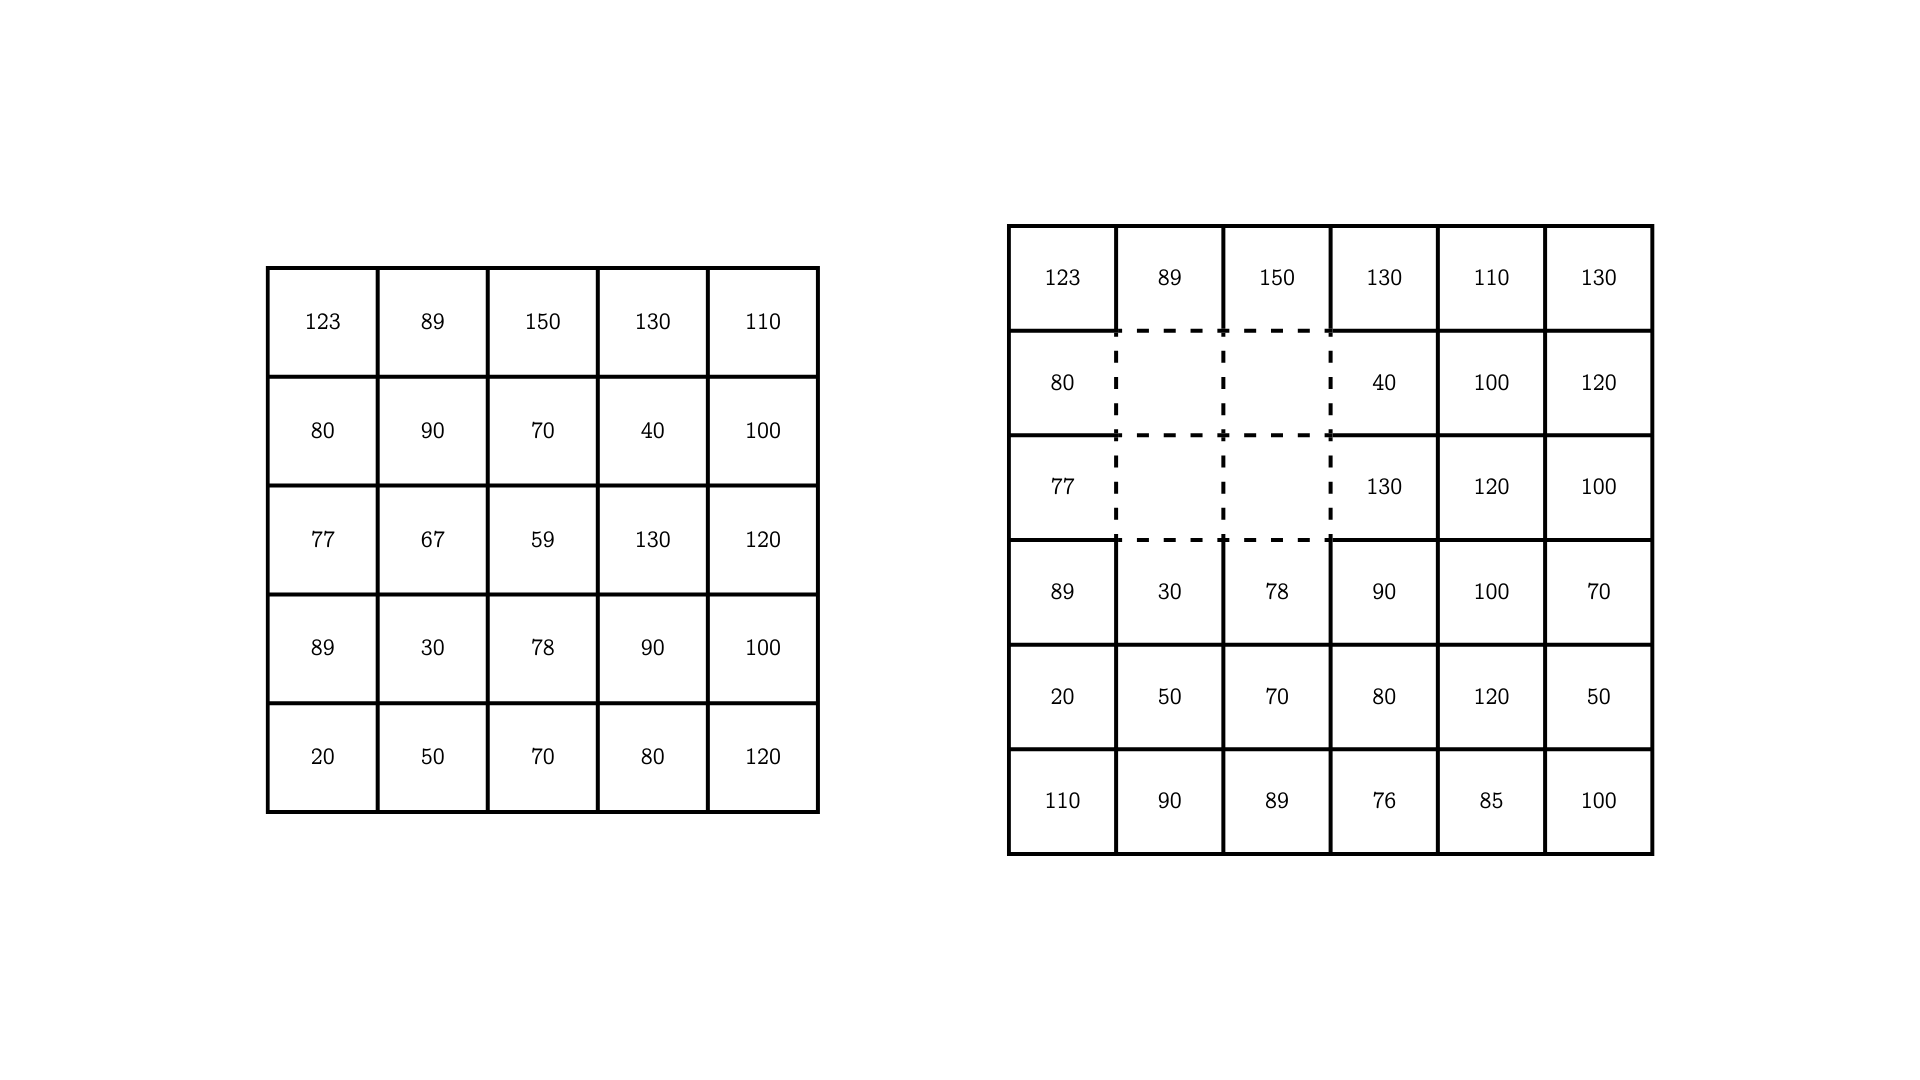
\includegraphics[width=1\textwidth]{1.png}
        \captionsetup{labelformat=empty}
    \end{figure}
\end{frame}

\begin{frame}{Hole filling with Texture Synthesis}
    \begin{figure}[h]
        \centering
        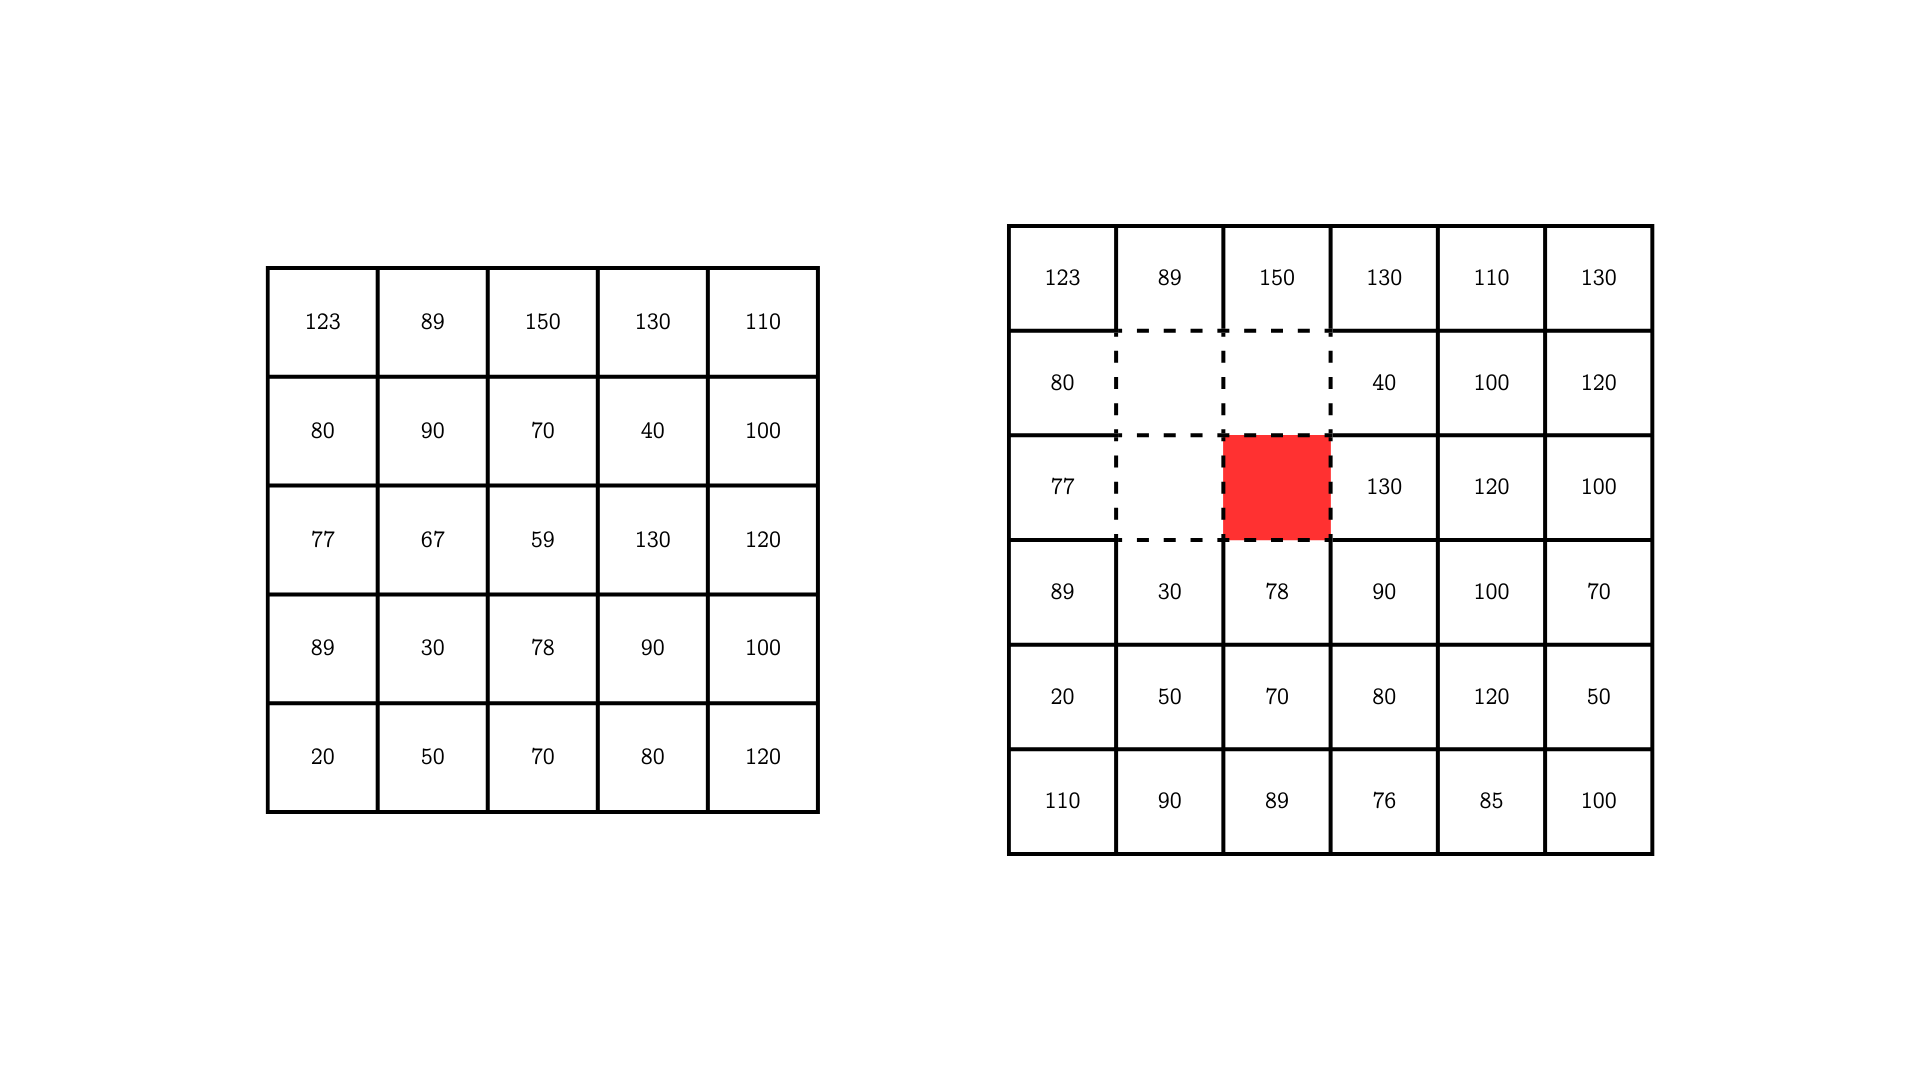
\includegraphics[width=1\textwidth]{2.png} % Replace with your image file name
        \captionsetup{labelformat=empty}
    \end{figure}
\end{frame}

\begin{frame}{Hole filling with Texture Synthesis}
    \begin{figure}[h]
        \centering
        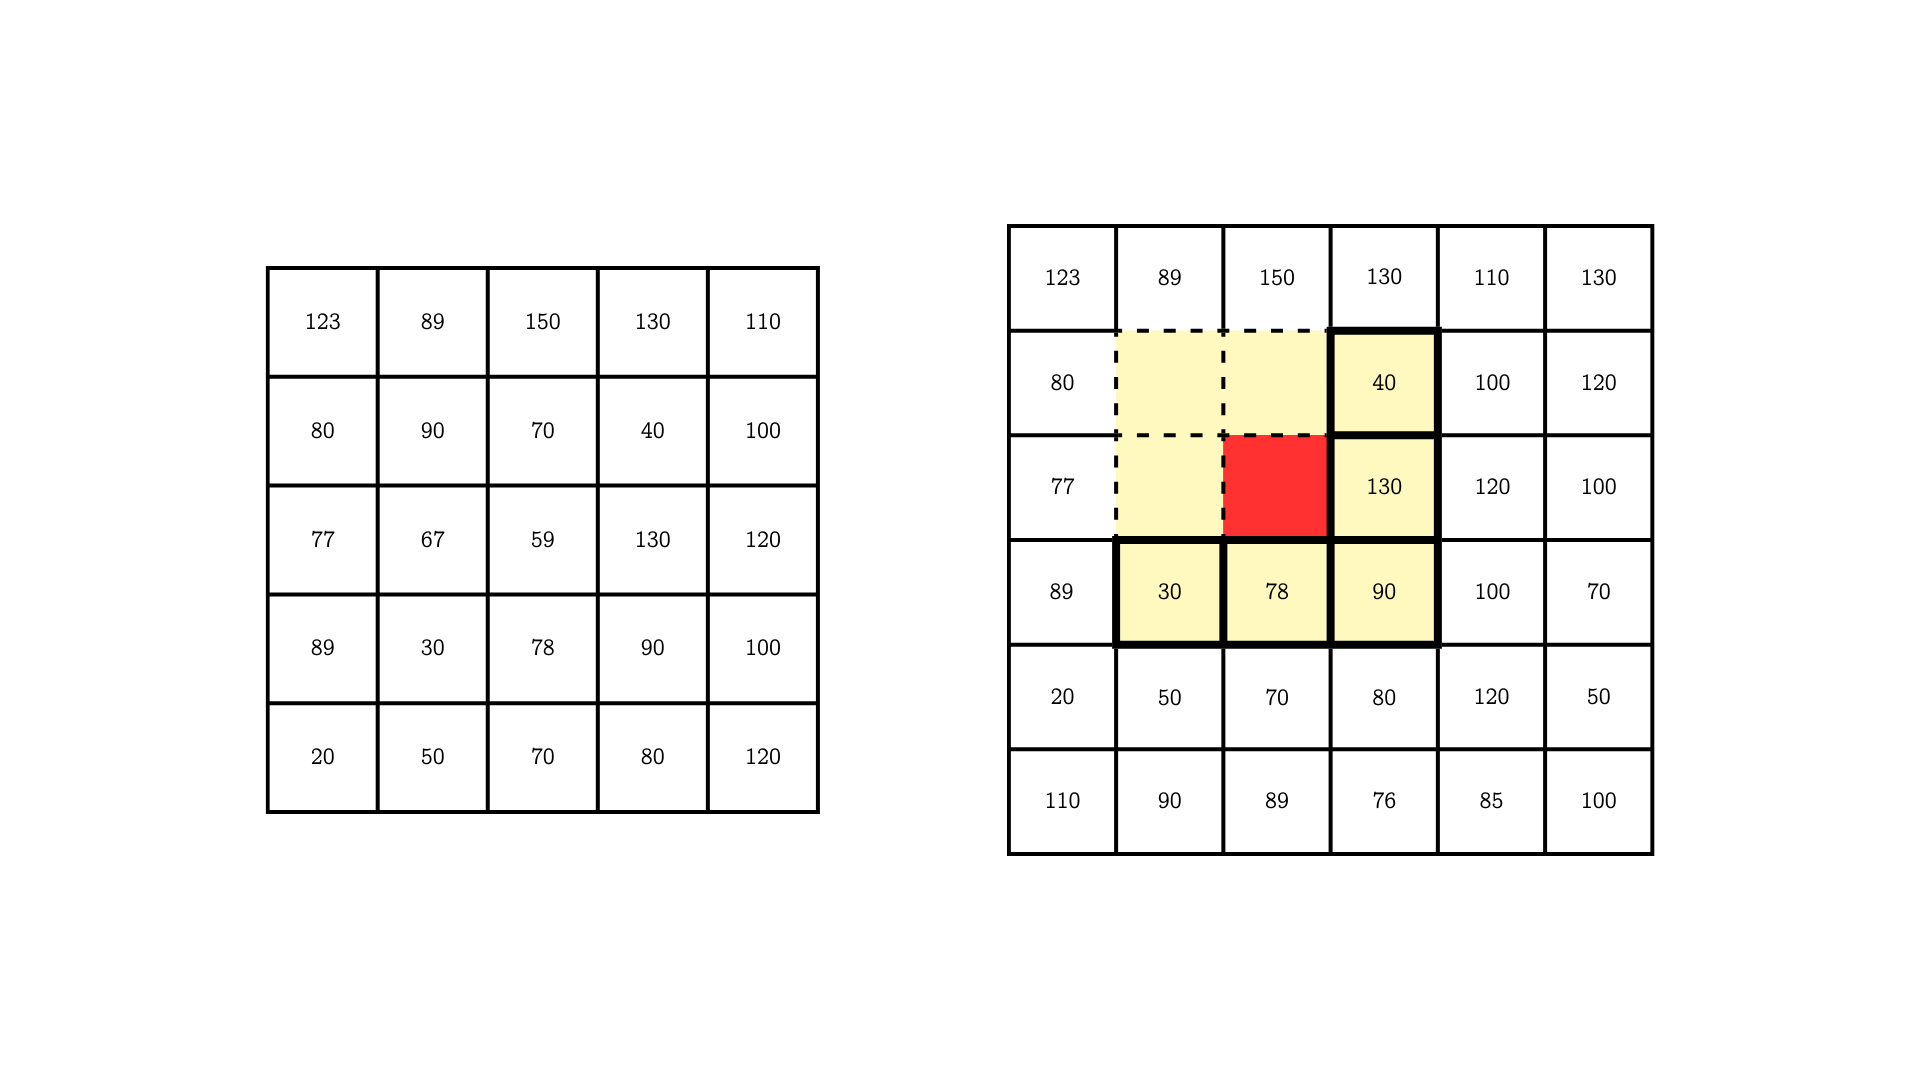
\includegraphics[width=1\textwidth]{3.png} % Replace with your image file name
        \captionsetup{labelformat=empty}
    \end{figure}
\end{frame}

\begin{frame}{Hole filling with Texture Synthesis}
    \begin{figure}[h]
        \centering
        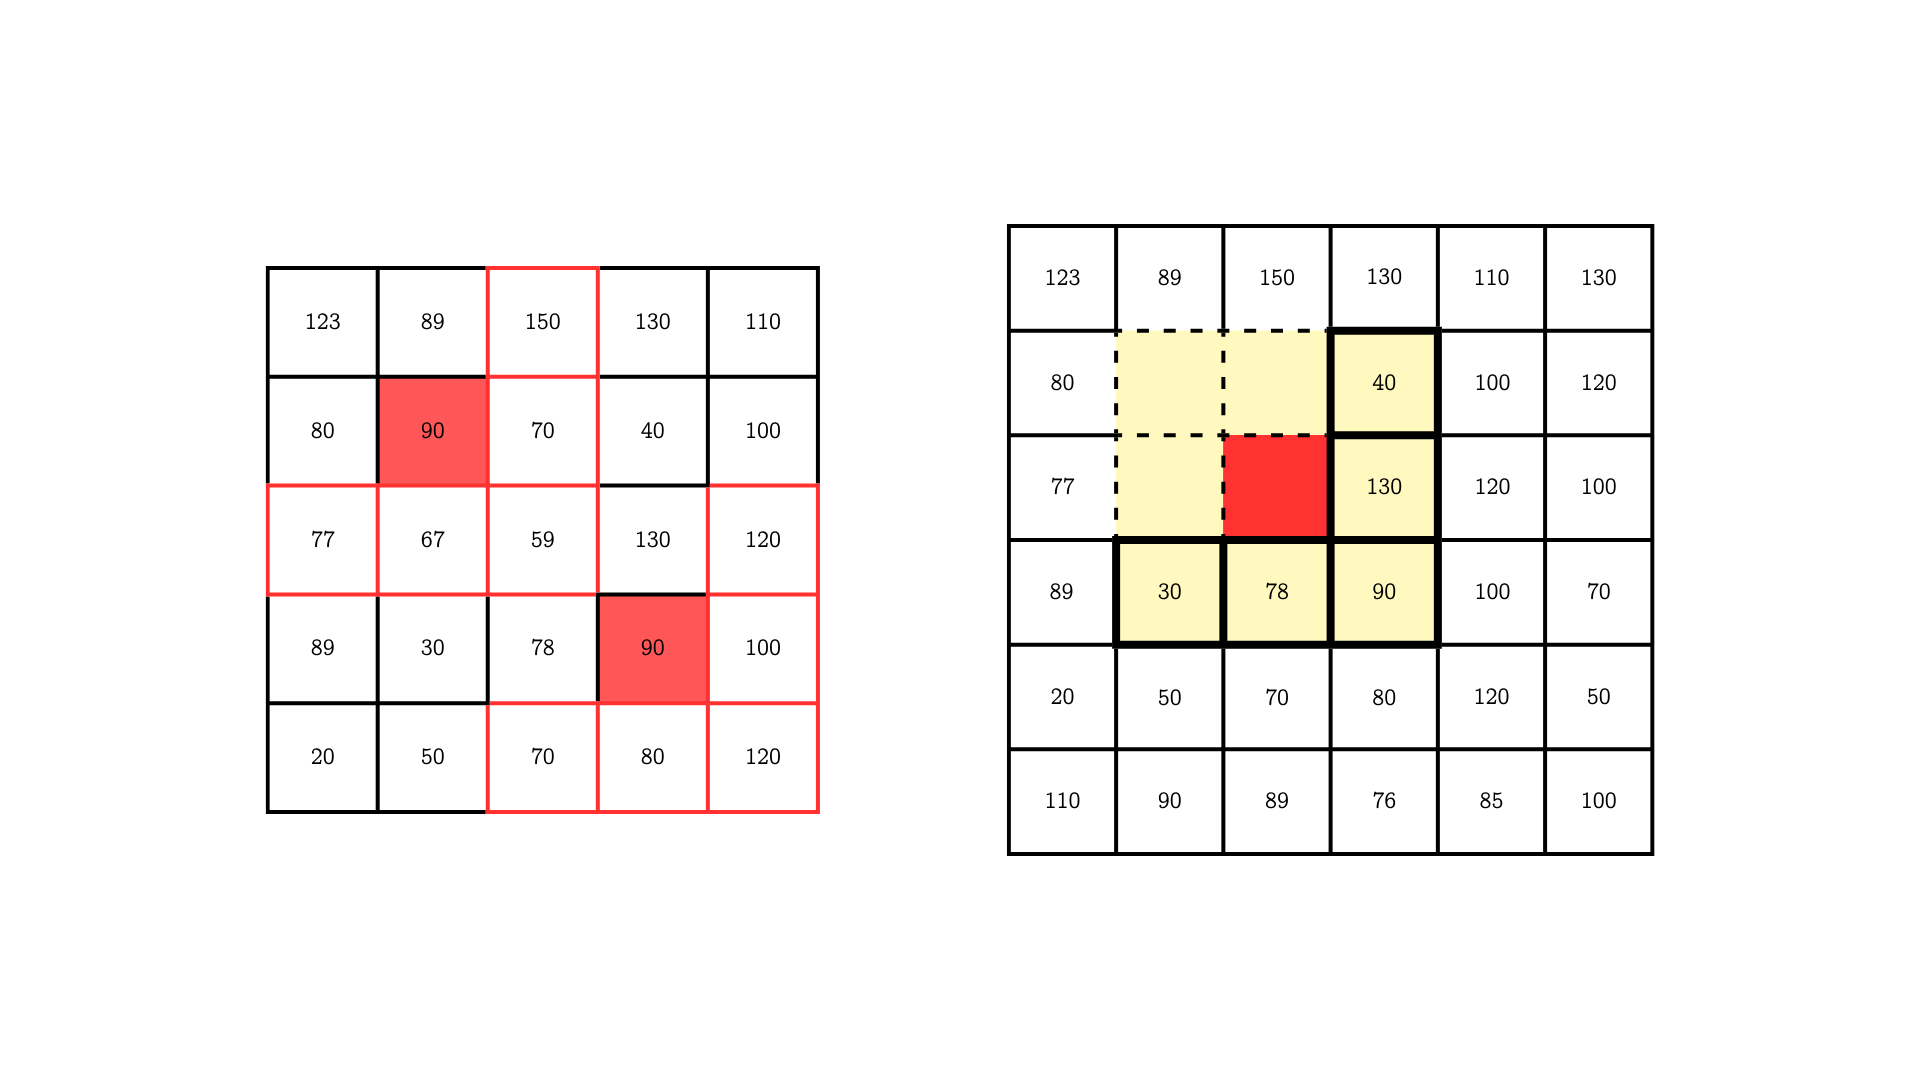
\includegraphics[width=1\textwidth]{4.png} % Replace with your image file name
        \captionsetup{labelformat=empty}
    \end{figure}
\end{frame}

\begin{frame}{Results}
    \begin{figure}[h]
    \centering
    \begin{minipage}{0.32\textwidth}
        \centering
        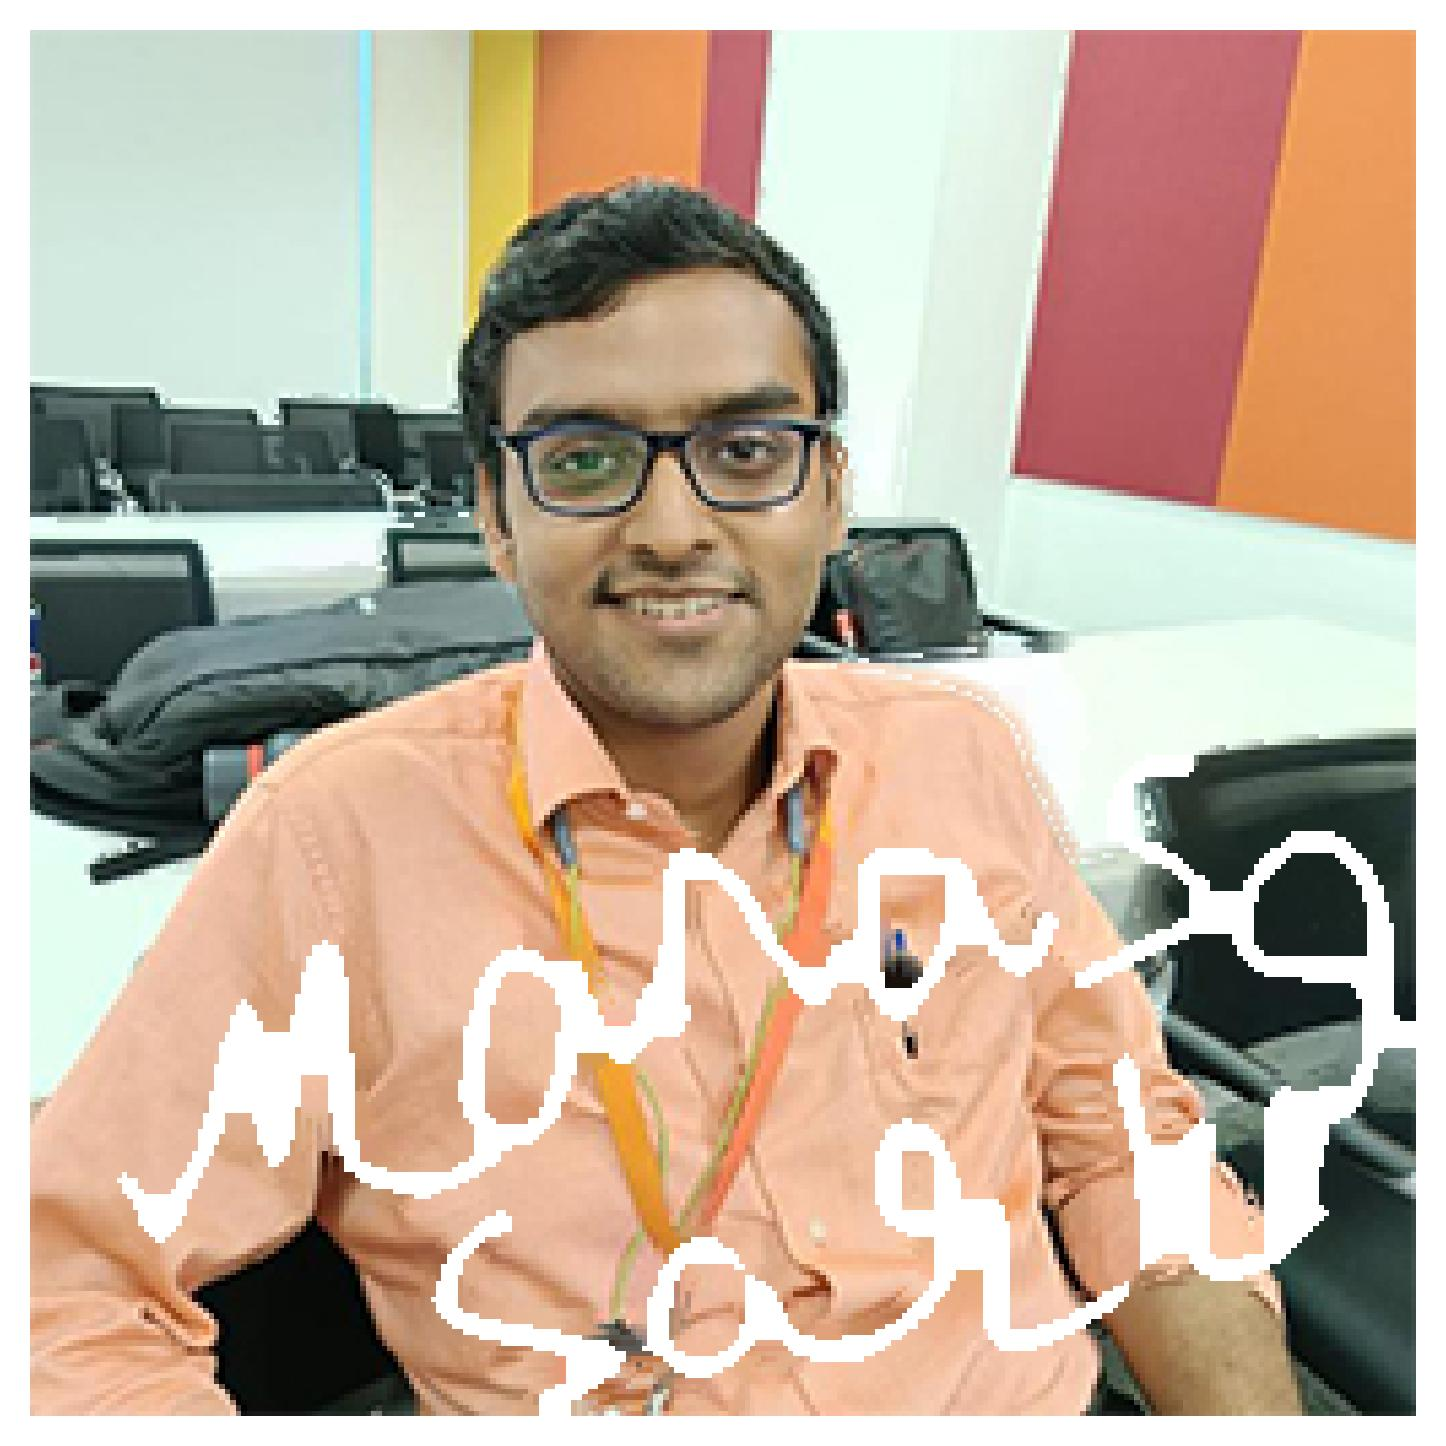
\includegraphics[width=\linewidth]{Image_inpainted_ts.jpg} % Replace with your image file
        \caption{Inpainted Image with 5*5 window}
    \end{minipage}
    \hfill
    \begin{minipage}{0.32\textwidth}
        \centering
        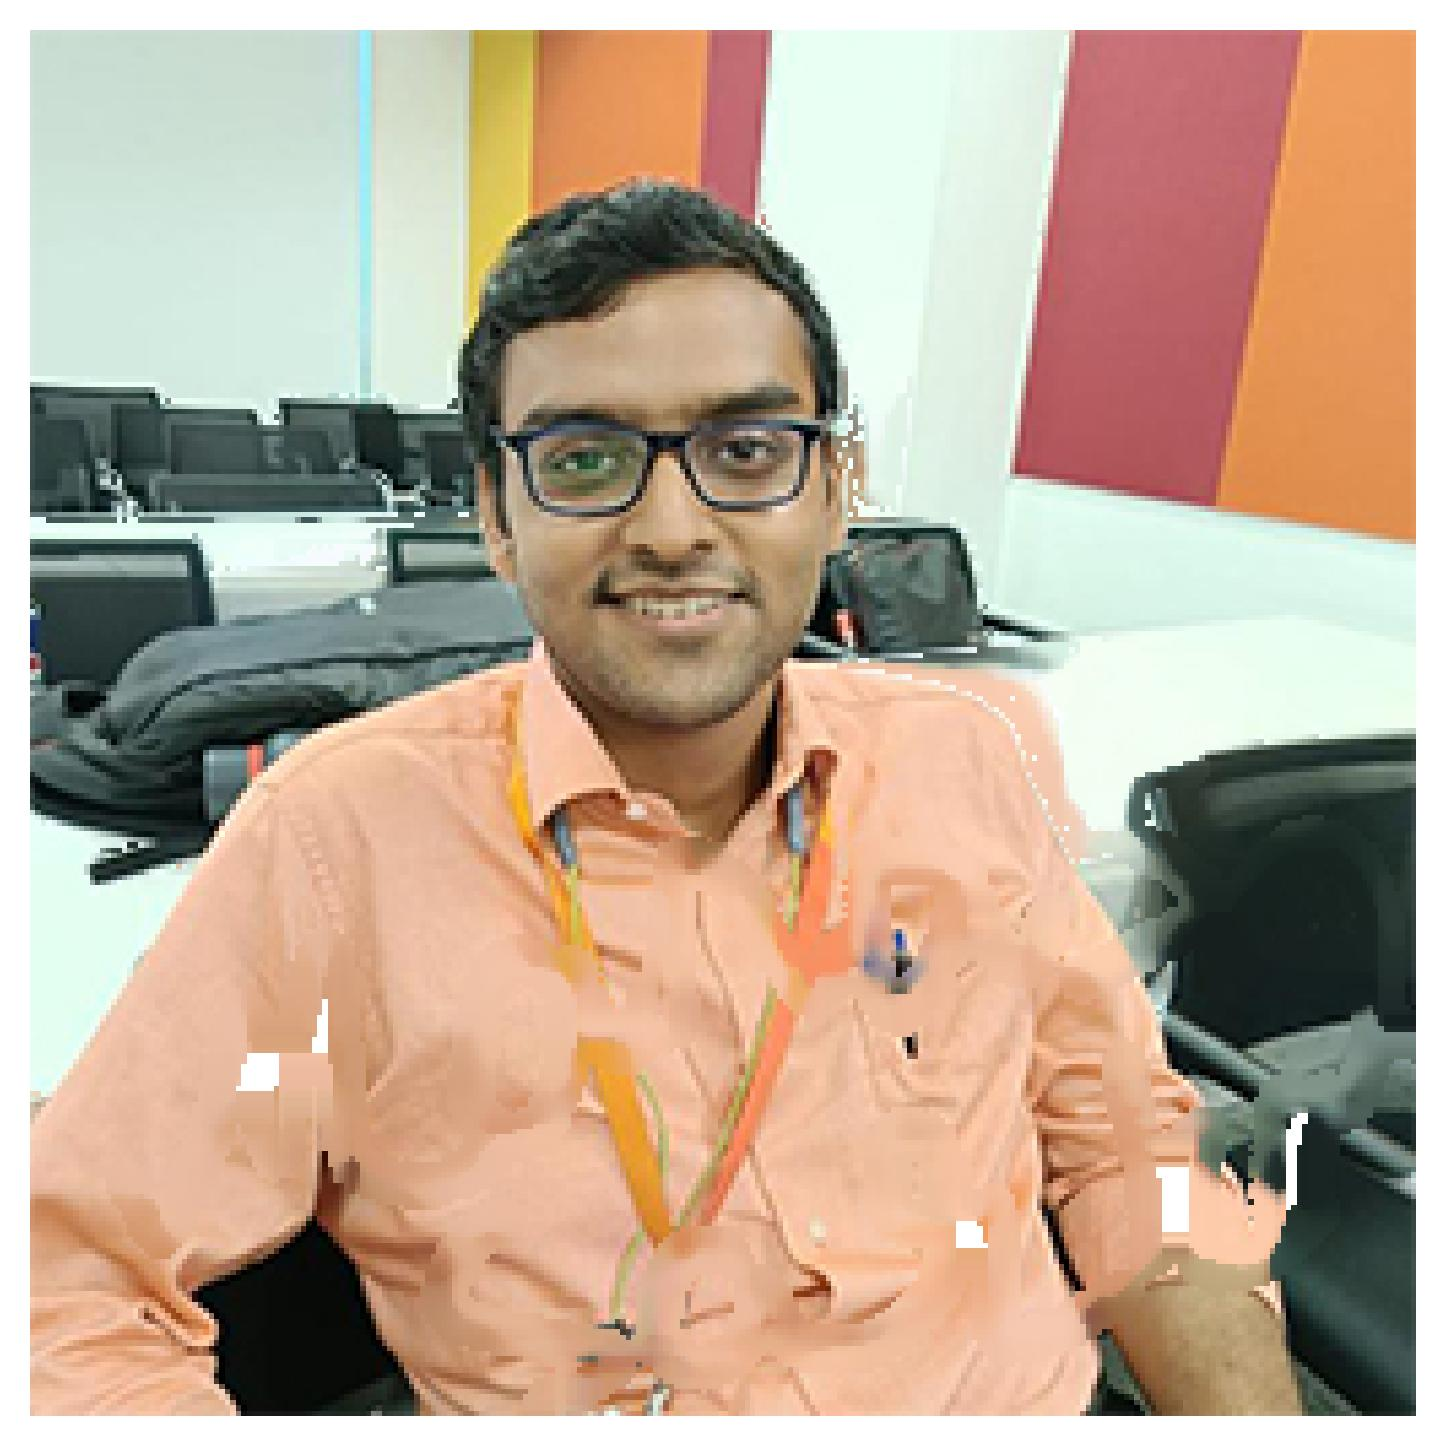
\includegraphics[width=\linewidth]{Image_inpainted_ts_13.jpg} % Replace with your image file
        \caption{Inpainted Image with 13*13 window}
    \end{minipage}
    \hfill
    \begin{minipage}{0.32\textwidth}
        \centering
        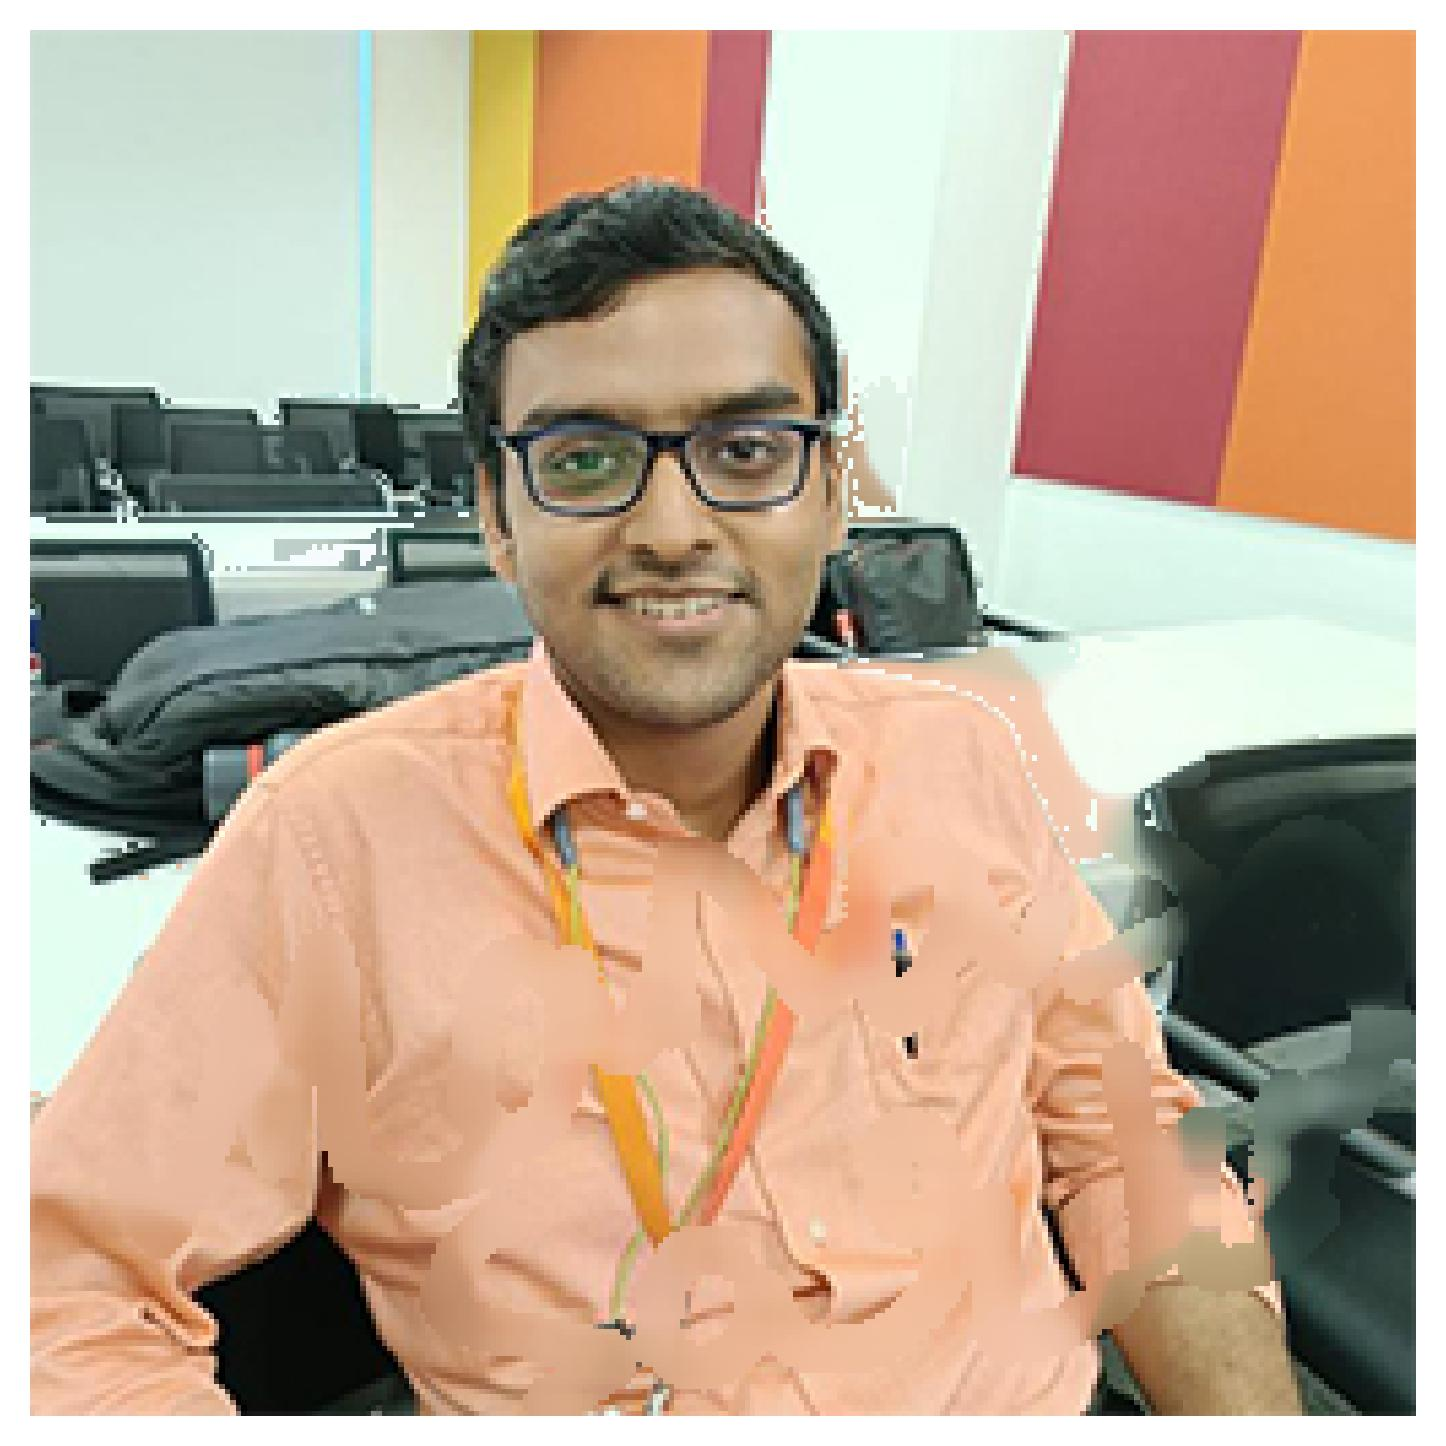
\includegraphics[width=\linewidth]{Image_inpainted_ts_25.jpg} % Replace with your image file
        \caption{Inpainted Image with 25*25 window}
    \end{minipage}
\end{figure}
    
\end{frame}


\begin{frame}{Results}
    \begin{figure}[h]
    \centering
    \begin{minipage}{0.45\textwidth}
        \centering
        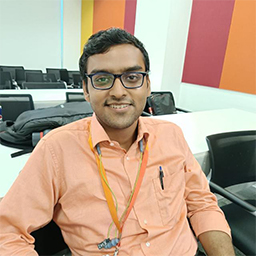
\includegraphics[width=\linewidth]{Image.jpg} % Replace with your image file name
        \caption{Original Image}
    \end{minipage}
    \hfill
    \begin{minipage}{0.45\textwidth}
        \centering
        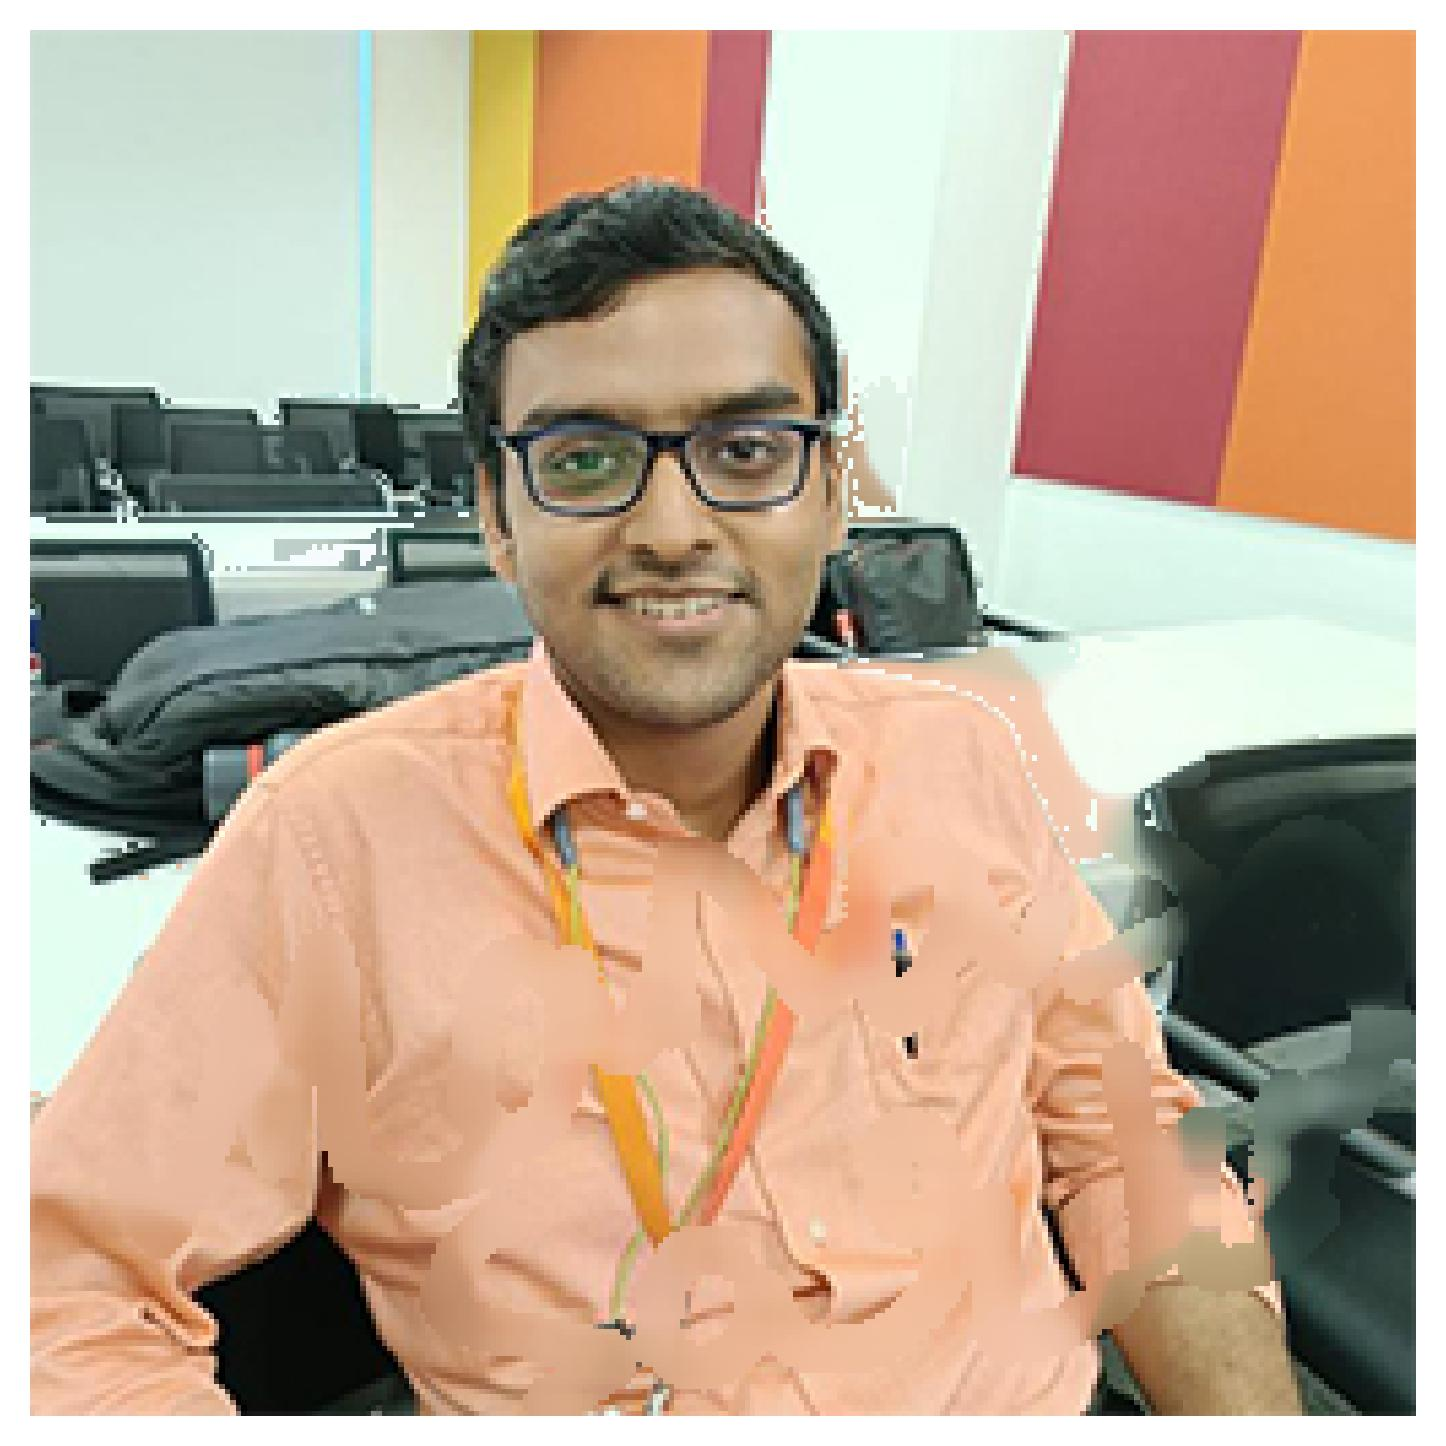
\includegraphics[width=\linewidth]{Image_inpainted_ts_25.jpg} % Replace with your image file name
        \caption{Inpainted Image with 25*25 window}
    \end{minipage}
\end{figure}
    
\end{frame}


\begin{frame}{Discussions}
    \textbf{Some Key Points}
    \begin{itemize}
        \item Very Simple
        \item Surprisingly good results 
        \item But very slow
        \item Limited in terms of mask size, accuracy and sometimes efficiency
    \end{itemize}
    
\end{frame}

%GAN based Algorithm
\section{General Adversarial Networks}

\begin{frame}{}
    \centering
    \Huge{General Adversarial Networks}
\end{frame}

\begin{frame}{Introduction}
    GAN consists of two neural networks. One is called the generator, and the other is the discriminator. 
    
    \begin{figure}[h]
        \centering
        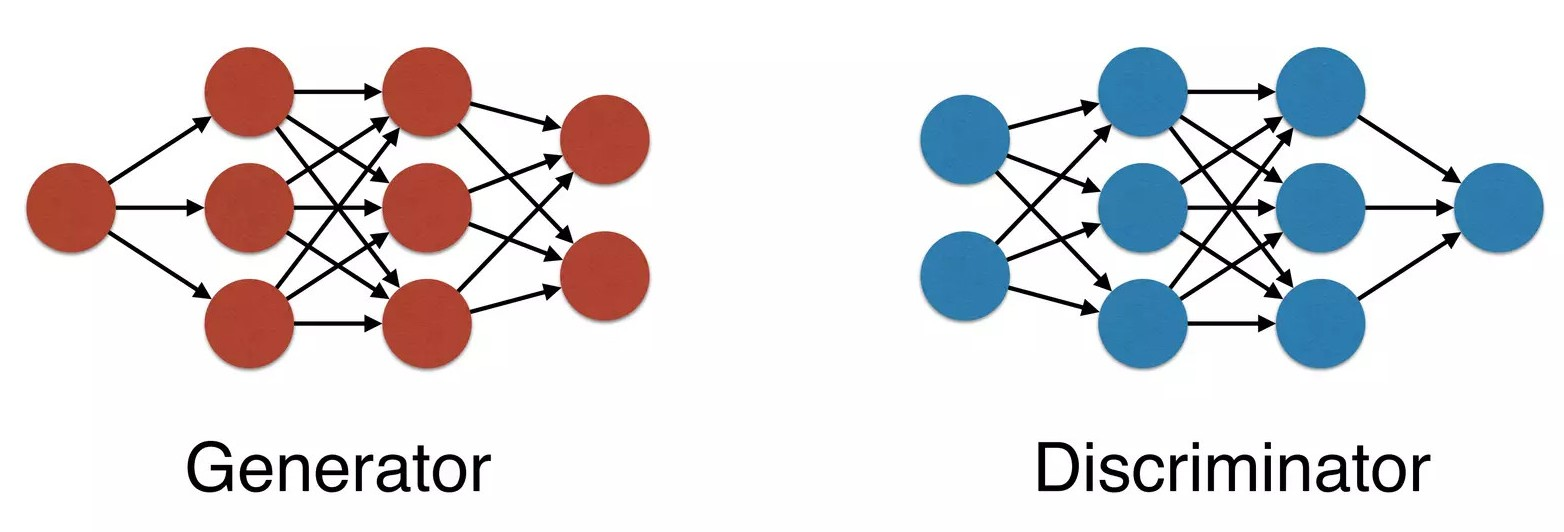
\includegraphics[width=0.8\textwidth]{slide_05.jpg} % Replace with your image file name
        \captionsetup{labelformat=empty}
    \end{figure}
    
\end{frame}

\begin{frame}{Introduction} 
    \begin{figure}[h]
        \centering
        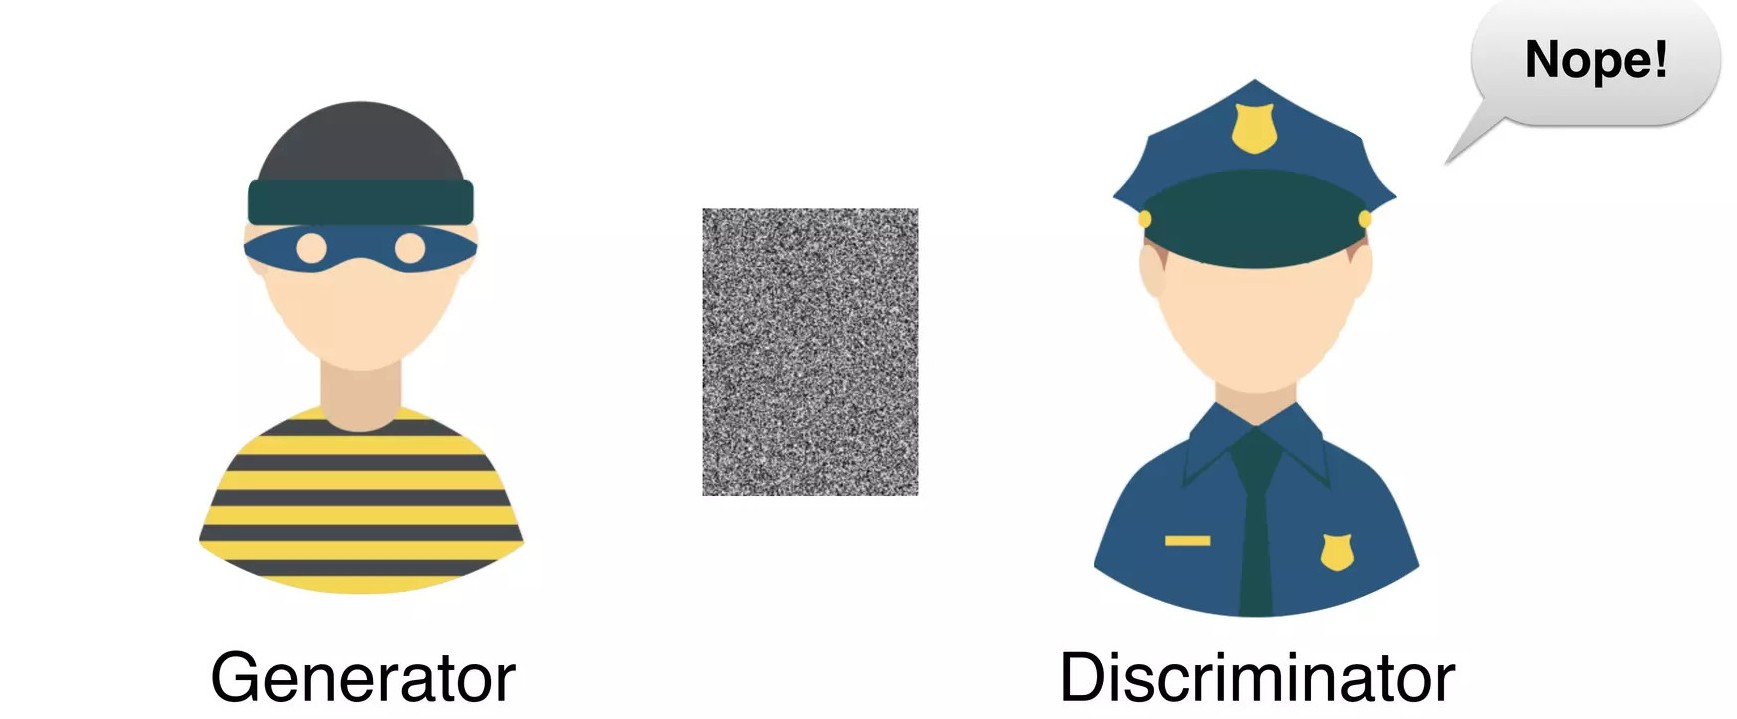
\includegraphics[width=1.0\textwidth]{slide_06.jpg} % Replace with your image file name
        \captionsetup{labelformat=empty}
    \end{figure}
    
\end{frame}

\begin{frame}{Introduction} 
    \begin{figure}[h]
        \centering
        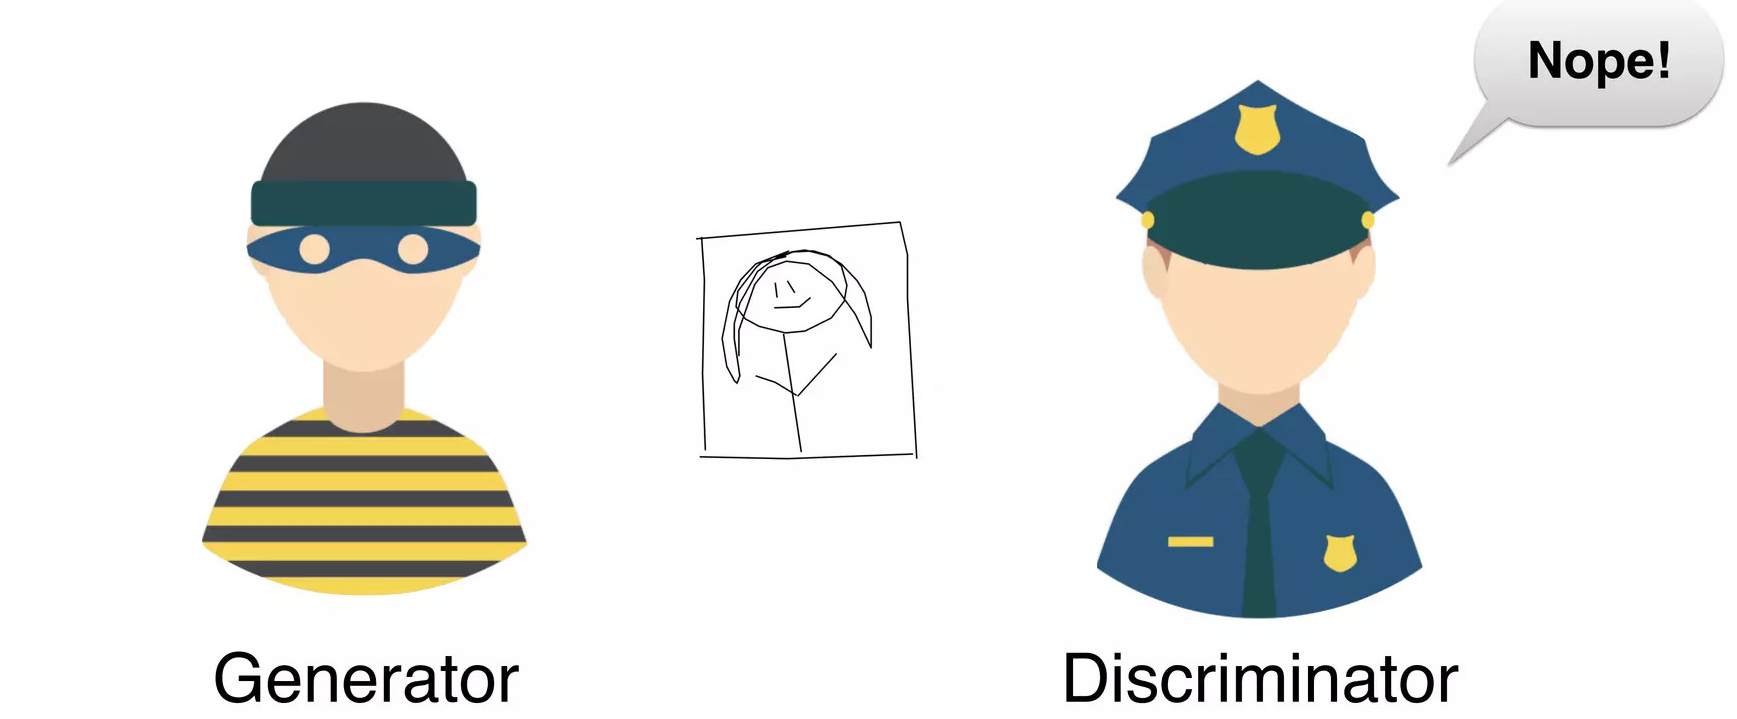
\includegraphics[width=1.0\textwidth]{slide_07.jpg} % Replace with your image file name
        \captionsetup{labelformat=empty}
    \end{figure}
    
\end{frame}

\begin{frame}{Introduction} 
    \begin{figure}[h]
        \centering
        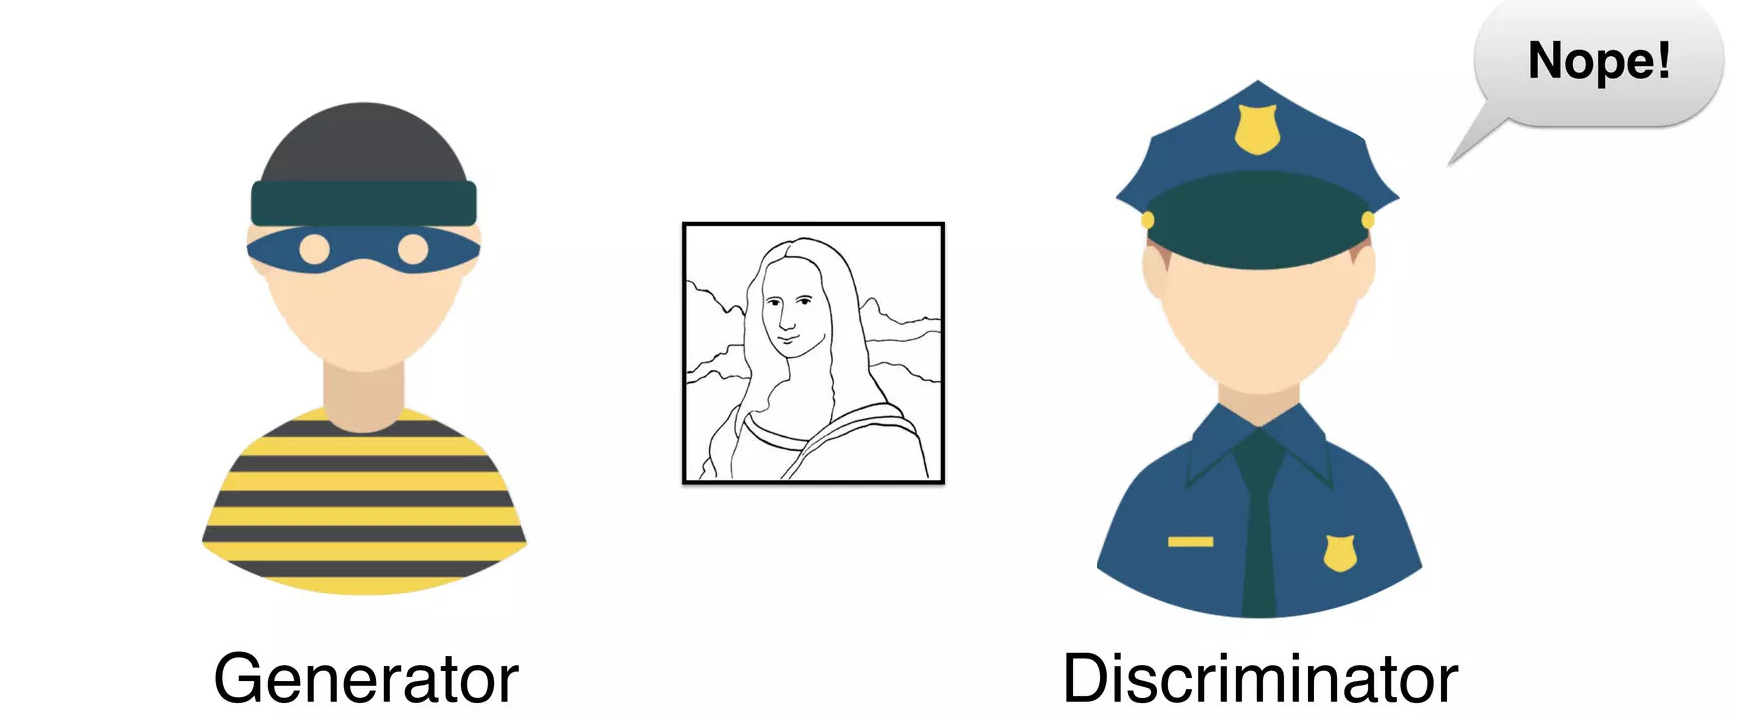
\includegraphics[width=1.0\textwidth]{slide_08.jpg} % Replace with your image file name
        \captionsetup{labelformat=empty}
    \end{figure}
    
\end{frame}

\begin{frame}{Introduction} 
    \begin{figure}[h]
        \centering
        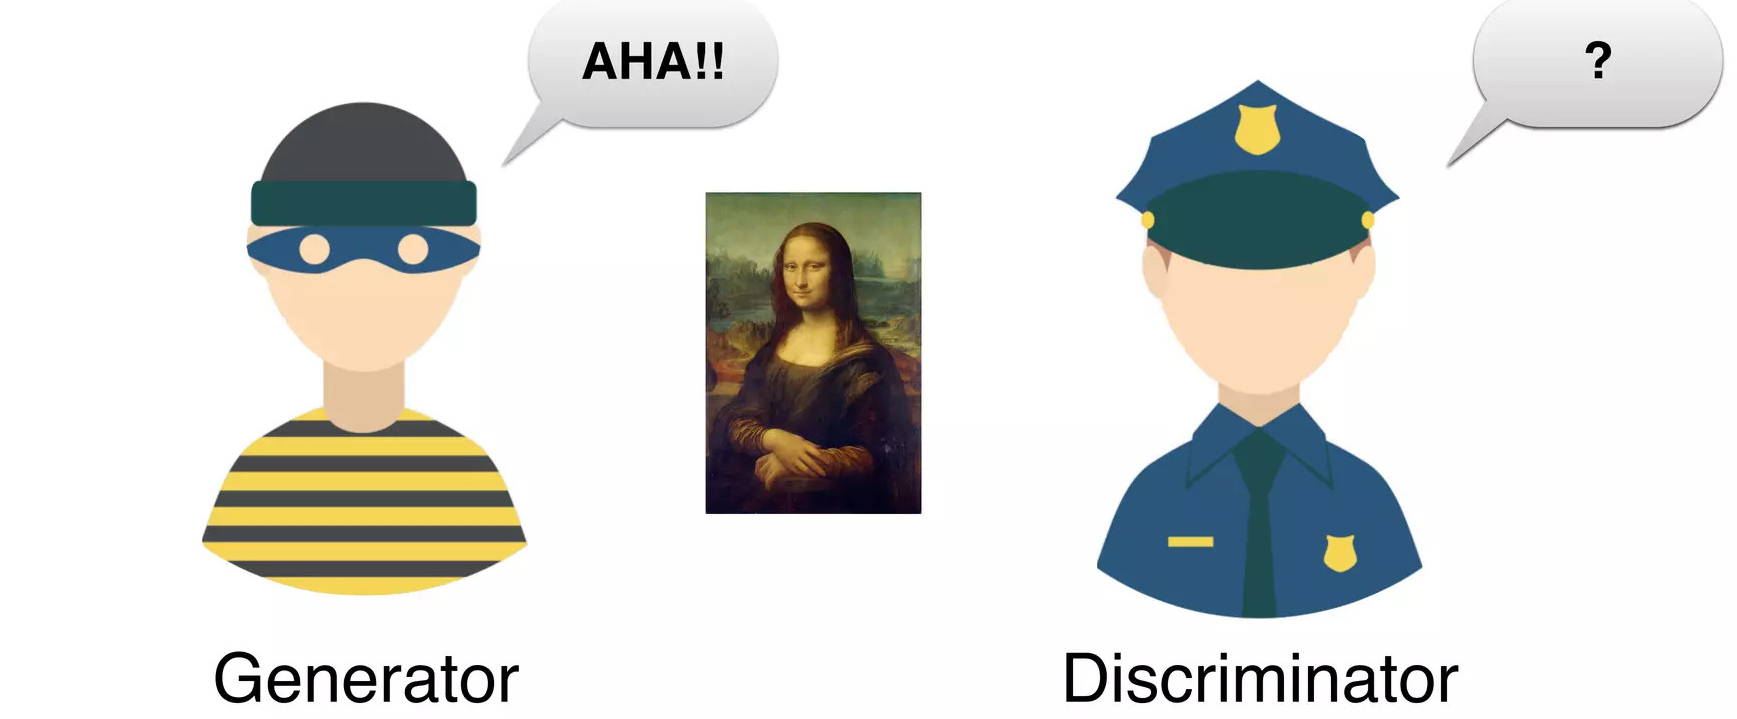
\includegraphics[width=1.0\textwidth]{slide_10.jpg} % Replace with your image file name
        \captionsetup{labelformat=empty}
    \end{figure}
\end{frame}

\begin{frame}{GAN Block Architecture} 
    \begin{figure}[h]
        \centering
        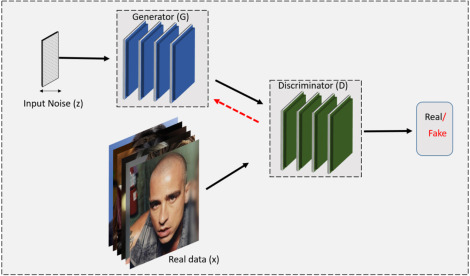
\includegraphics[width=0.7\textwidth]{Basic GAN blueprint.jpg} % Replace with your image file name
        \caption{ An example GAN block. The input of the generator (z) is sampled from a random noise vector and the input of the discriminator (x) is sampled from real data distribution.}
    \end{figure}
\end{frame}

\begin{frame}{Neural Networks} 
    \begin{figure}[h]
        \centering
        \makebox[\linewidth]{% ensures centering even if the image is wider than the text width
            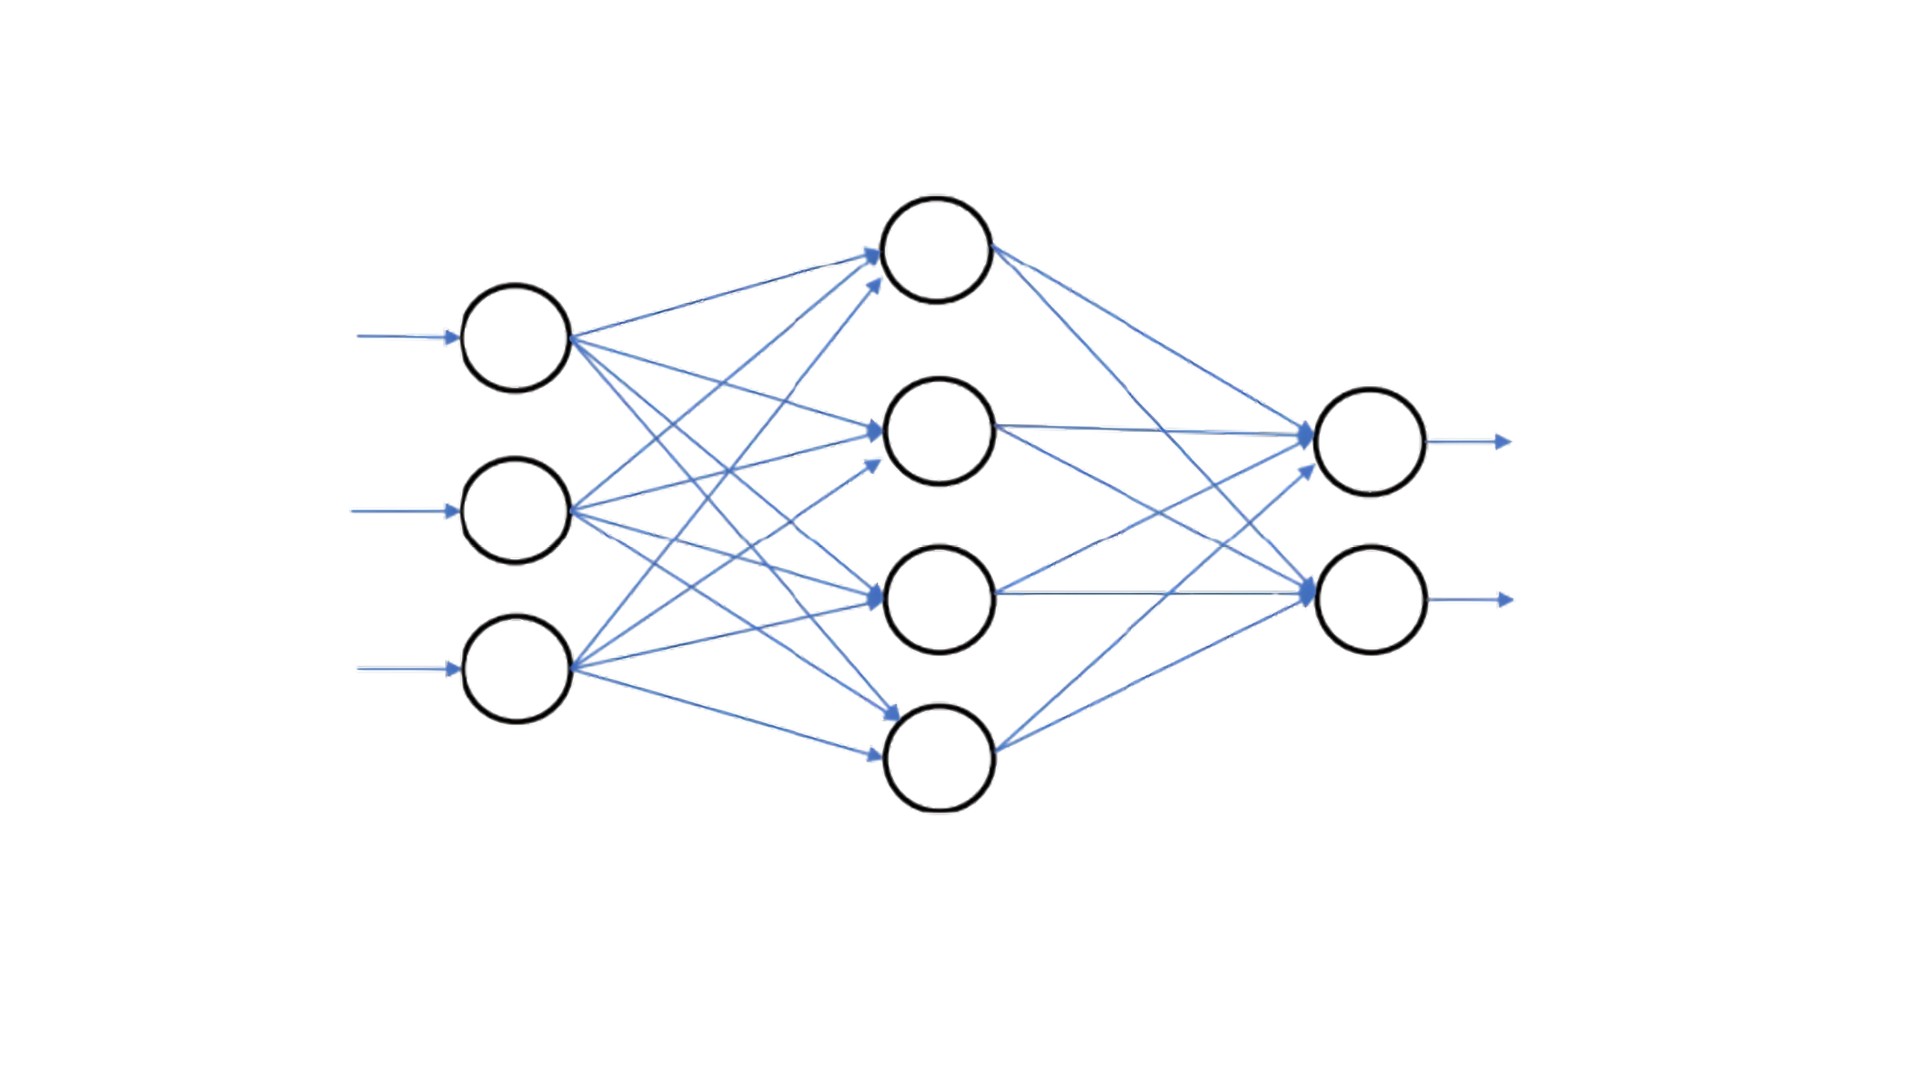
\includegraphics[width=1.3\textwidth]{Neural Network/1.png}
        }
        \captionsetup{labelformat=empty}
    \end{figure}
\end{frame}

\begin{frame}{Neural Networks} 
    \begin{figure}[h]
        \centering
        \makebox[\linewidth]{% ensures centering even if the image is wider than the text width
            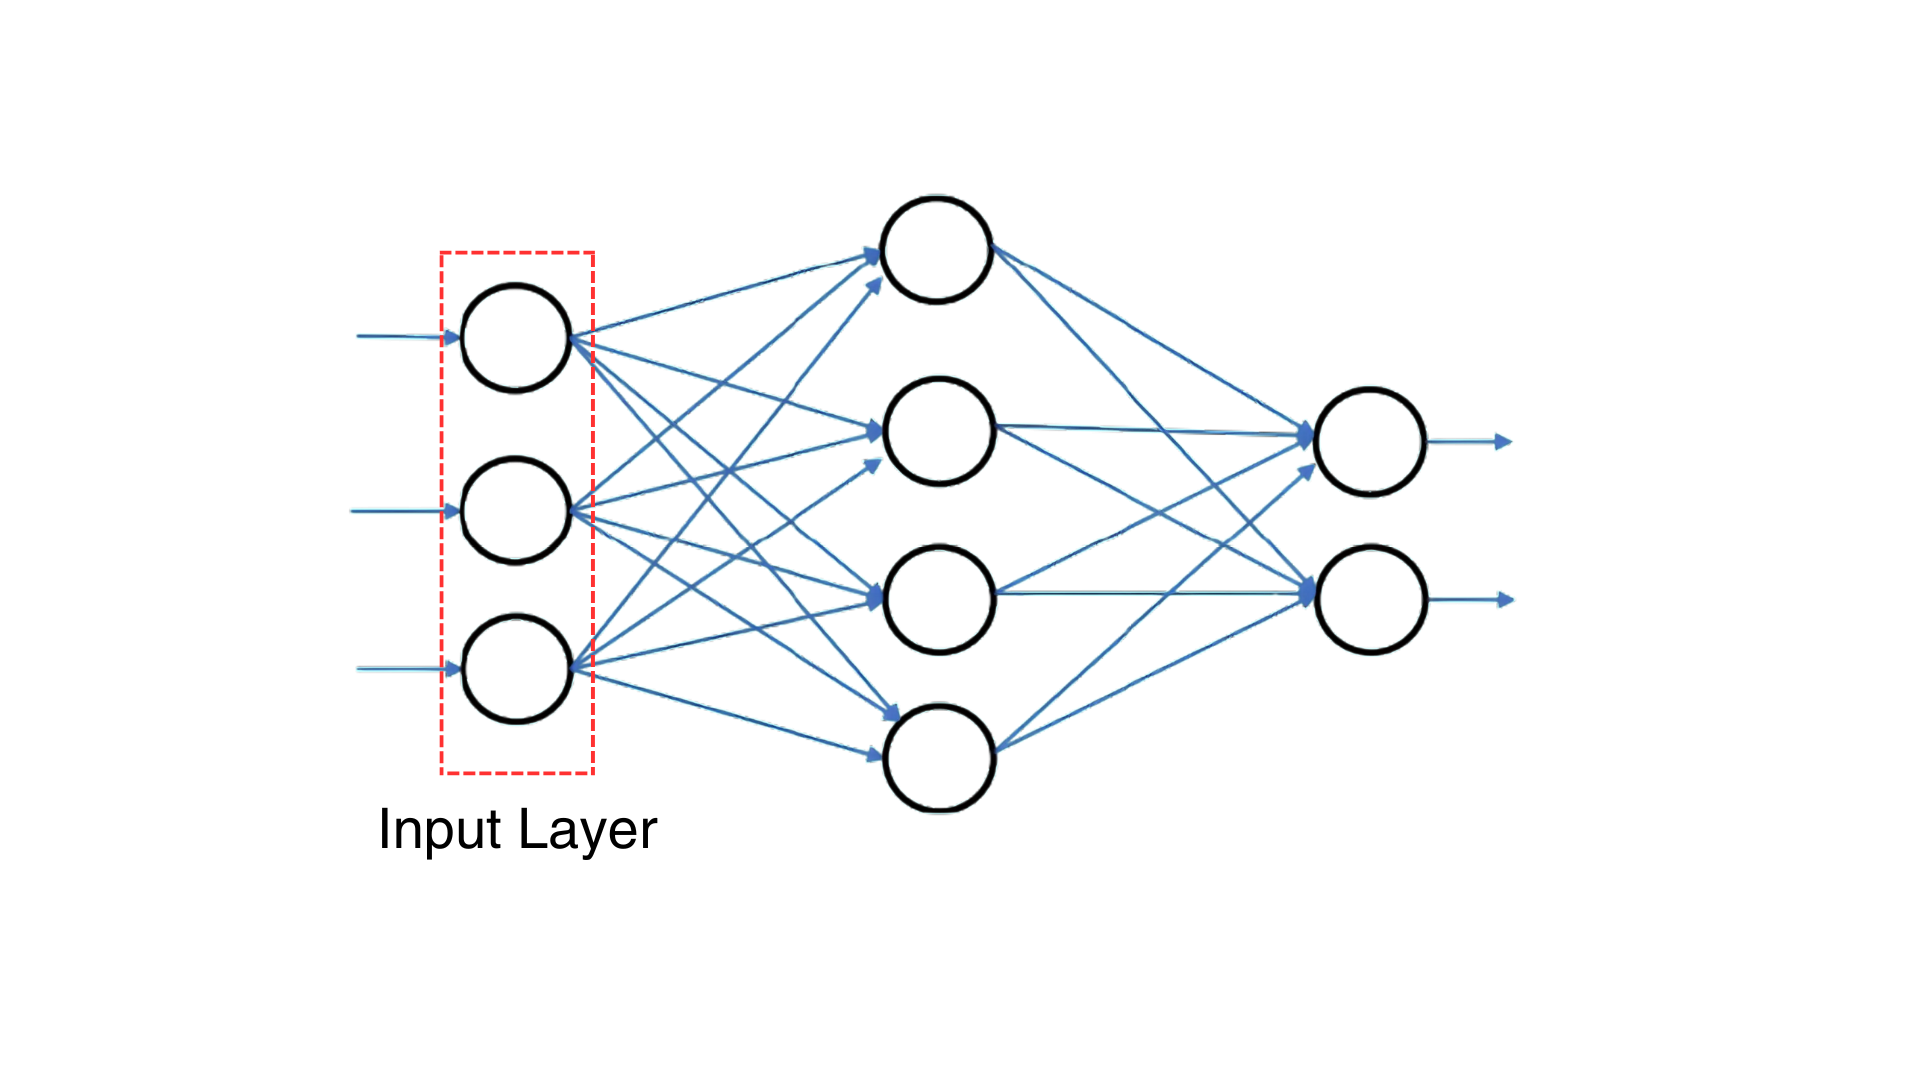
\includegraphics[width=1.3\textwidth]{Neural Network/2.png}
        }
        \captionsetup{labelformat=empty}
    \end{figure}
\end{frame}

\begin{frame}{Neural Networks} 
    \begin{figure}[h]
        \centering
        \makebox[\linewidth]{% ensures centering even if the image is wider than the text width
            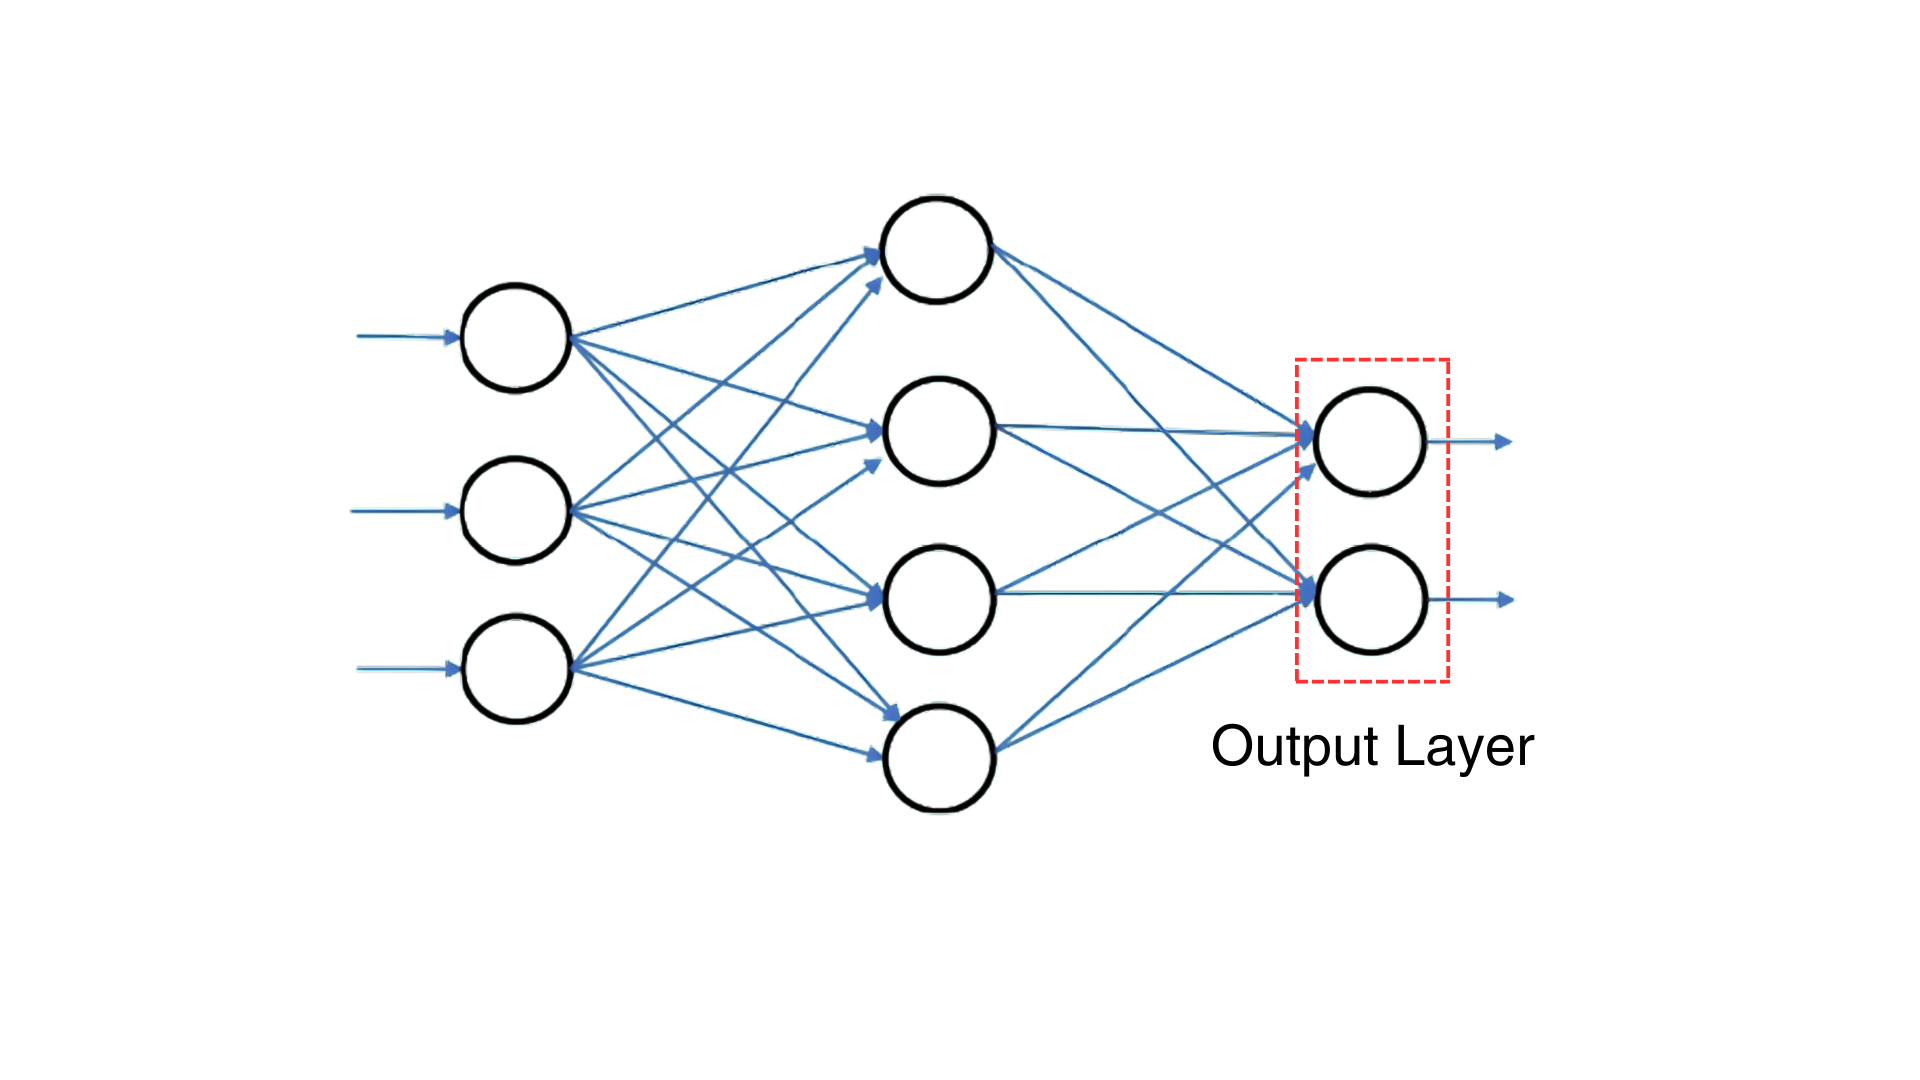
\includegraphics[width=1.3\textwidth]{Neural Network/3.png}
        }
        \captionsetup{labelformat=empty}
    \end{figure}
\end{frame}

\begin{frame}{Neural Networks} 
    \begin{figure}[h]
        \centering
        \makebox[\linewidth]{% ensures centering even if the image is wider than the text width
            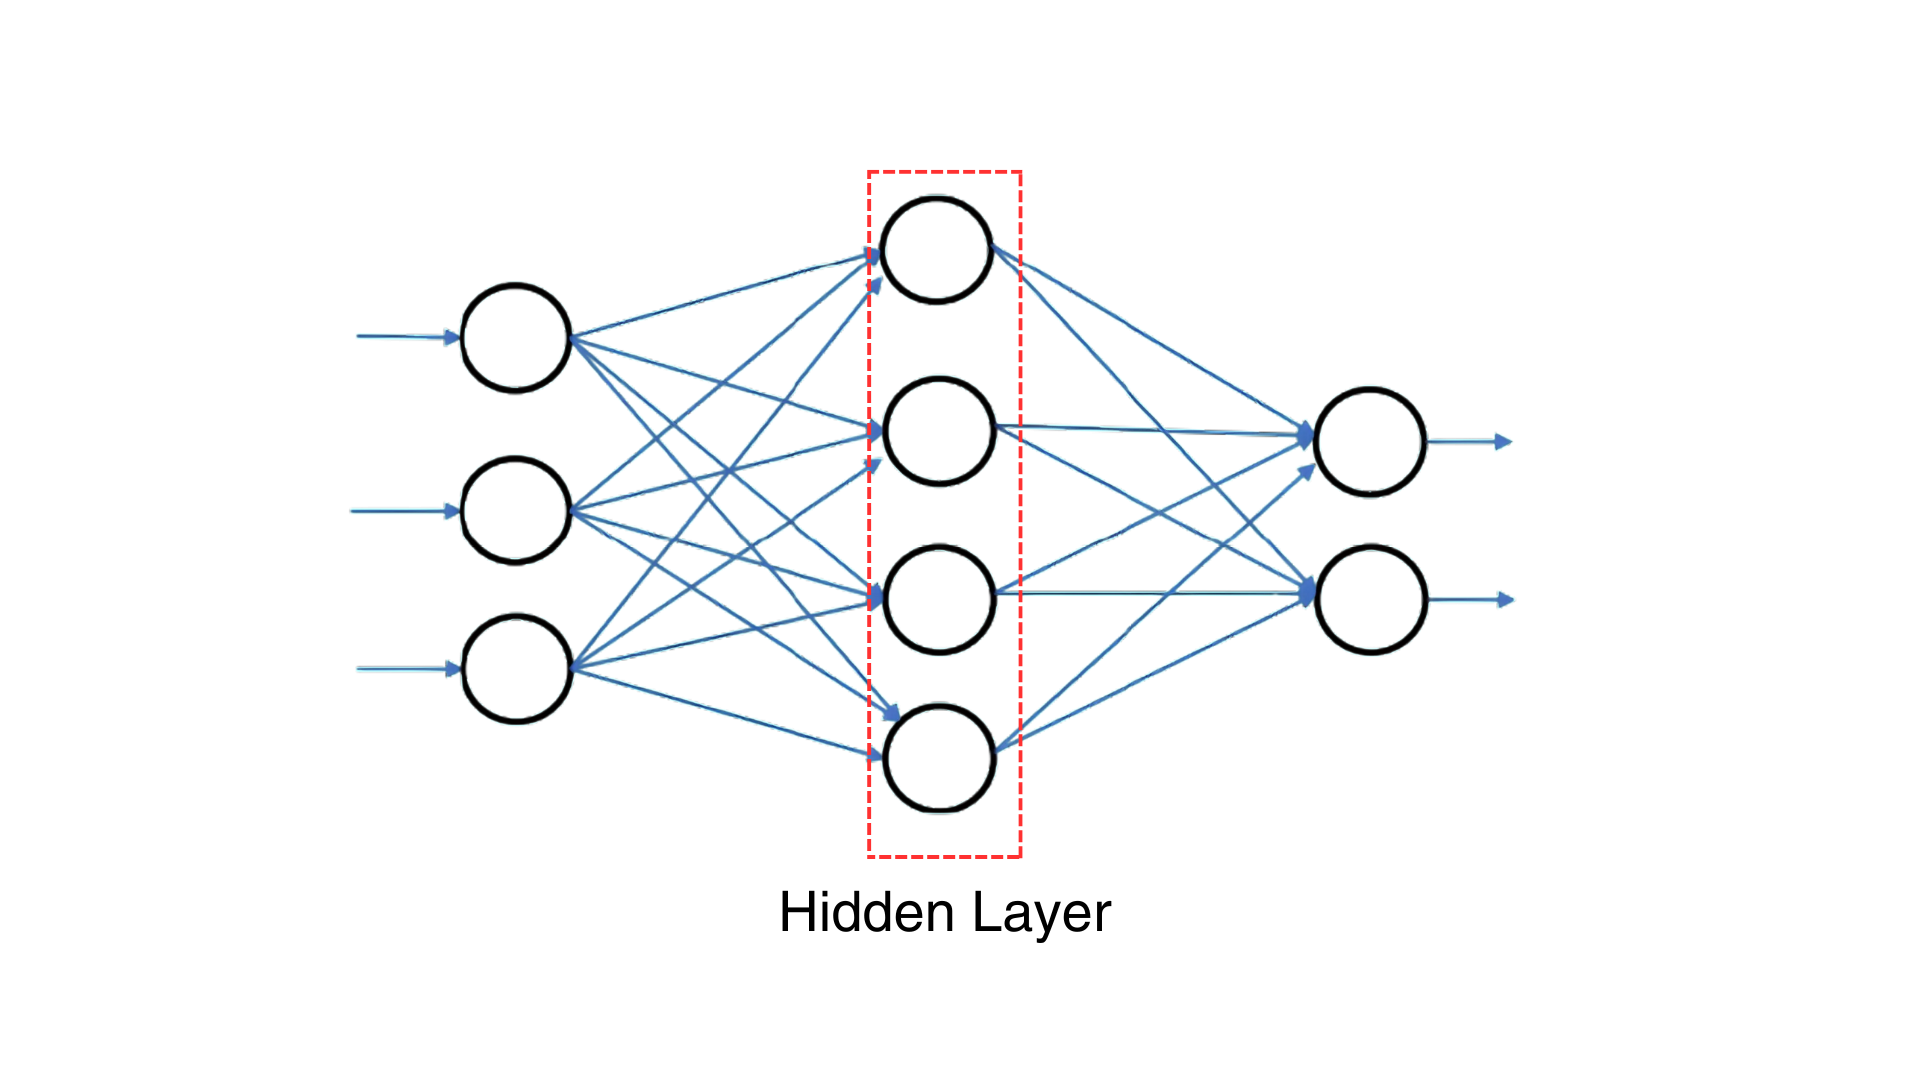
\includegraphics[width=1.3\textwidth]{Neural Network/4.png}
        }
        \captionsetup{labelformat=empty}
    \end{figure}
\end{frame}

\begin{frame}{Neural Networks} 
    \begin{figure}[h]
        \centering
        \makebox[\linewidth]{% ensures centering even if the image is wider than the text width
            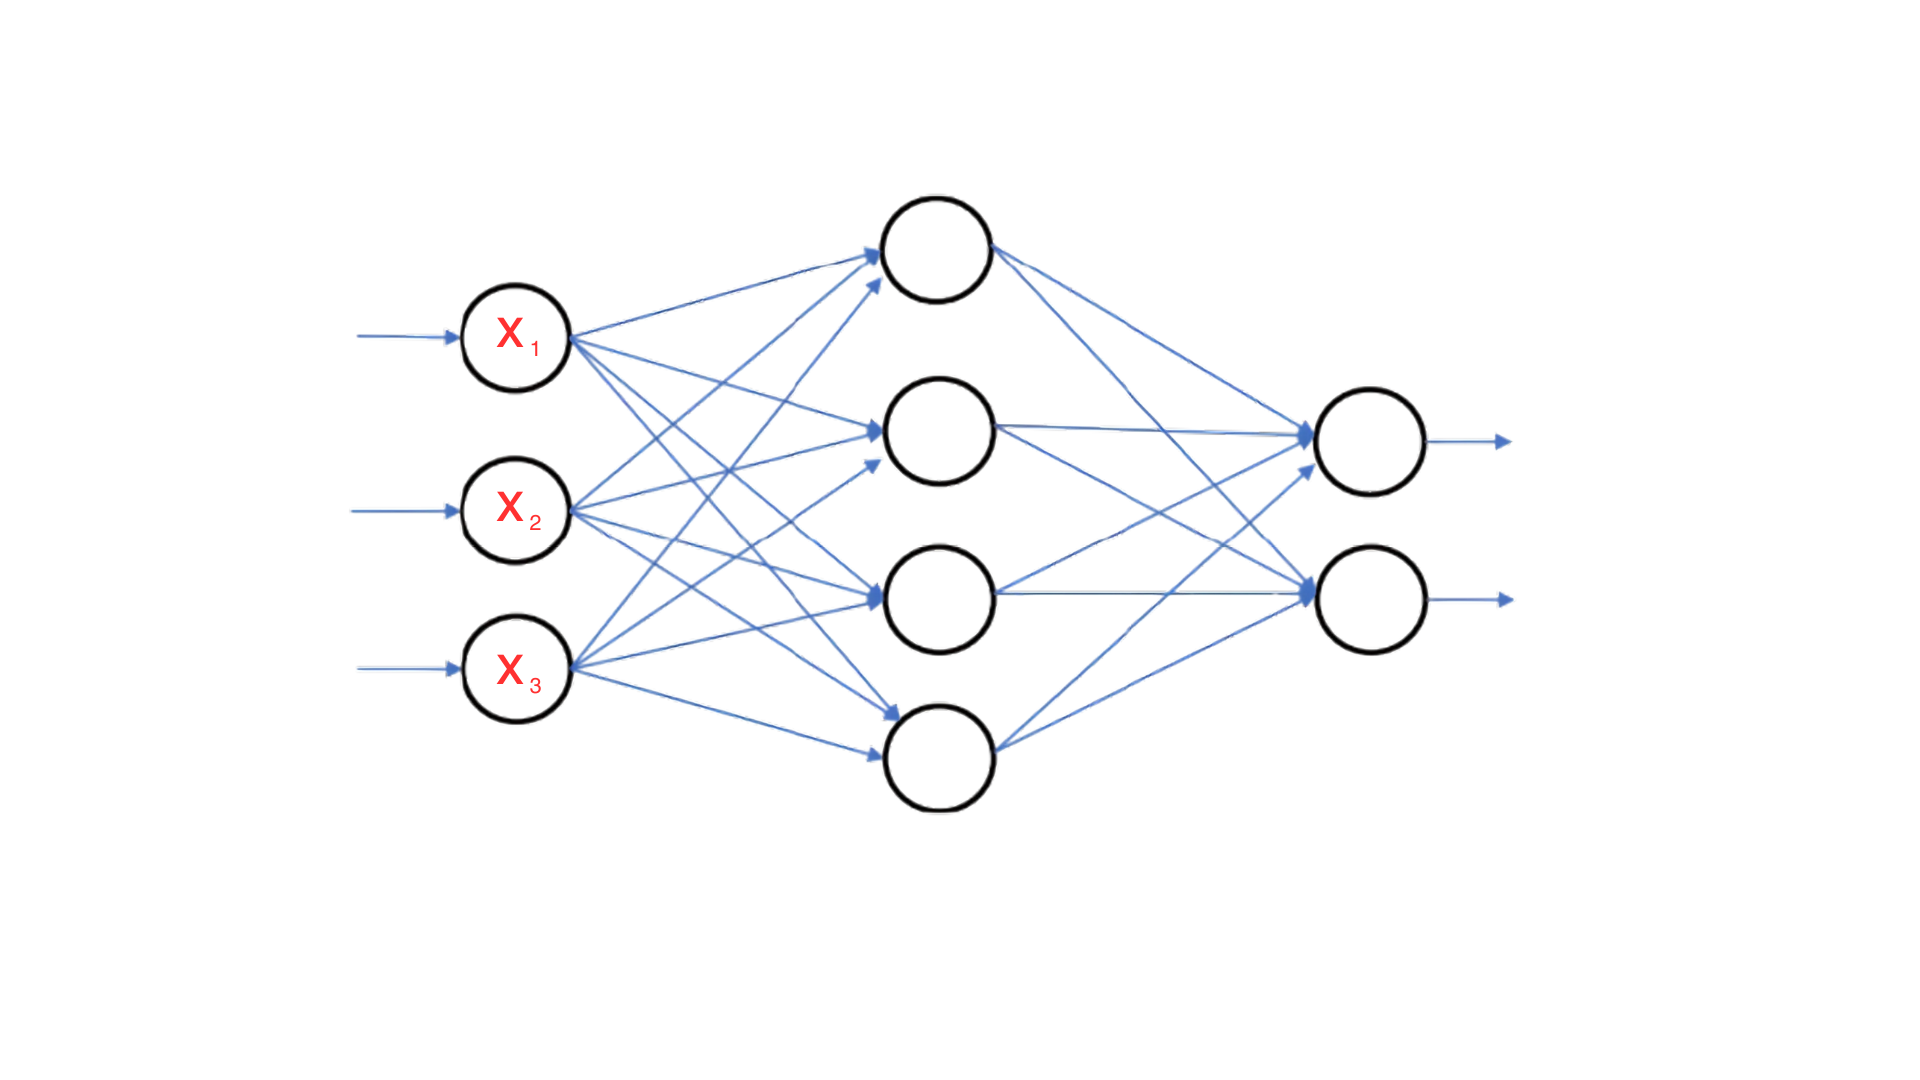
\includegraphics[width=1.3\textwidth]{Neural Network/5.png}
        }
        \captionsetup{labelformat=empty}
    \end{figure}
\end{frame}

\begin{frame}{Neural Networks} 
    \begin{figure}[h]
        \centering
        \makebox[\linewidth]{% ensures centering even if the image is wider than the text width
            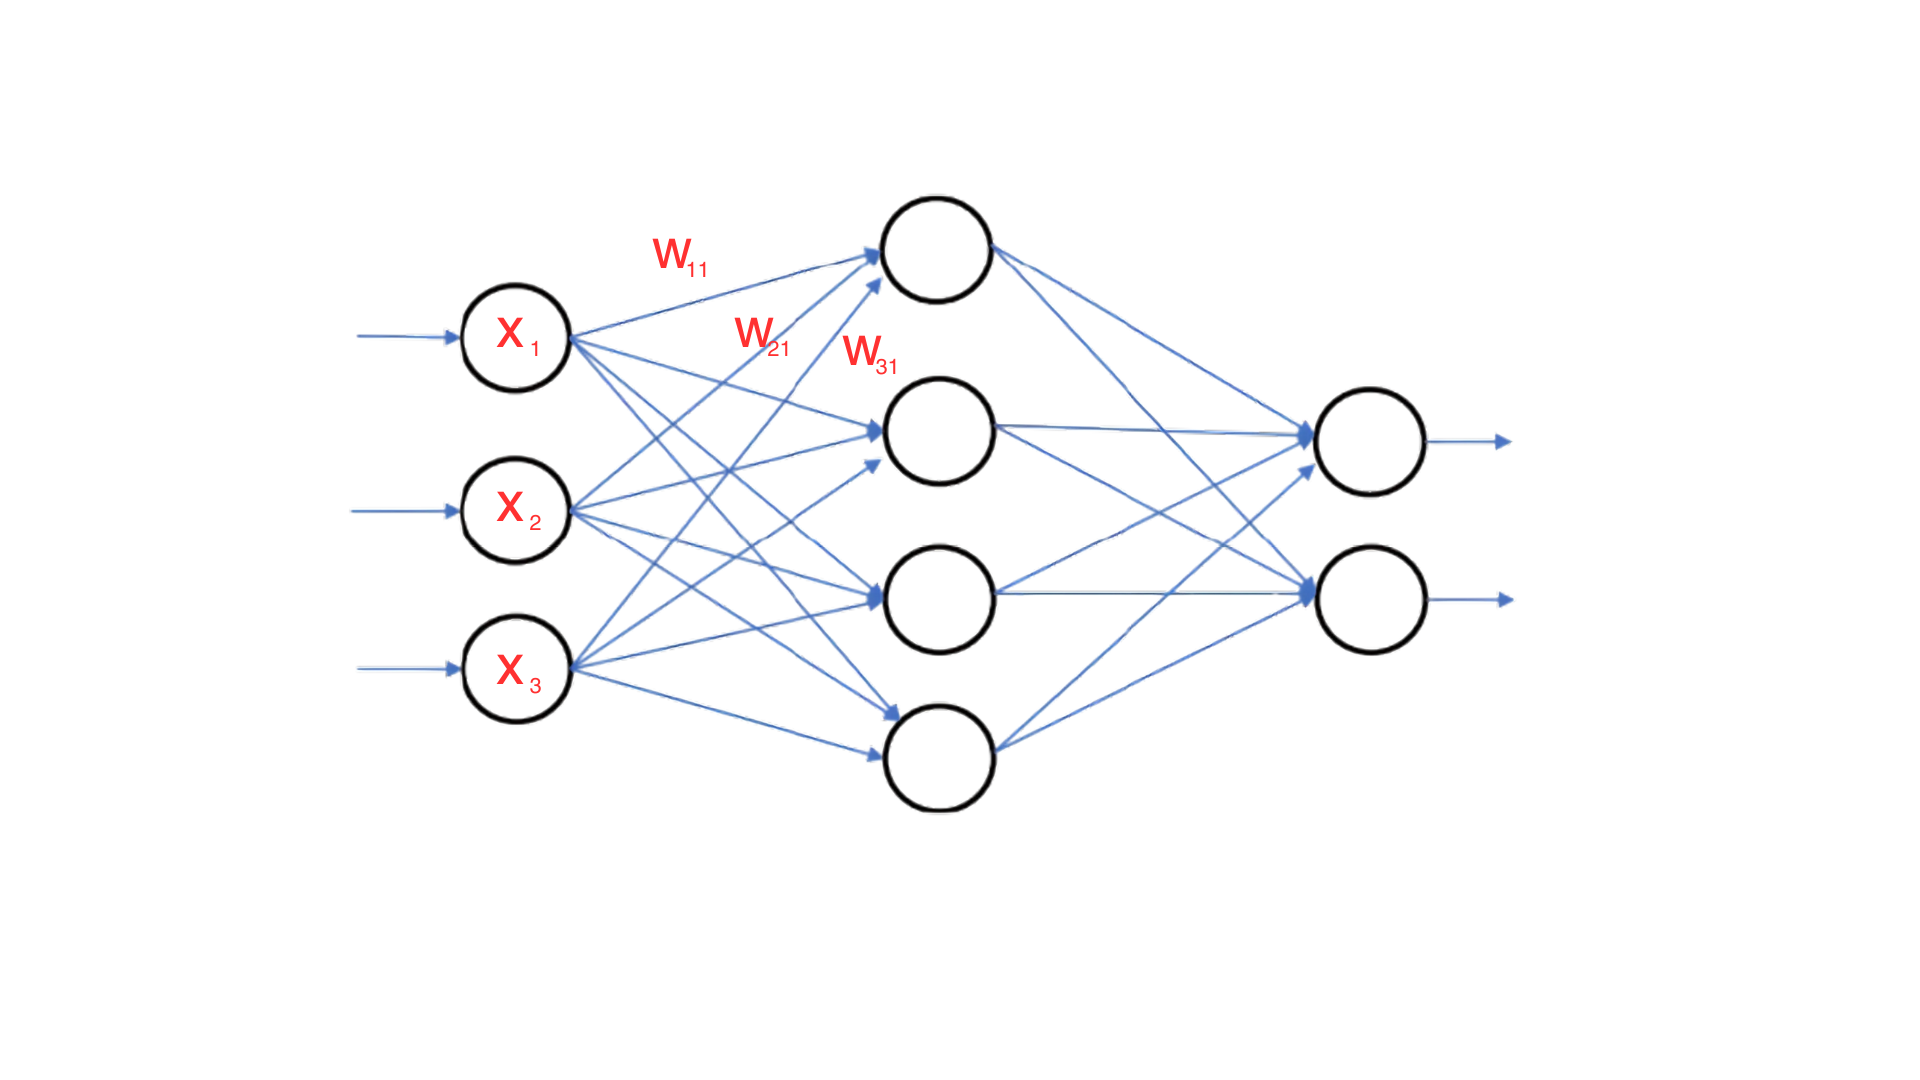
\includegraphics[width=1.3\textwidth]{Neural Network/6.png}
        }
        \captionsetup{labelformat=empty}
    \end{figure}
\end{frame}

\begin{frame}{Neural Networks} 
    \begin{figure}[h]
        \centering
        \makebox[\linewidth]{% ensures centering even if the image is wider than the text width
            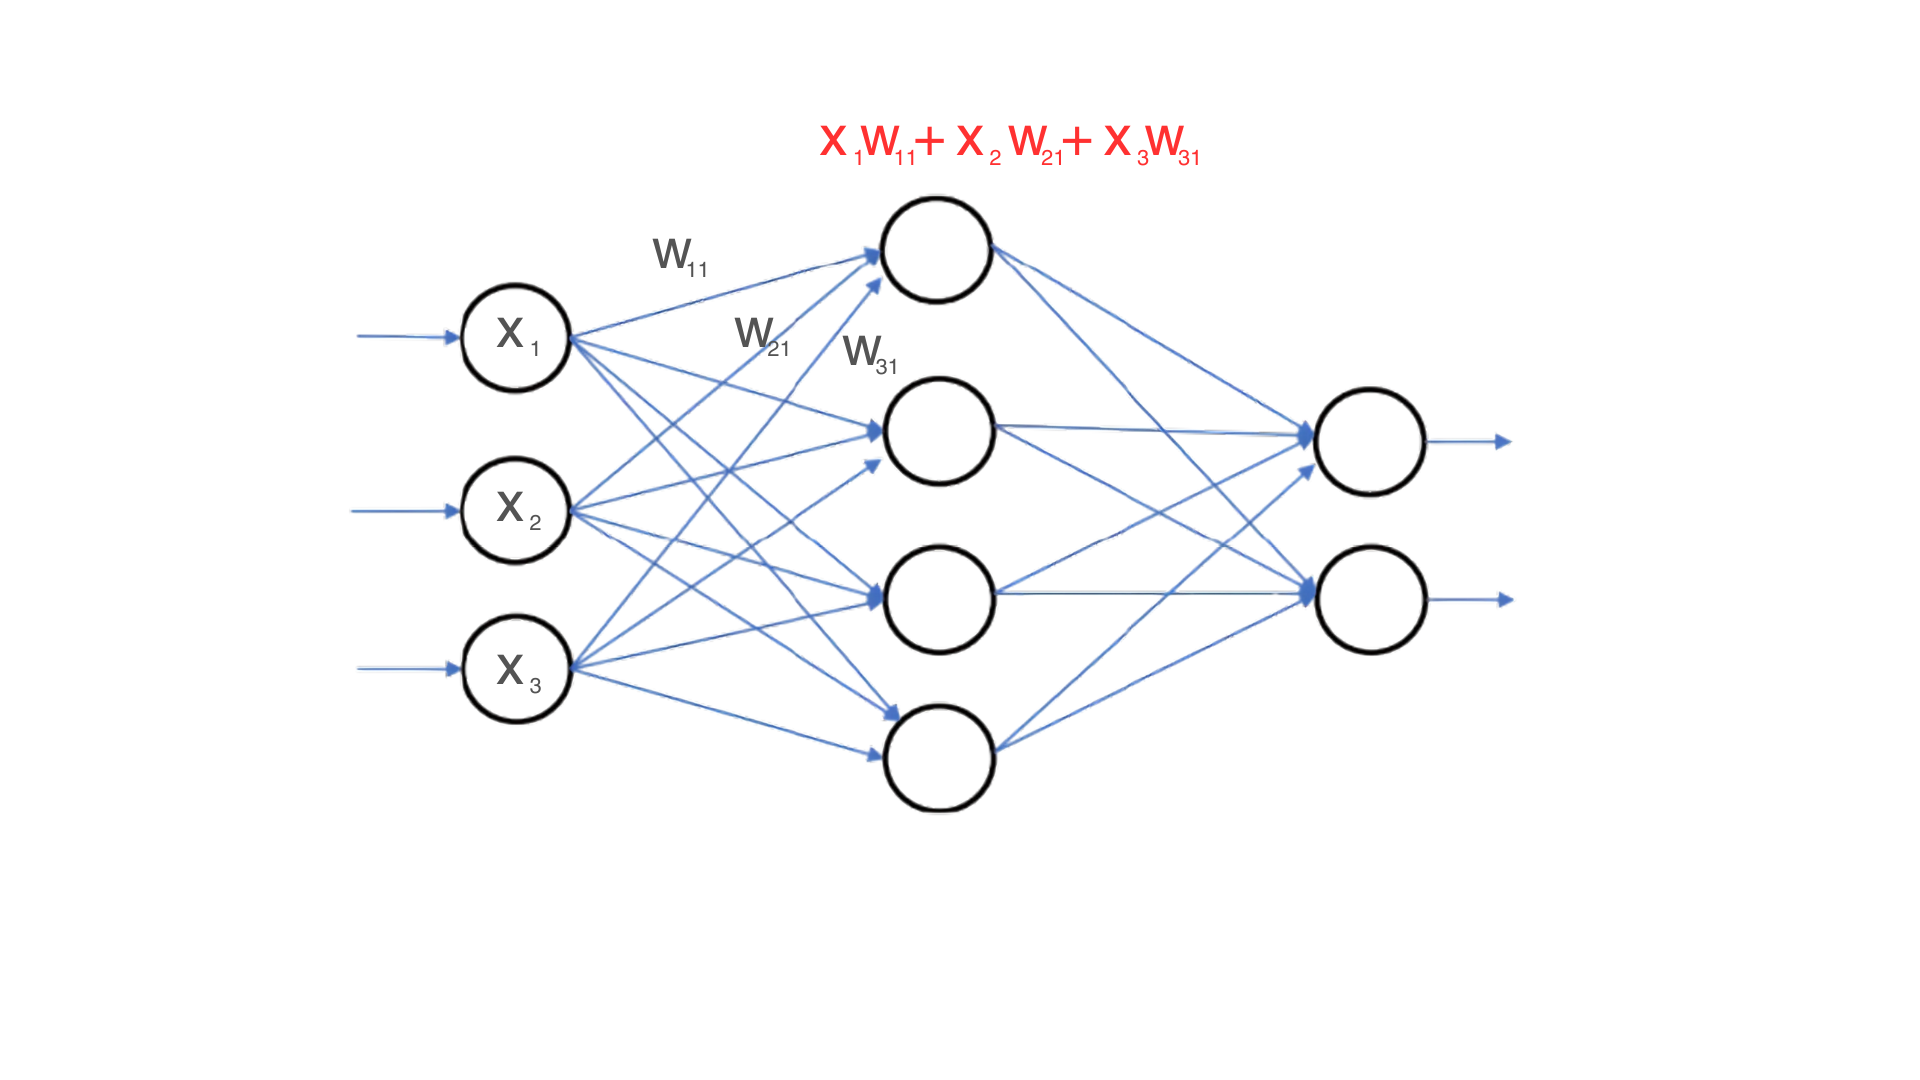
\includegraphics[width=1.3\textwidth]{Neural Network/7.png}
        }
        \captionsetup{labelformat=empty}
    \end{figure}
\end{frame}

\begin{frame}{Neural Networks} 
    \begin{figure}[h]
        \centering
        \makebox[\linewidth]{% ensures centering even if the image is wider than the text width
            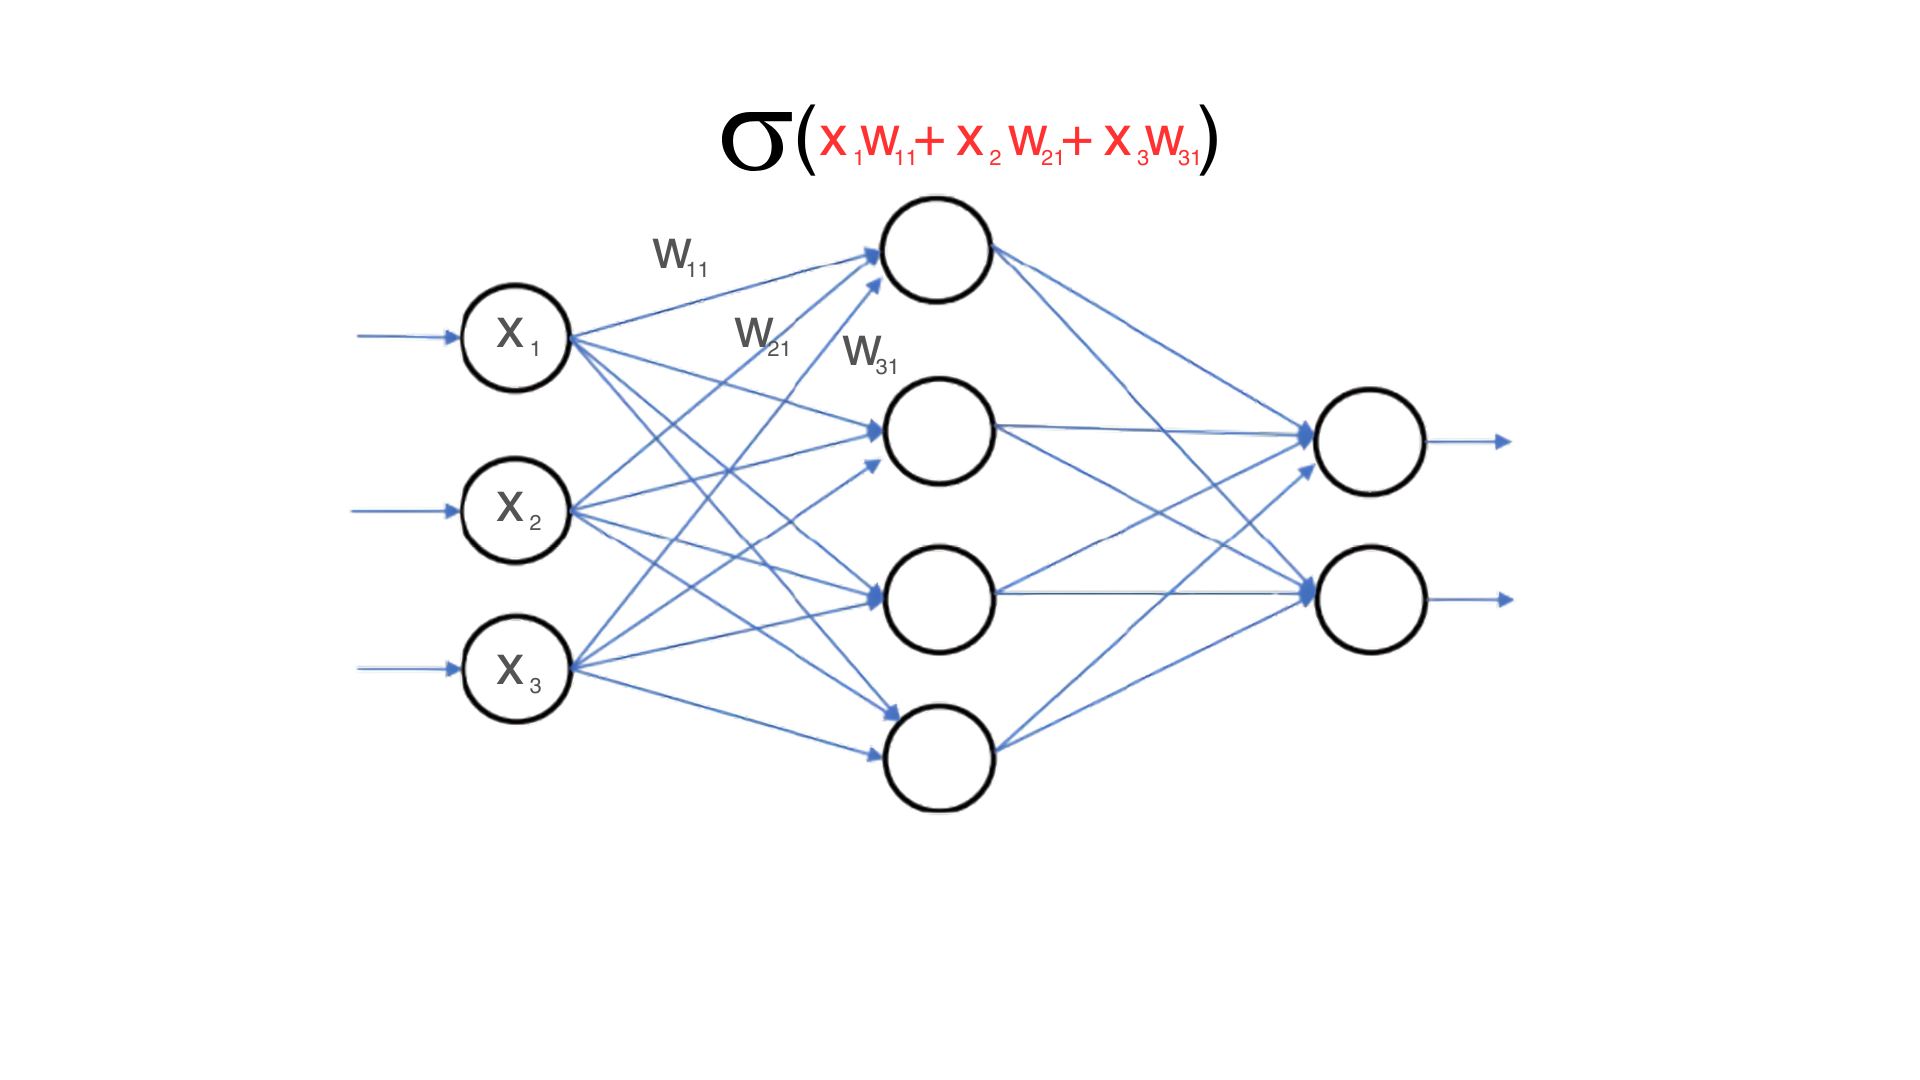
\includegraphics[width=1.3\textwidth]{Neural Network/8.png}
        }
        \captionsetup{labelformat=empty}
    \end{figure}
\end{frame}

\begin{frame}{Neural Networks} 
    \begin{figure}[h]
        \centering
        \makebox[\linewidth]{% ensures centering even if the image is wider than the text width
            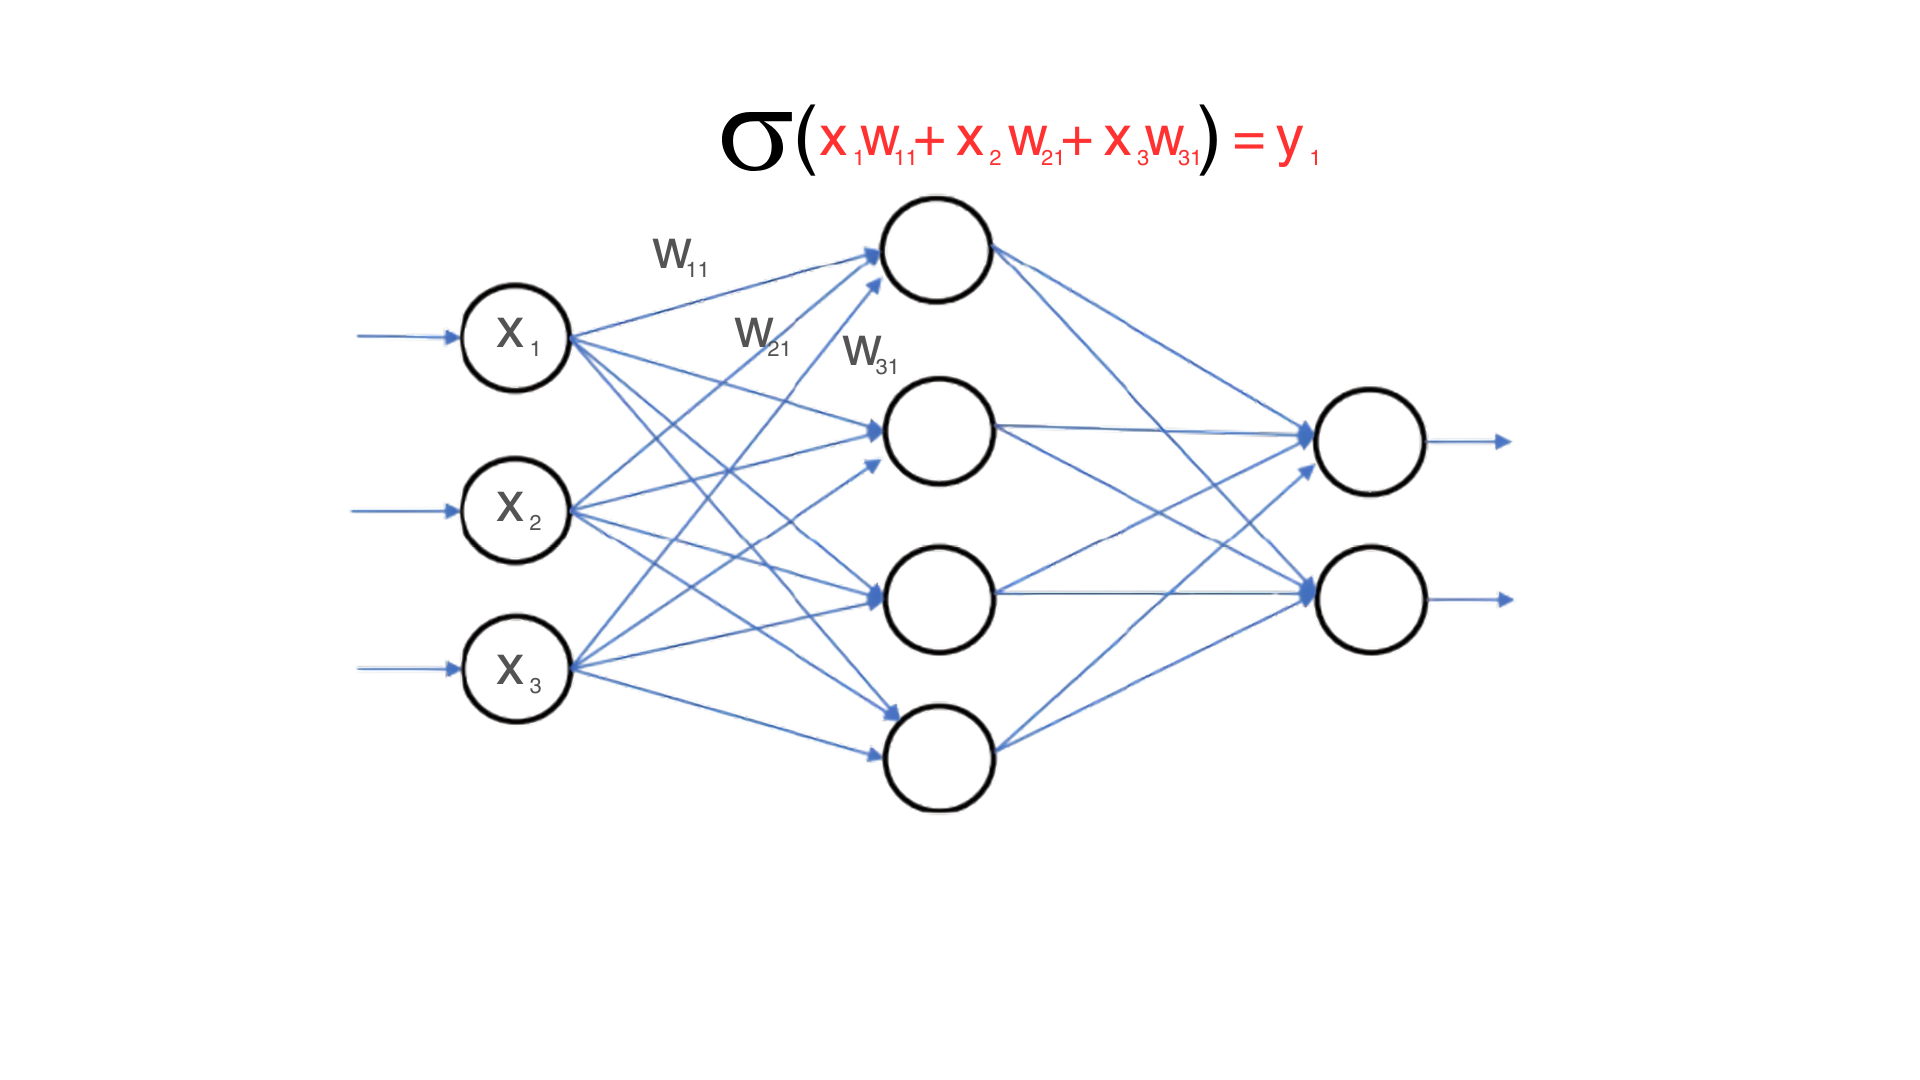
\includegraphics[width=1.3\textwidth]{Neural Network/9.png}
        }
        \captionsetup{labelformat=empty}
    \end{figure}
\end{frame}


\begin{frame}{Neural Networks-Sigmoid Function} 

    \[
    \displaystyle \sigma(w_{11}x_1 + w_{21}x_2 + w_{31}x_3) = \frac{1}{1 + e^{-(w_{11}x_1 + w_{21}x_2 + w_{31}x_3)}}
    \]
    \begin{figure}[h]
        \centering
        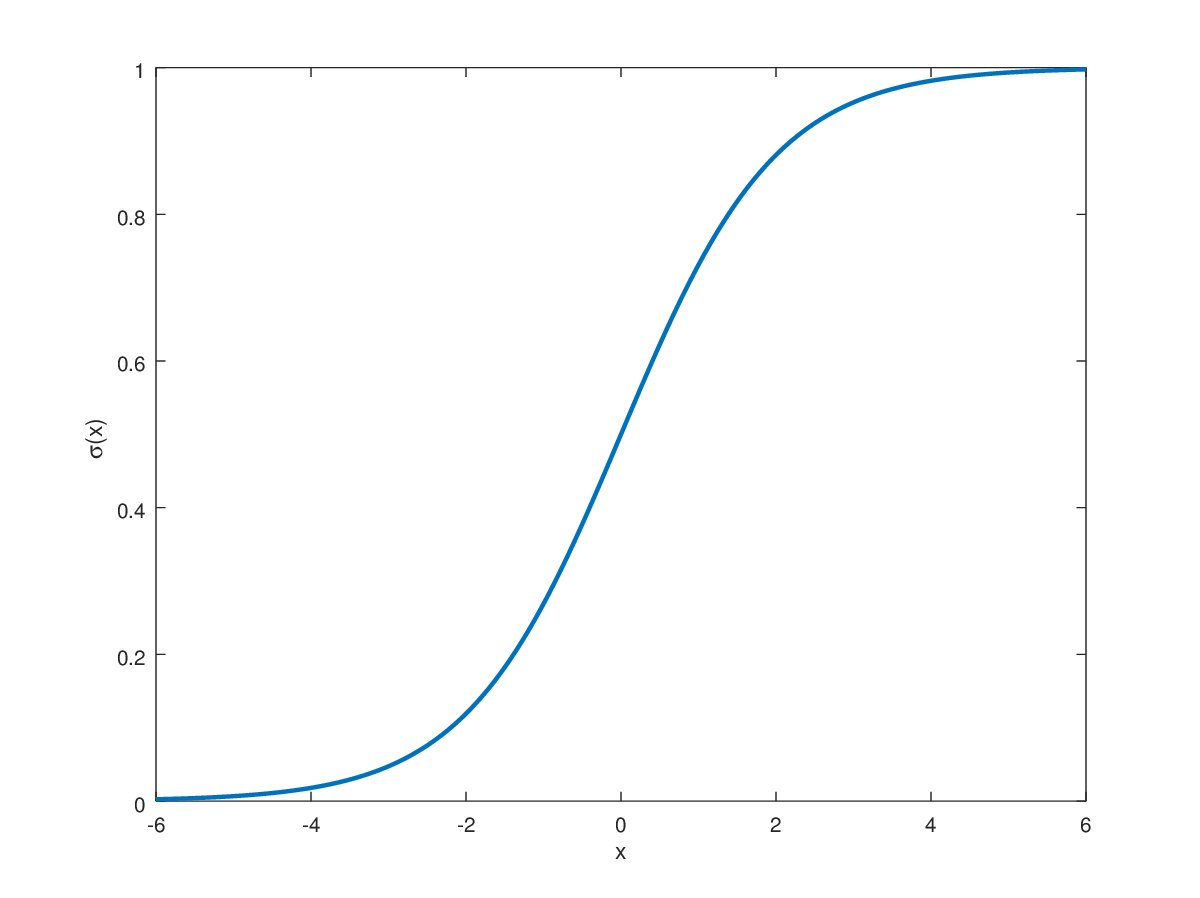
\includegraphics[width=0.75\textwidth]{Neural Network/sigmoid_function.png} % Replace with your image file name
        \captionsetup{labelformat=empty}
    \end{figure}
\end{frame}

\begin{frame}{Neural Networks} 
    \begin{figure}[h]
        \centering
        \makebox[\linewidth]{% ensures centering even if the image is wider than the text width
            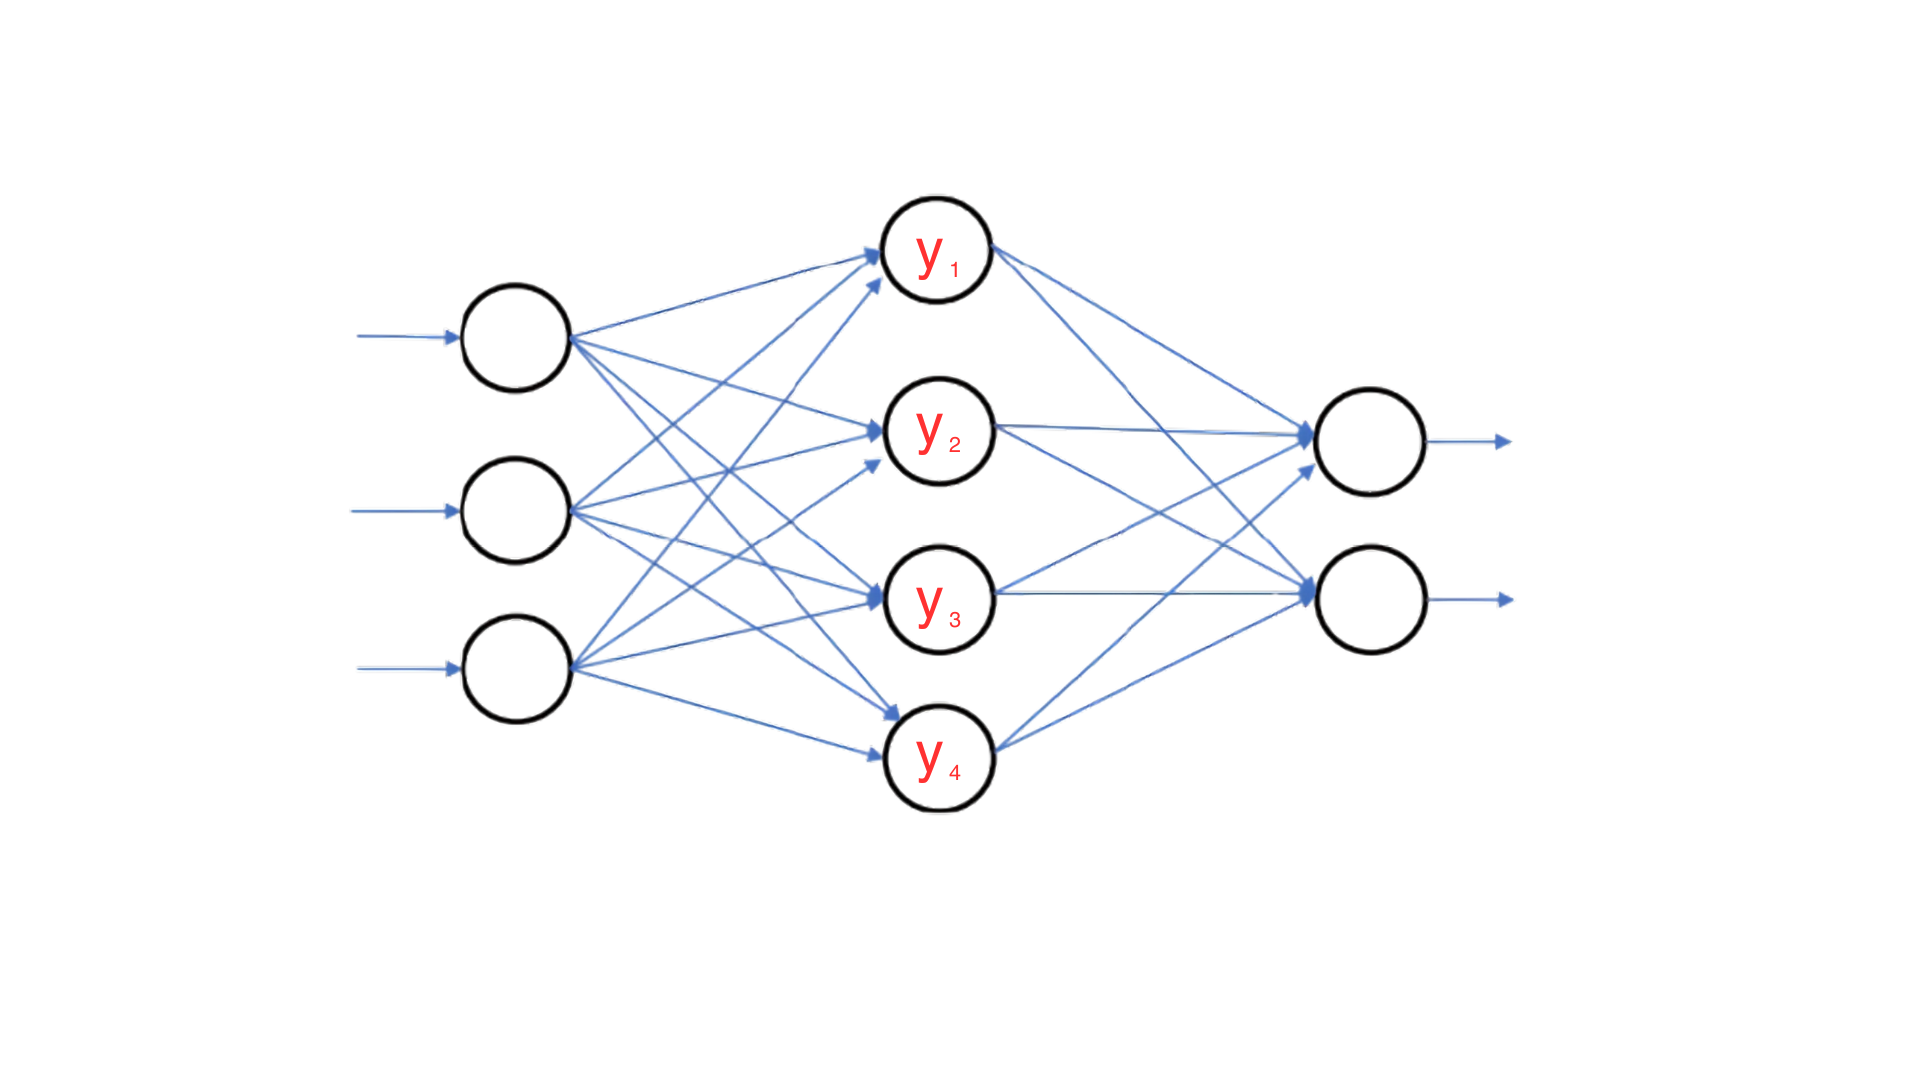
\includegraphics[width=1.3\textwidth]{Neural Network/10.png}
        }
        \captionsetup{labelformat=empty}
    \end{figure}
\end{frame}




\begin{frame}{Neural Network Training}
    \begin{block}{Neural Network Backpropagation}
    This algorithm computes gradients of the loss function with respect to each weight by applying the chain rule. For a neuron output \( a = \sigma(z) \), where \( z = \sum_j w_j y_j + b \), the gradient is:
\[
\frac{\partial \mathcal{L}}{\partial w_i} = \frac{\partial \mathcal{L}}{\partial a} \cdot \frac{\partial a}{\partial y} \cdot \frac{\partial y}{\partial w_i}
\]
Once the gradients are calculated, the weights are updated using:
\[
w^{(t+1)}_i= w^{(t)}_i - \eta \frac{\partial \mathcal{L}}{\partial w_i}
\]
where \( \eta \) is the learning rate.

\end{block}
    
\end{frame}

\begin{frame}{GAN Example - Slanted Land} 
    \begin{figure}[h]
        \centering
        \makebox[\linewidth]{% ensures centering even if the image is wider than the text width
            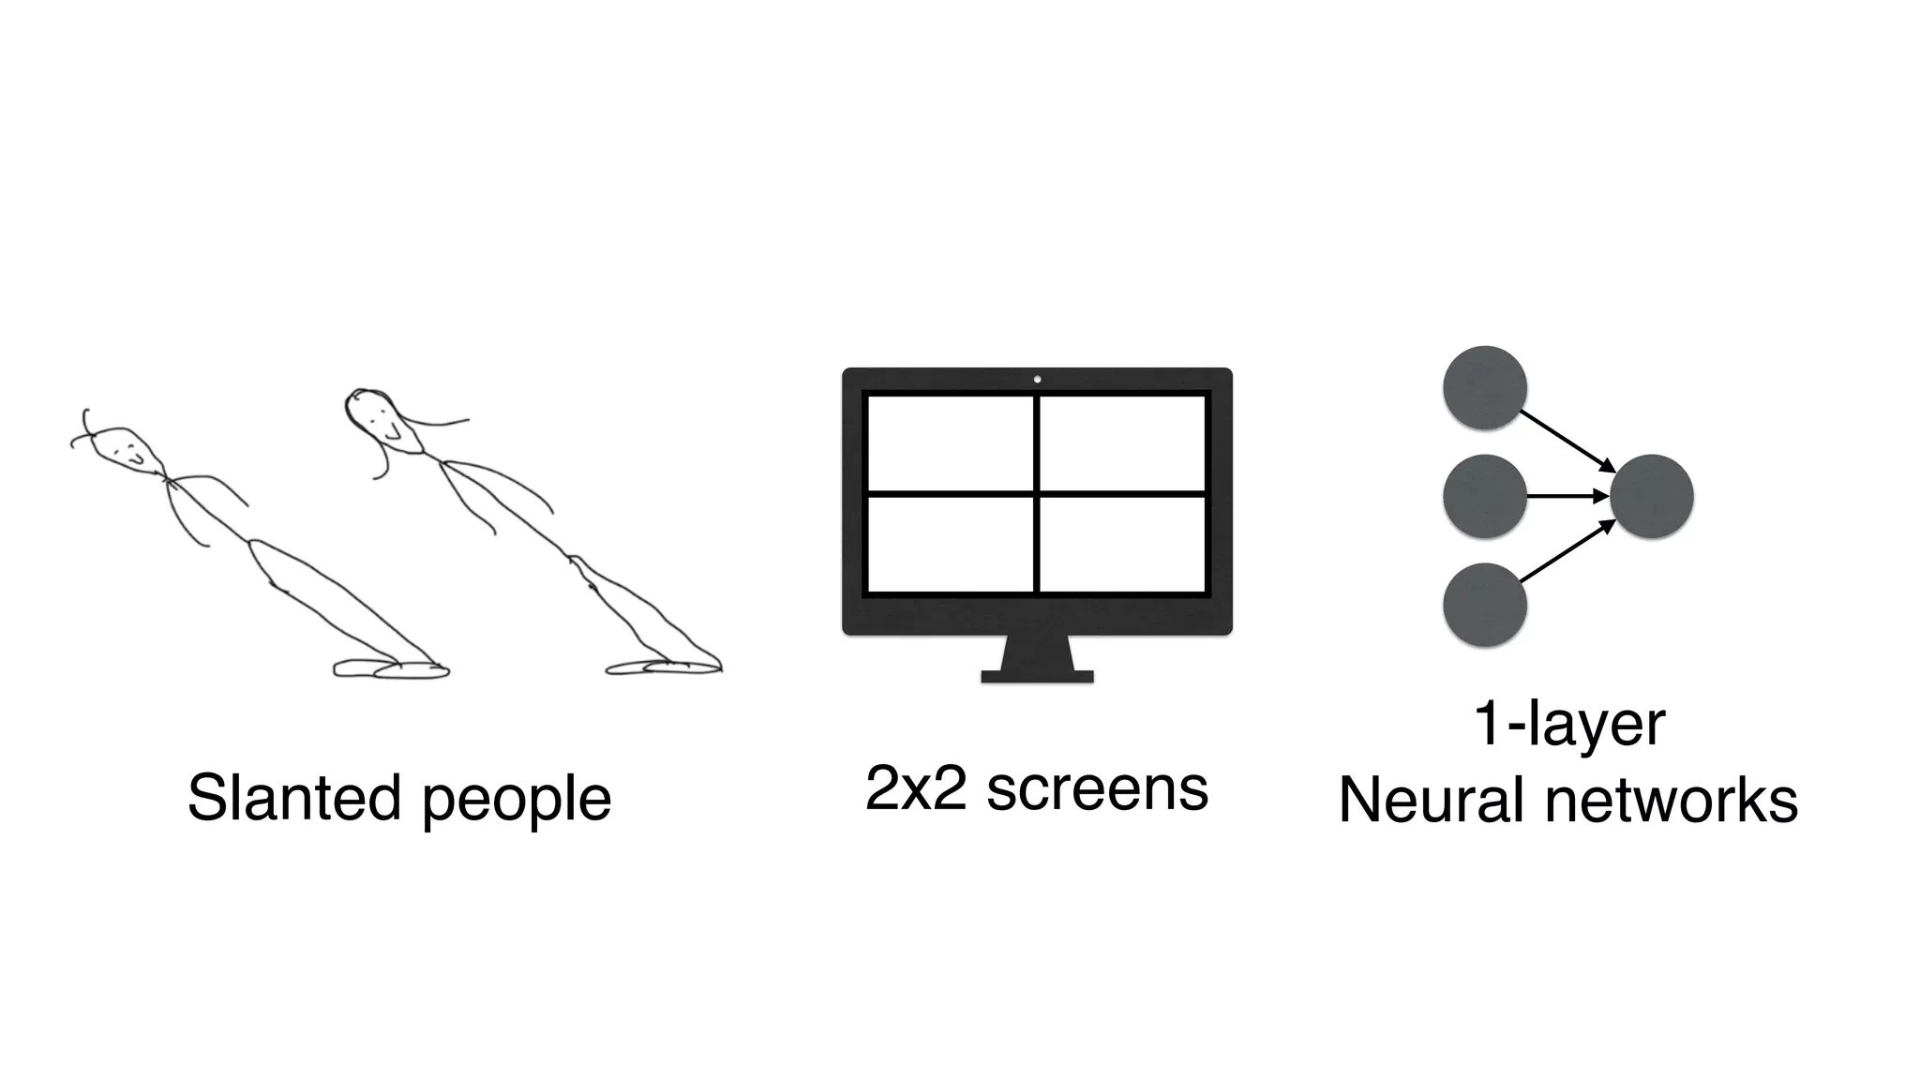
\includegraphics[width=1\textwidth]{Slanted Land/1.jpg}
        }
        \captionsetup{labelformat=empty}
    \end{figure}
\end{frame}

\begin{frame}{Slanted Land - Faces} 
    \begin{figure}[h]
        \centering
        \makebox[\linewidth]{% ensures centering even if the image is wider than the text width
            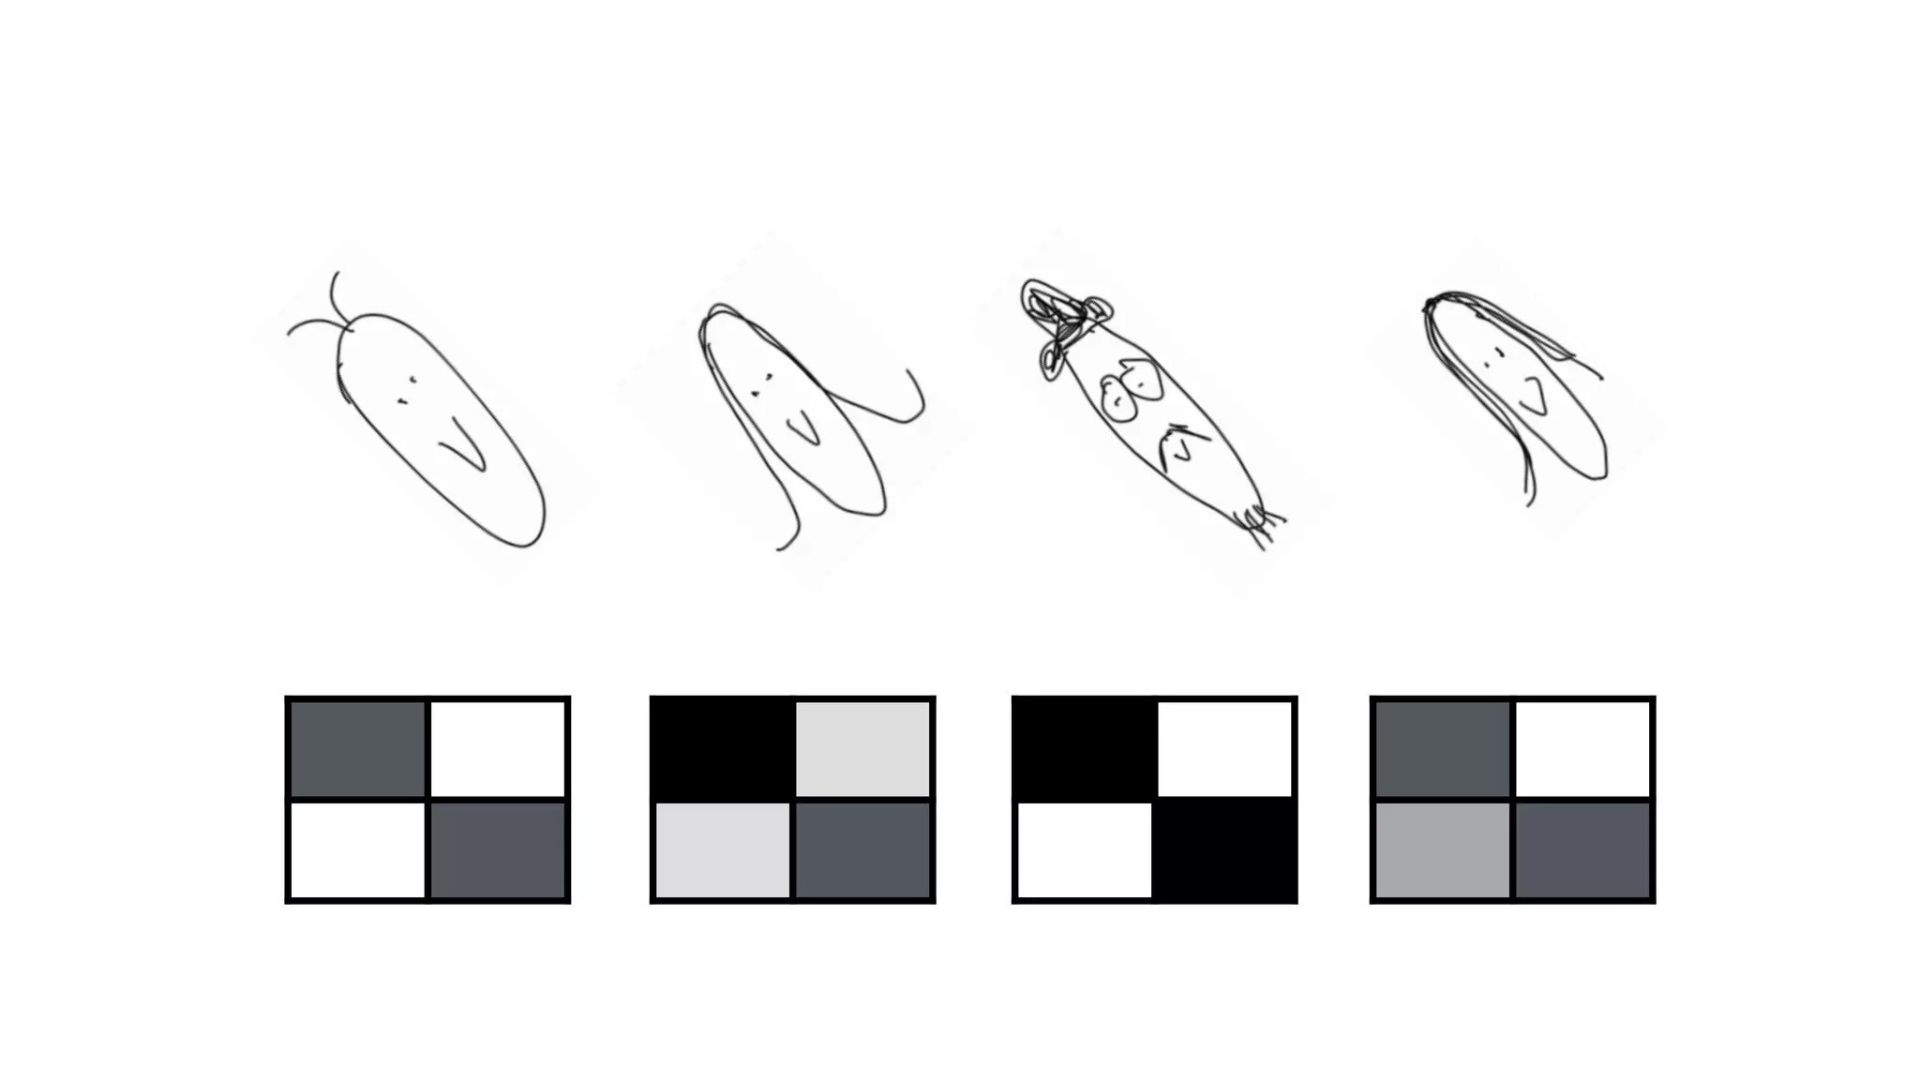
\includegraphics[width=1\textwidth]{Slanted Land/2.jpg}
        }
        \captionsetup{labelformat=empty}
    \end{figure}
\end{frame}

\begin{frame}{Slanted Land - Noises} 
    \begin{figure}[h]
        \centering
        \makebox[\linewidth]{% ensures centering even if the image is wider than the text width
            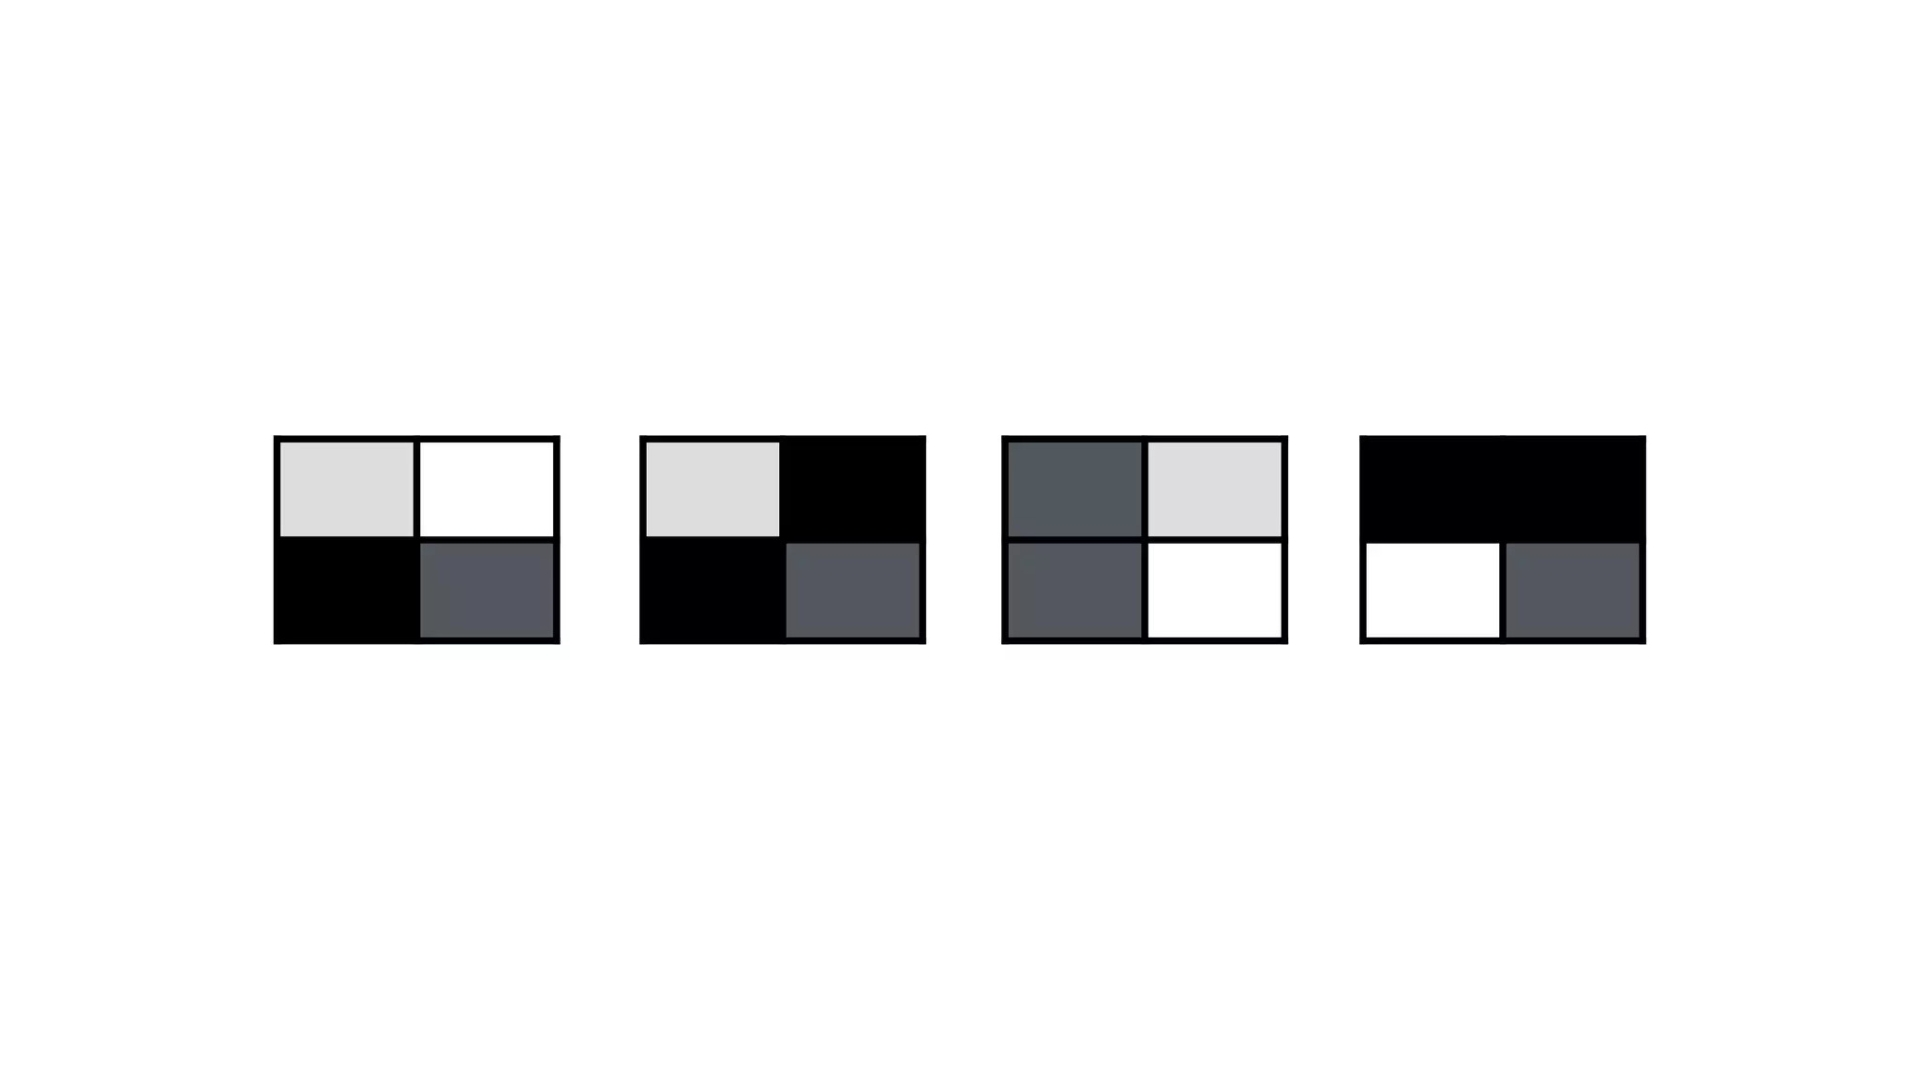
\includegraphics[width=1\textwidth]{Slanted Land/3.jpg}
        }
        \captionsetup{labelformat=empty}
    \end{figure}
\end{frame}

\begin{frame}{Slanted Land - Faces and Noises} 
    \begin{figure}[h]
        \centering
        \makebox[\linewidth]{% ensures centering even if the image is wider than the text width
            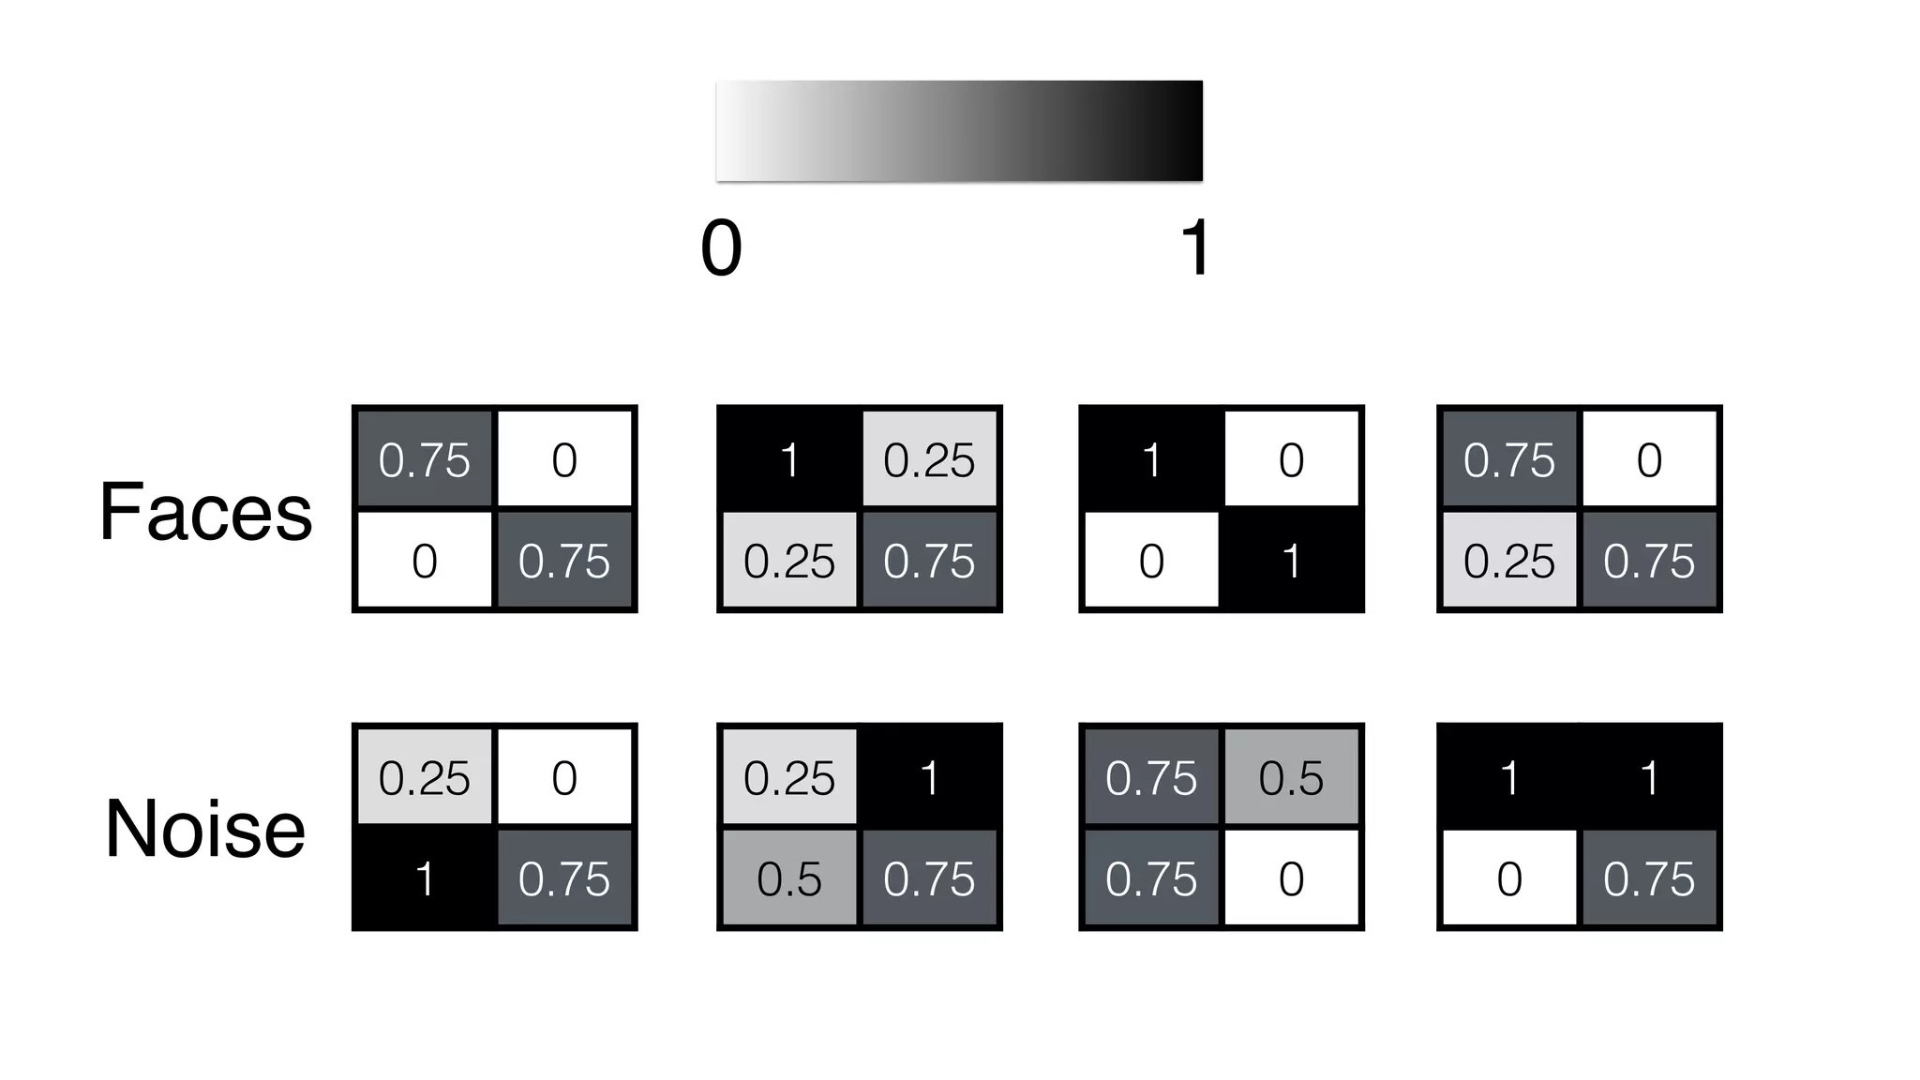
\includegraphics[width=1\textwidth]{Slanted Land/4.jpg}
        }
        \captionsetup{labelformat=empty}
    \end{figure}
\end{frame}

\begin{frame}{Slanted Land - Faces and Noises} 
    \begin{figure}[h]
        \centering
        \makebox[\linewidth]{% ensures centering even if the image is wider than the text width
            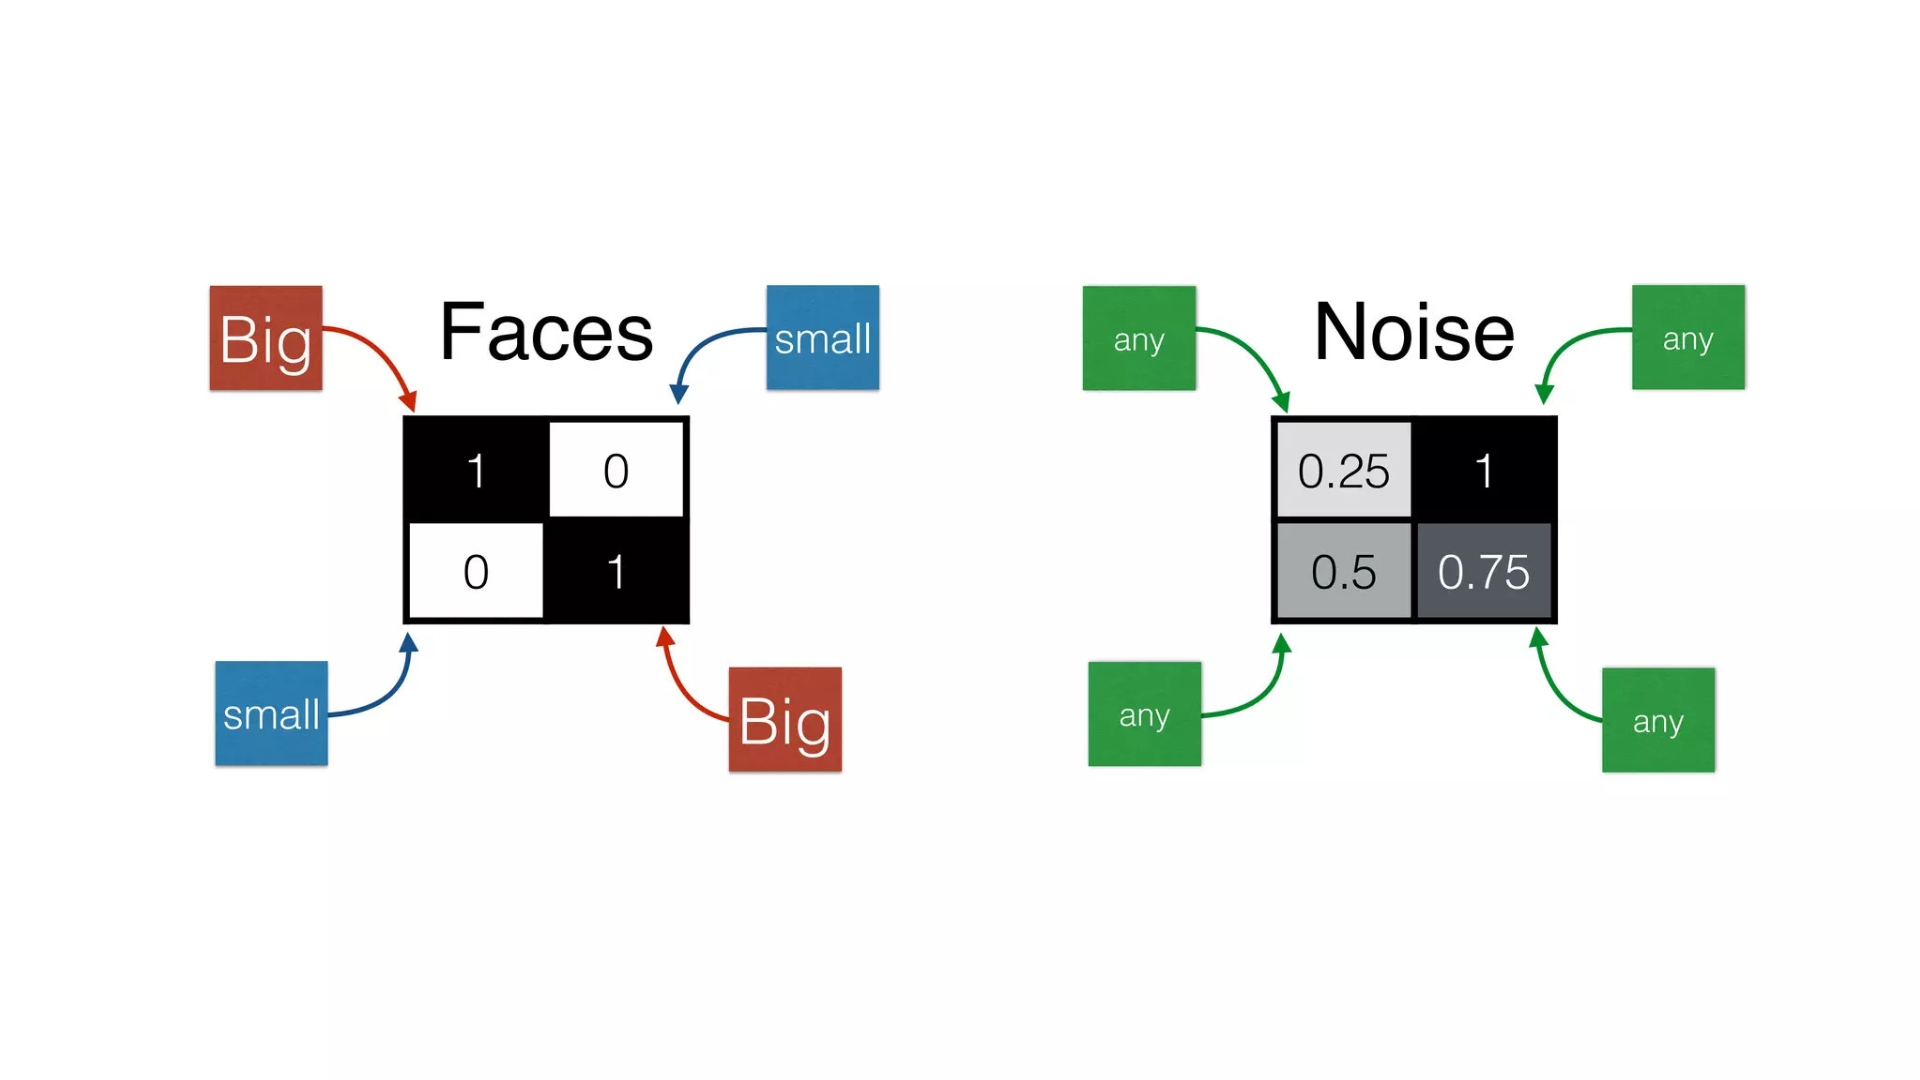
\includegraphics[width=1\textwidth]{Slanted Land/5.jpg}
        }
        \captionsetup{labelformat=empty}
    \end{figure}
\end{frame}

\begin{frame}{Building Discriminator} 
    \begin{figure}[h]
        \centering
        \makebox[\linewidth]{% ensures centering even if the image is wider than the text width
            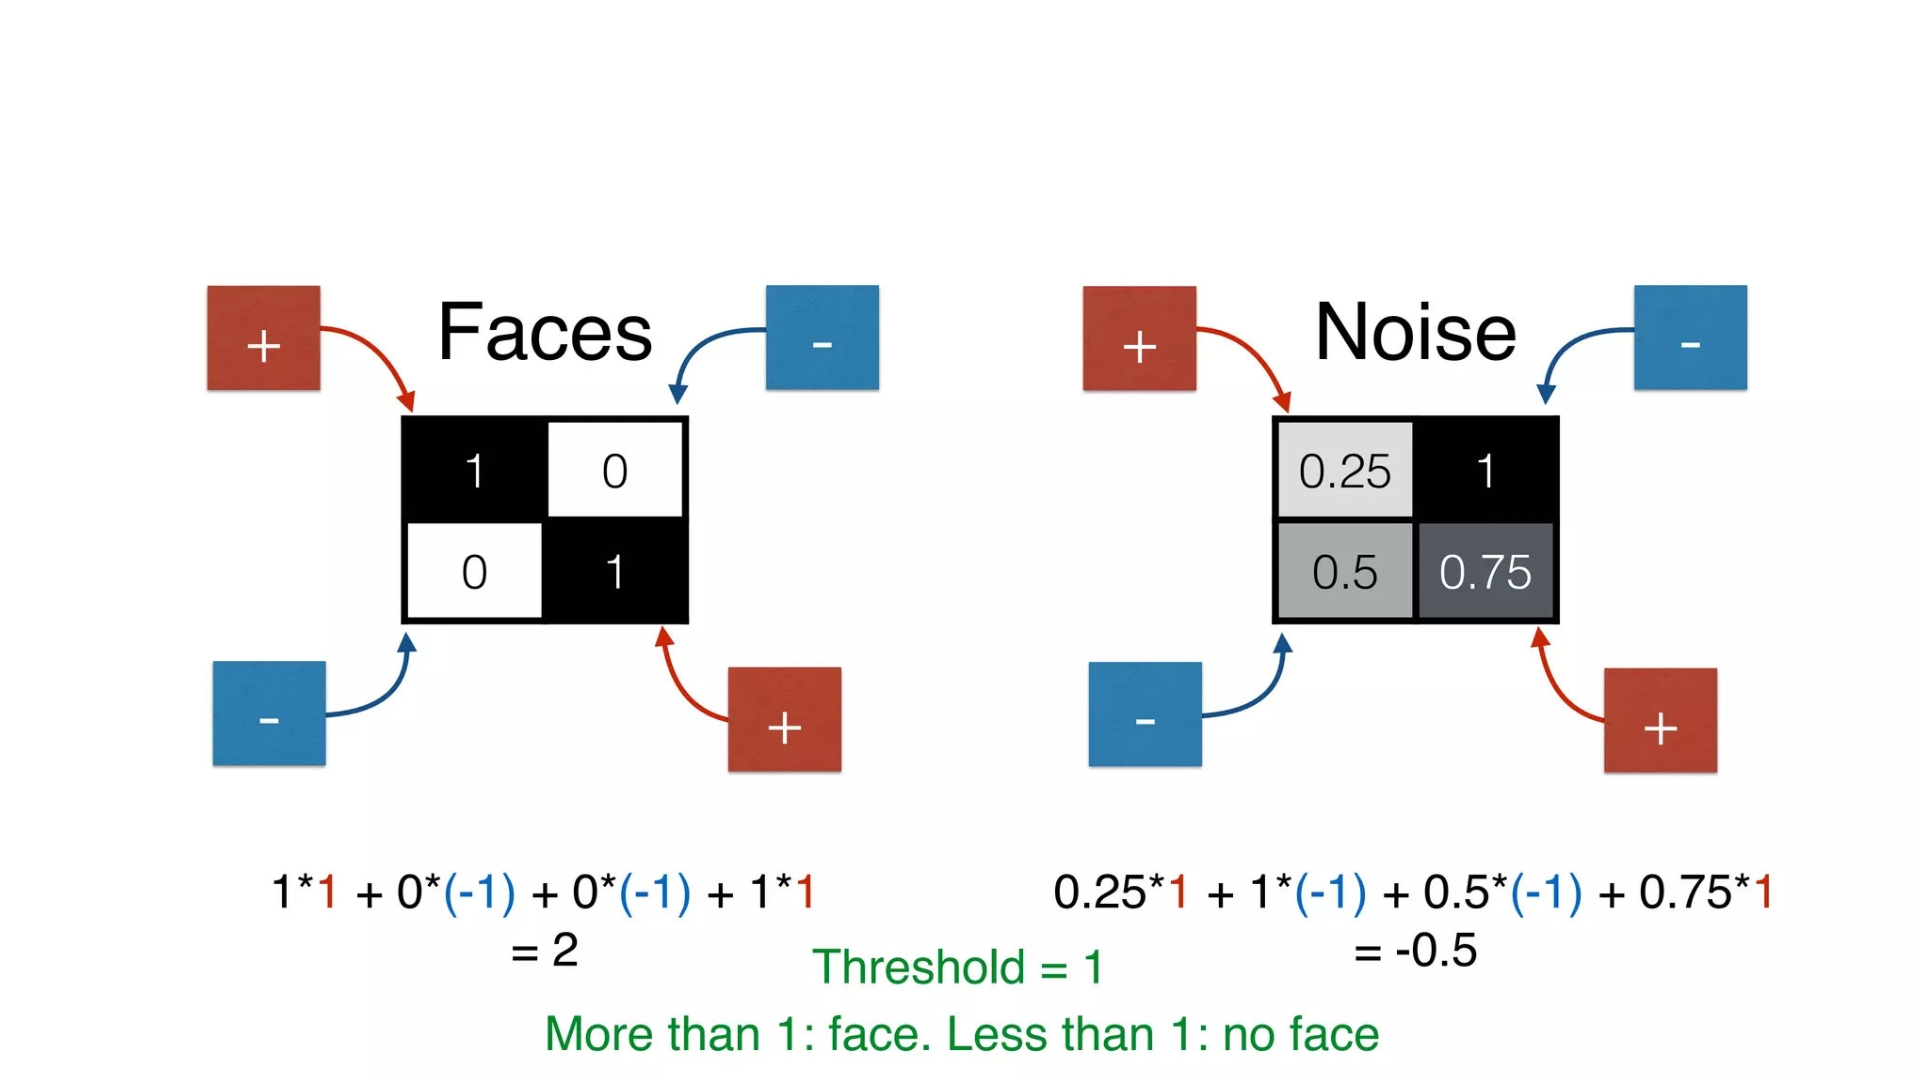
\includegraphics[width=1\textwidth]{Slanted Land/6.jpg}
        }
        \captionsetup{labelformat=empty}
    \end{figure}
\end{frame}

\begin{frame}{Building Discriminator} 
    \begin{figure}[h]
        \centering
        \makebox[\linewidth]{% ensures centering even if the image is wider than the text width
            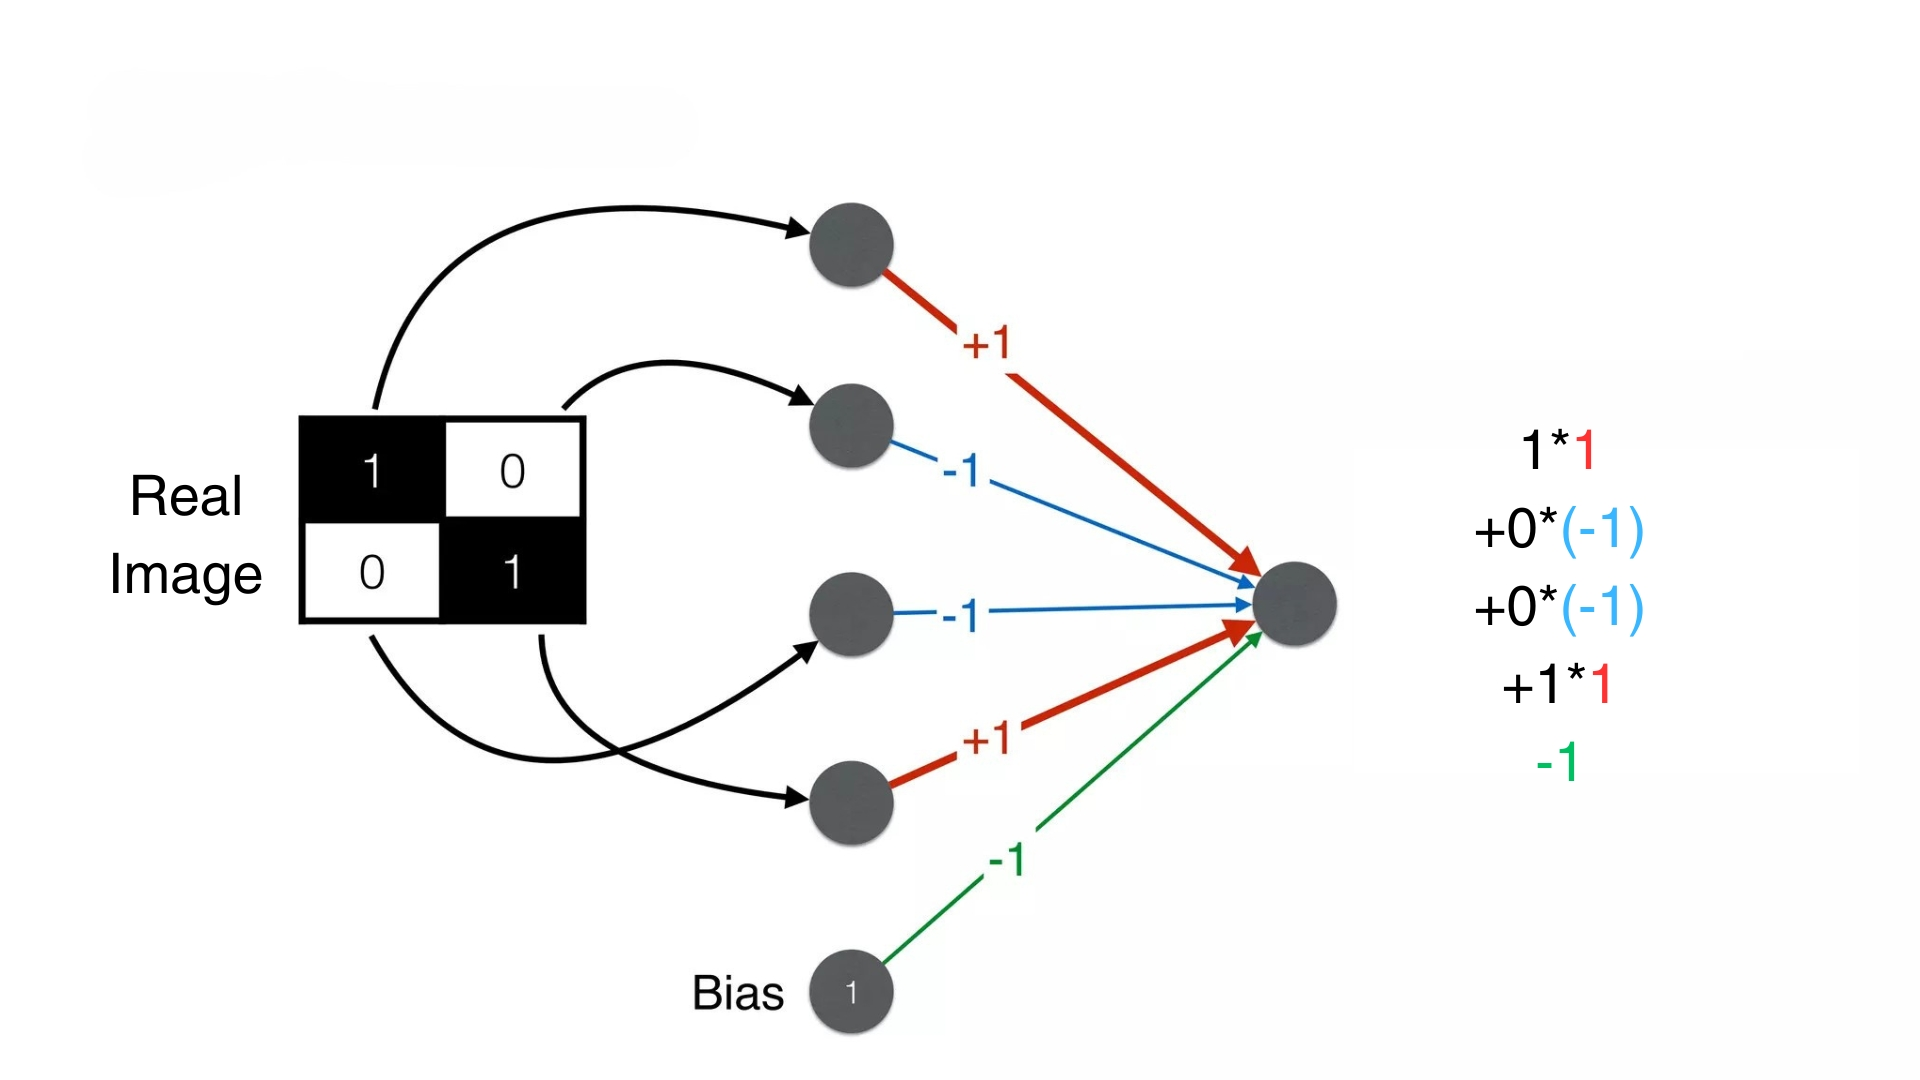
\includegraphics[width=1\textwidth]{Slanted Land/7.jpg}
        }
        \captionsetup{labelformat=empty}
    \end{figure}
\end{frame}

\begin{frame}{Building Discriminator} 
    \begin{figure}[h]
        \centering
        \makebox[\linewidth]{% ensures centering even if the image is wider than the text width
            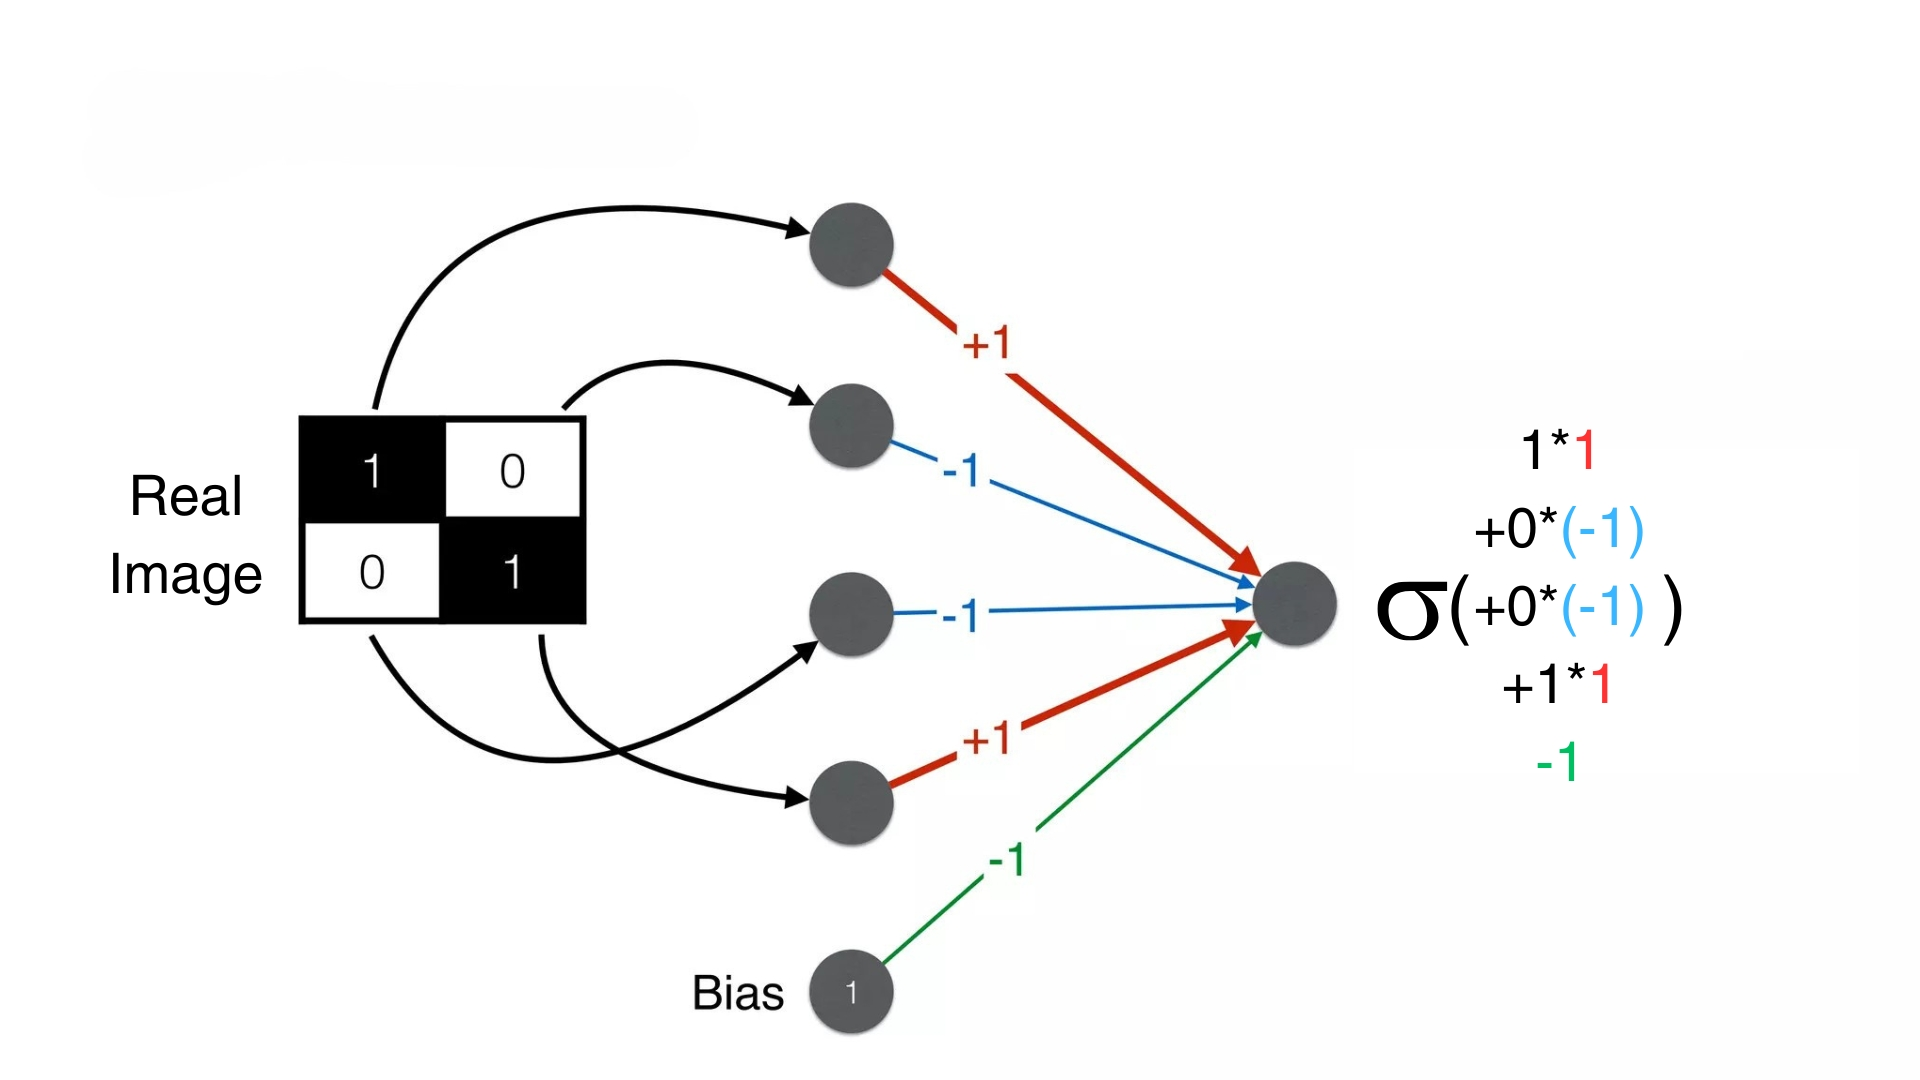
\includegraphics[width=1\textwidth]{Slanted Land/8.jpg}
        }
        \captionsetup{labelformat=empty}
    \end{figure}
\end{frame}

\begin{frame}{Building Discriminator} 
    \begin{figure}[h]
        \centering
        \makebox[\linewidth]{% ensures centering even if the image is wider than the text width
            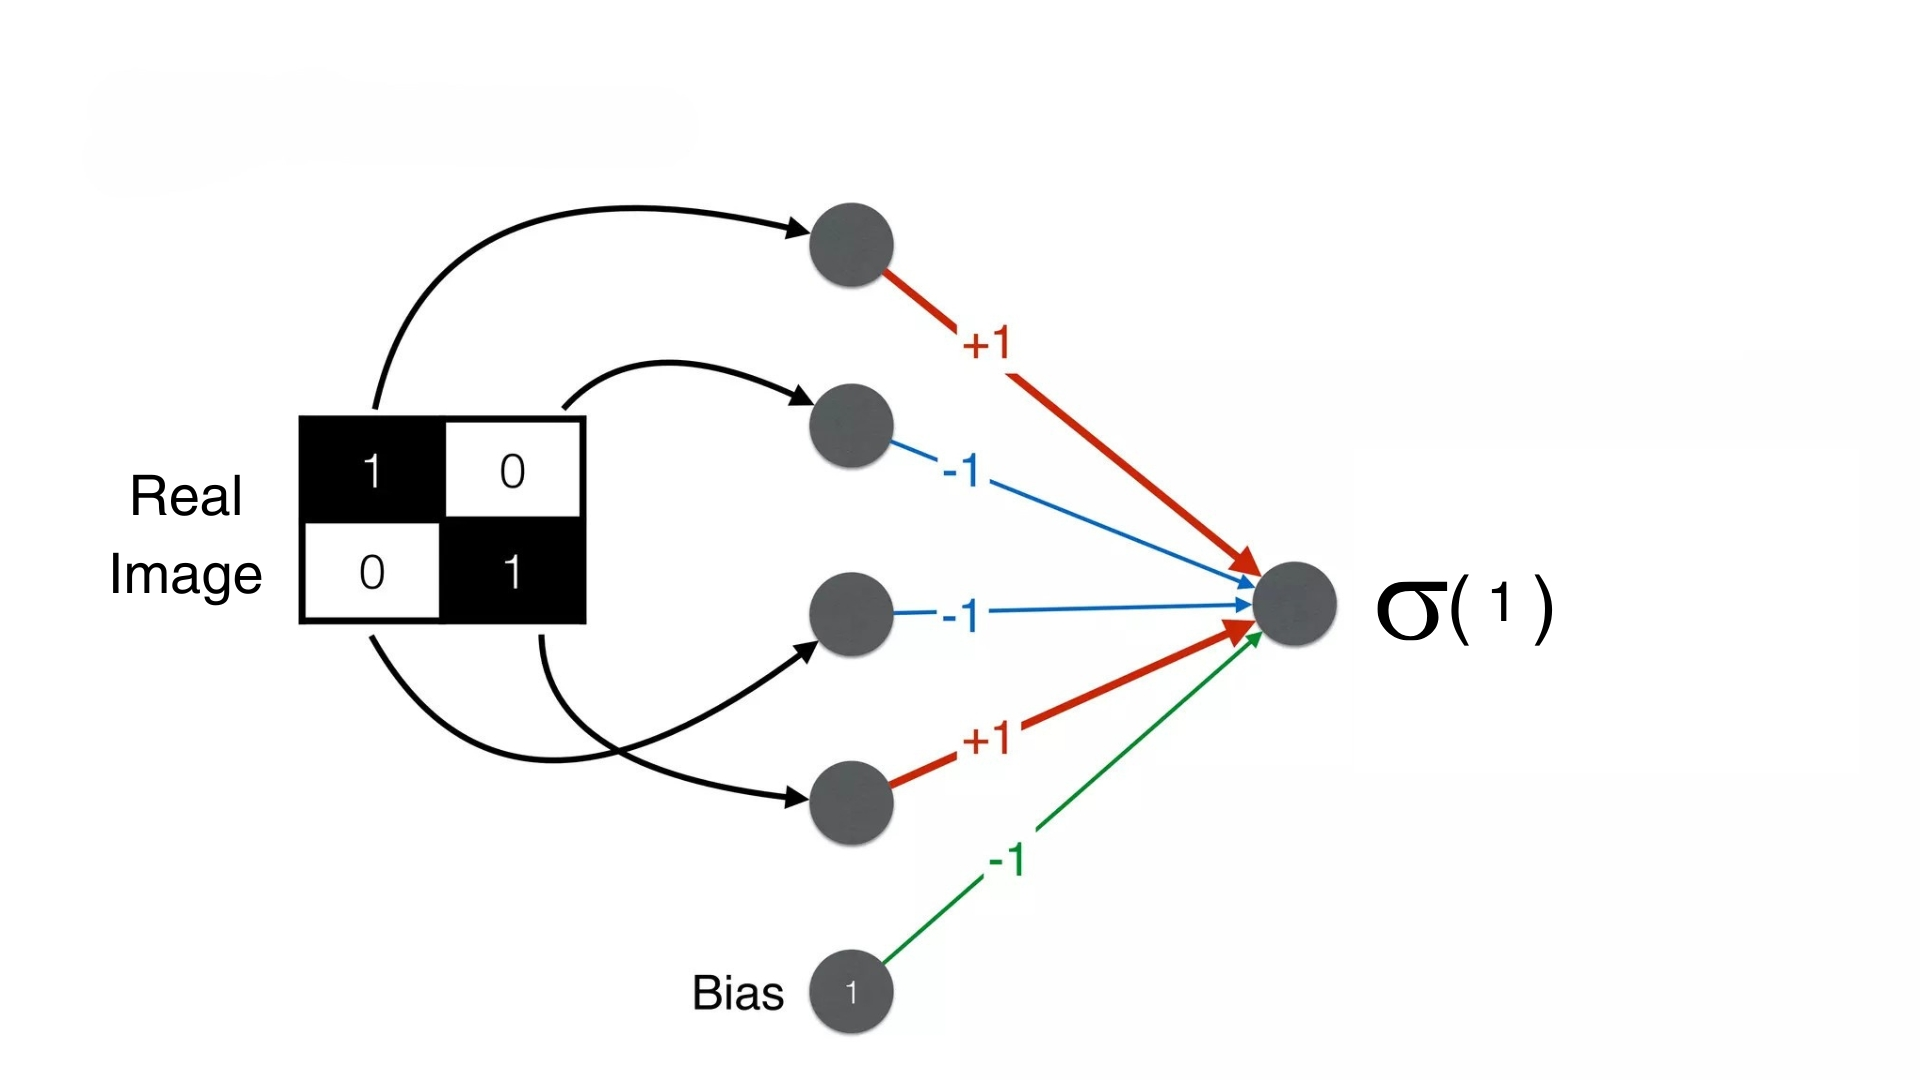
\includegraphics[width=1\textwidth]{Slanted Land/9.jpg}
        }
        \captionsetup{labelformat=empty}
    \end{figure}
\end{frame}

\begin{frame}{Building Discriminator} 
    \begin{figure}[h]
        \centering
        \makebox[\linewidth]{% ensures centering even if the image is wider than the text width
            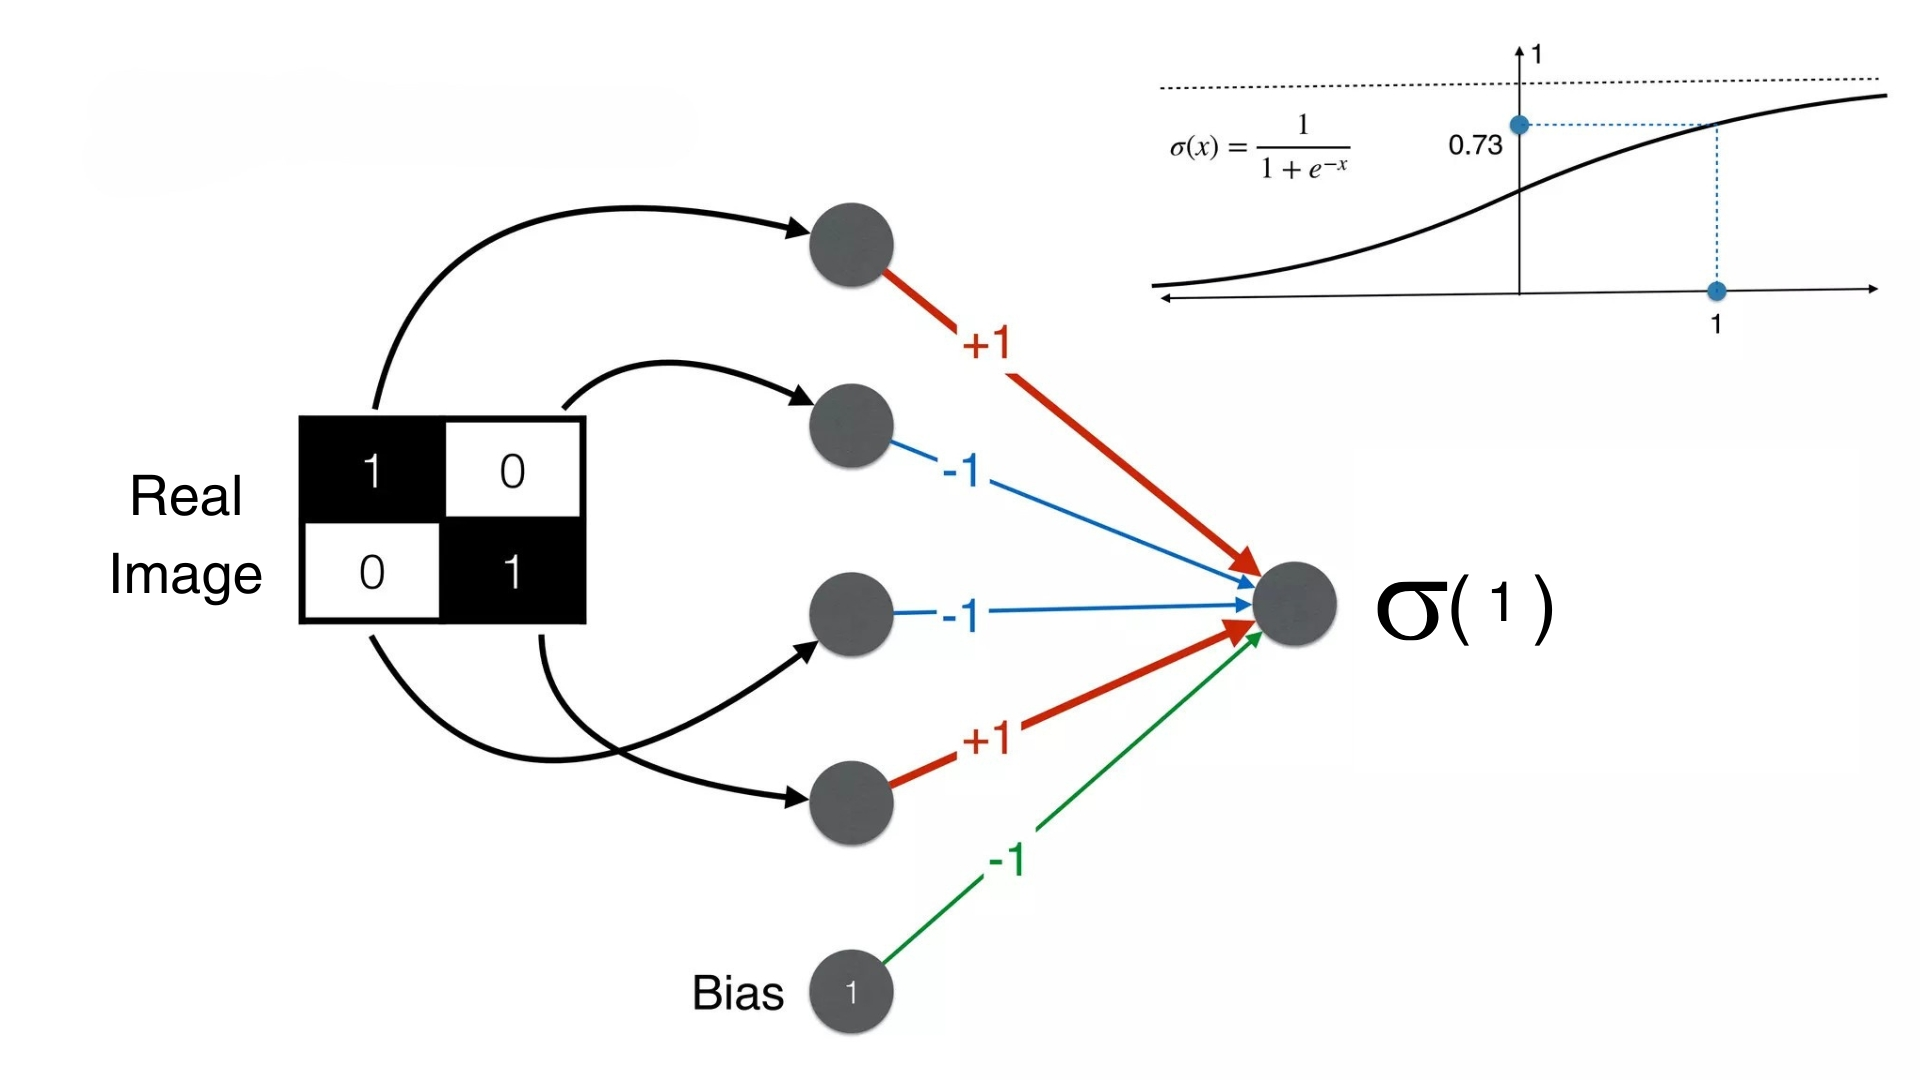
\includegraphics[width=1\textwidth]{Slanted Land/10.jpg}
        }
        \captionsetup{labelformat=empty}
    \end{figure}
\end{frame}


\begin{frame}{Building Discriminator} 
    \begin{figure}[h]
        \centering
        \makebox[\linewidth]{% ensures centering even if the image is wider than the text width
            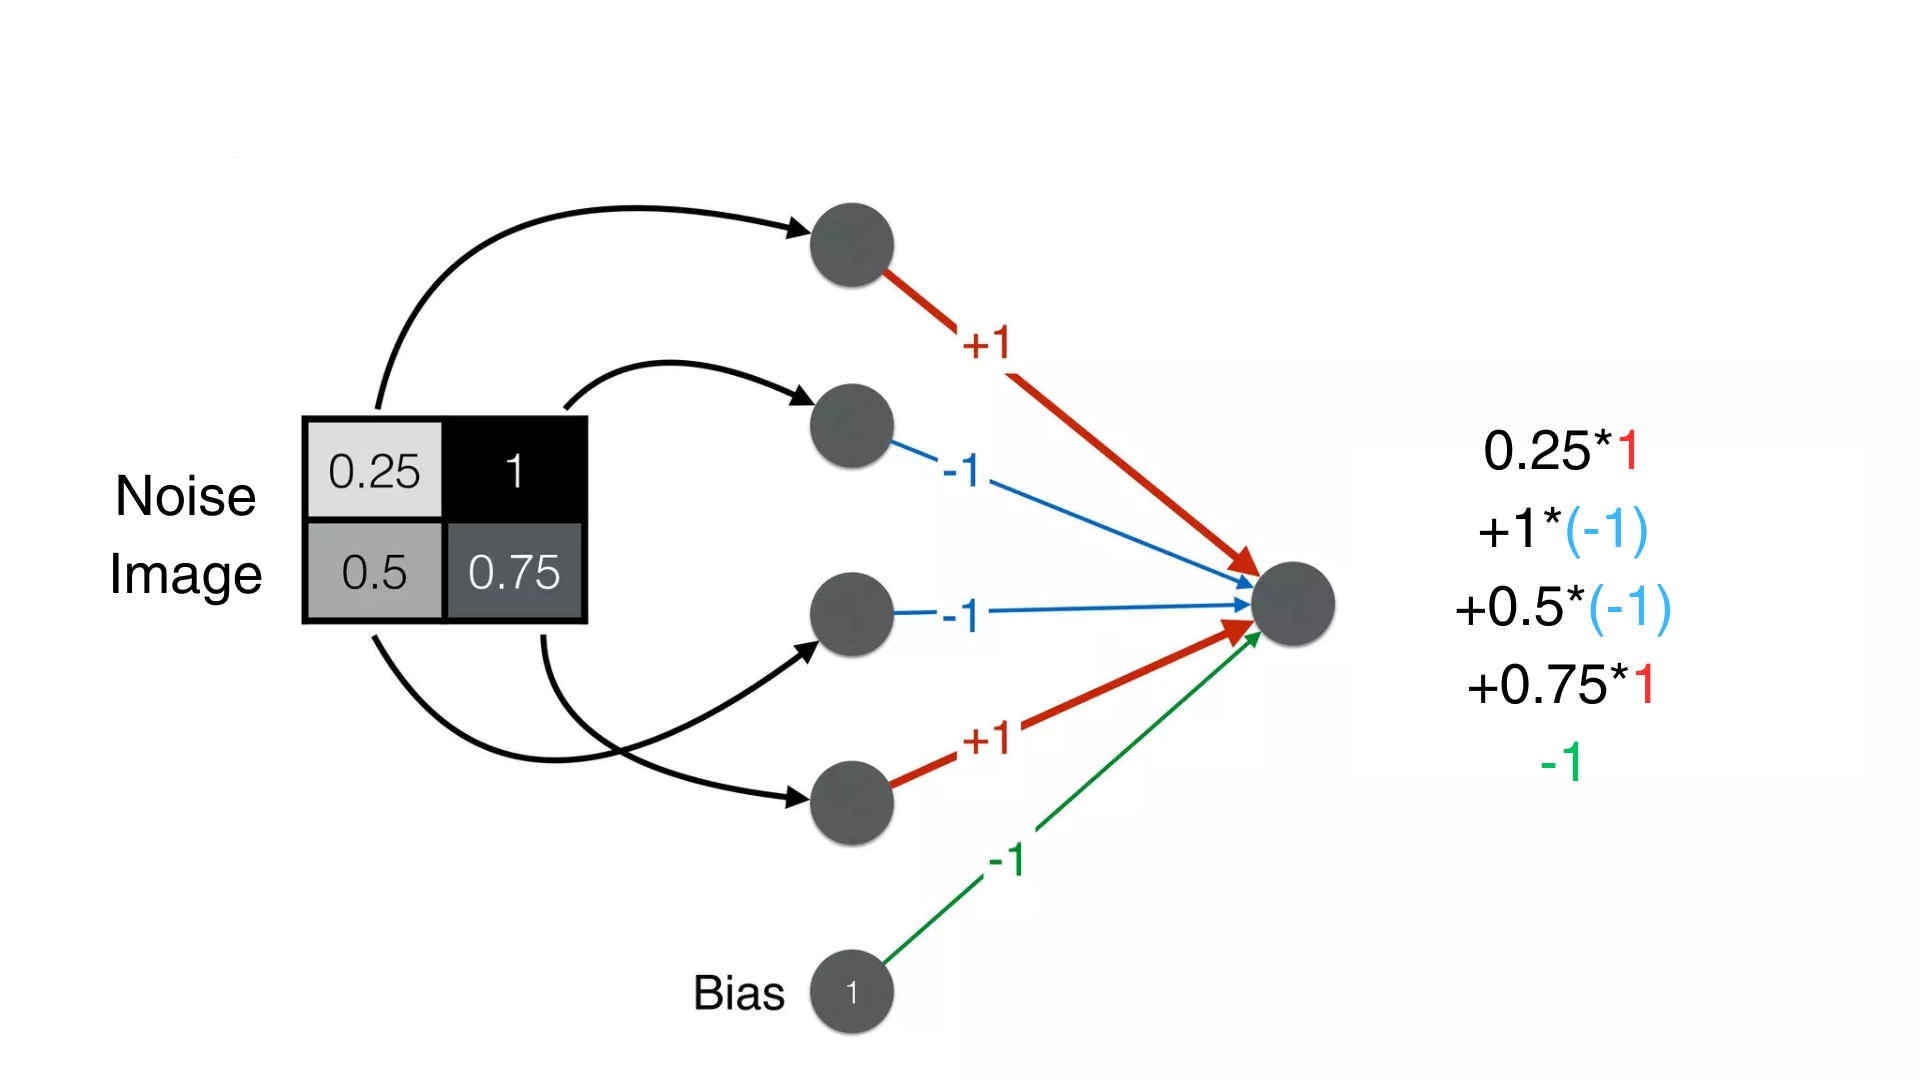
\includegraphics[width=1\textwidth]{Slanted Land/11.jpg}
        }
        \captionsetup{labelformat=empty}
    \end{figure}
\end{frame}

\begin{frame}{Building Discriminator} 
    \begin{figure}[h]
        \centering
        \makebox[\linewidth]{% ensures centering even if the image is wider than the text width
            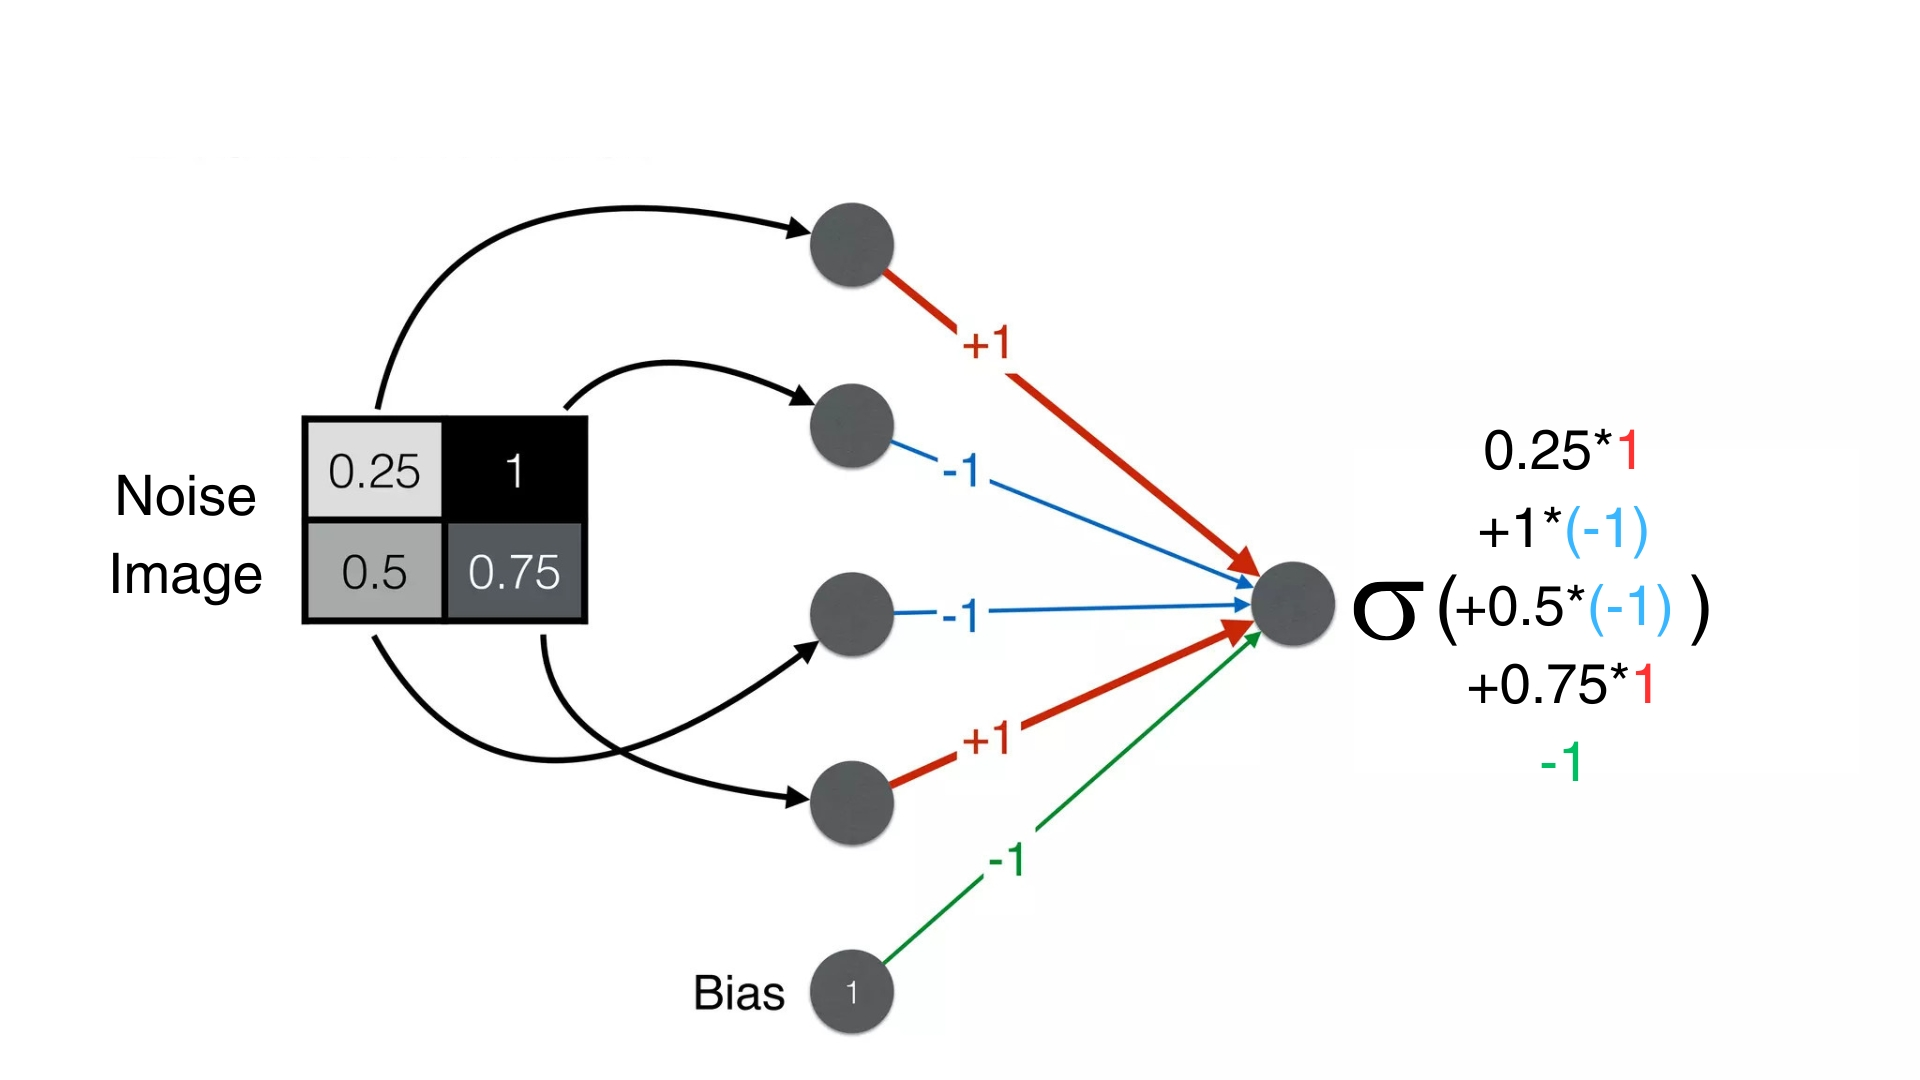
\includegraphics[width=1\textwidth]{Slanted Land/12.jpg}
        }
        \captionsetup{labelformat=empty}
    \end{figure}
\end{frame}

\begin{frame}{Building Discriminator} 
    \begin{figure}[h]
        \centering
        \makebox[\linewidth]{% ensures centering even if the image is wider than the text width
            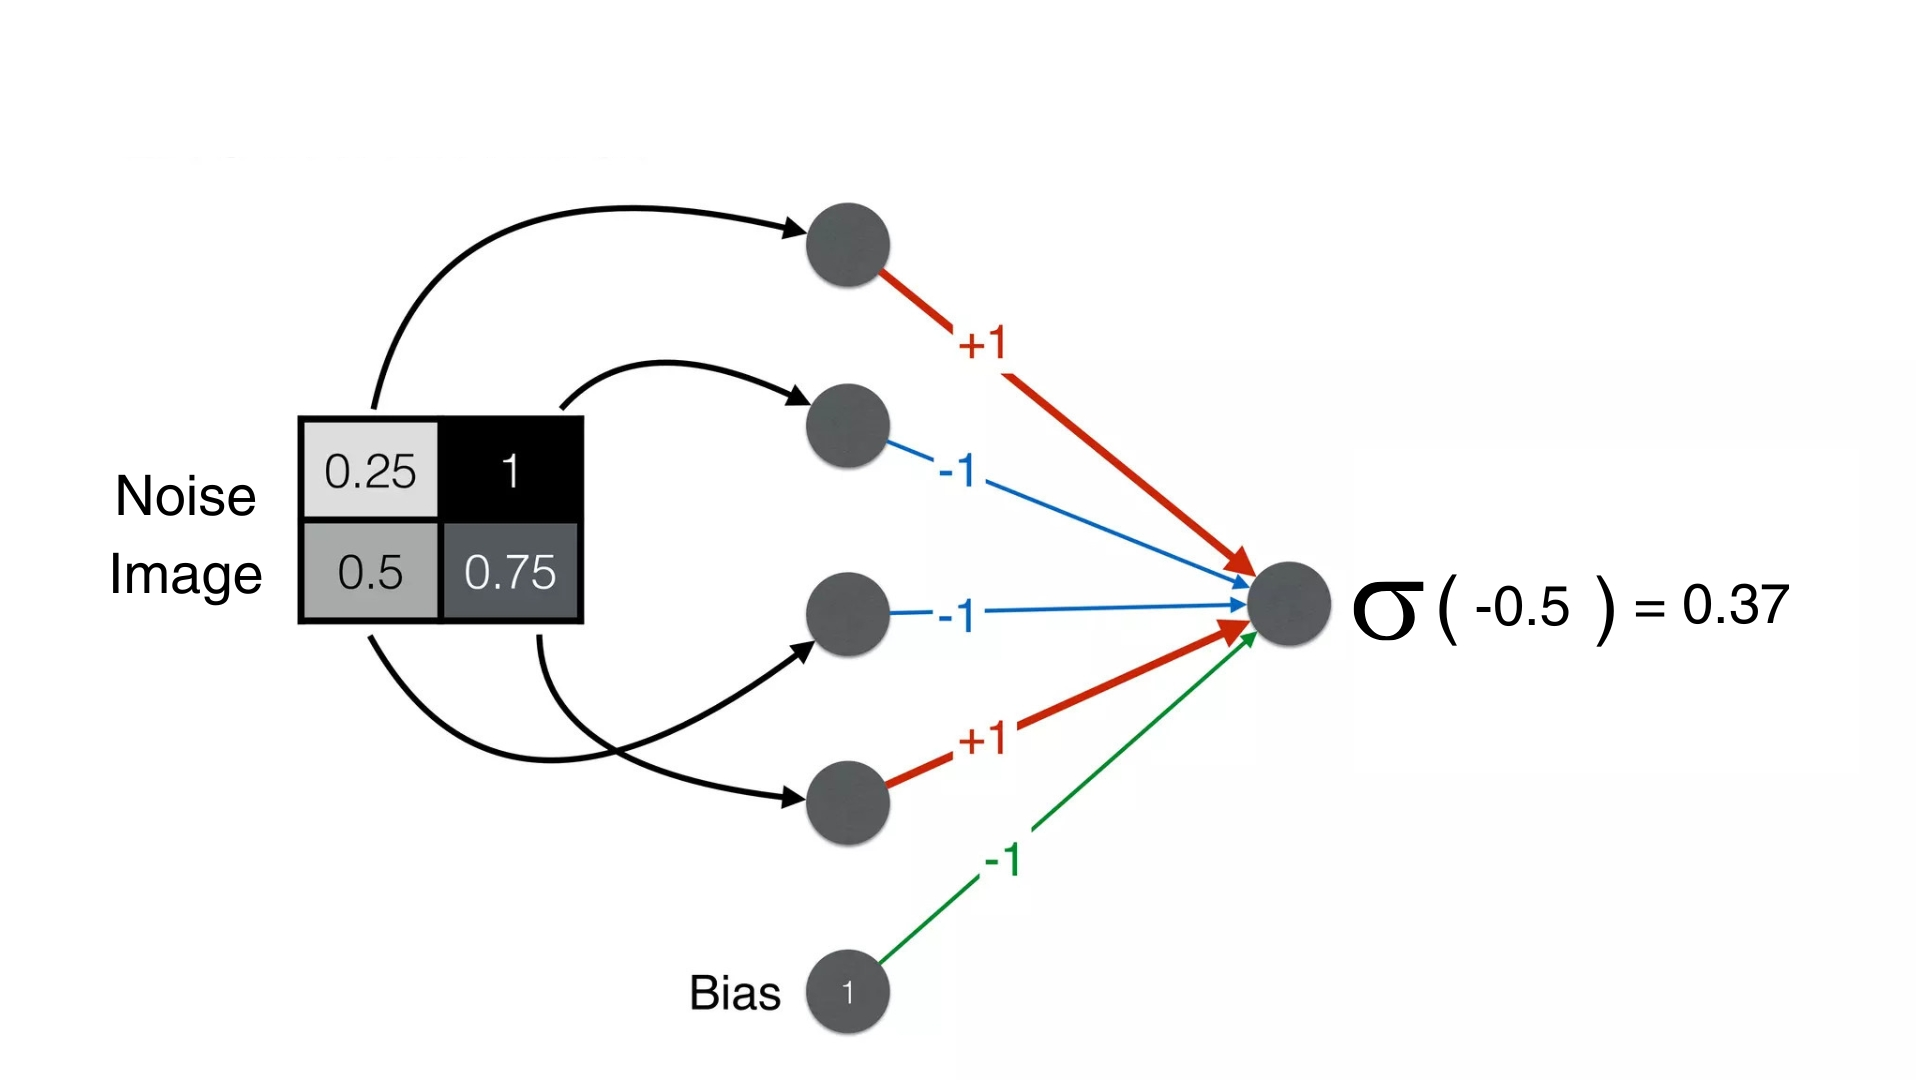
\includegraphics[width=1\textwidth]{Slanted Land/13.jpg}
        }
        \captionsetup{labelformat=empty}
    \end{figure}
\end{frame}

\begin{frame}{Building Generator} 
    \begin{figure}[h]
        \centering
        \makebox[\linewidth]{% ensures centering even if the image is wider than the text width
            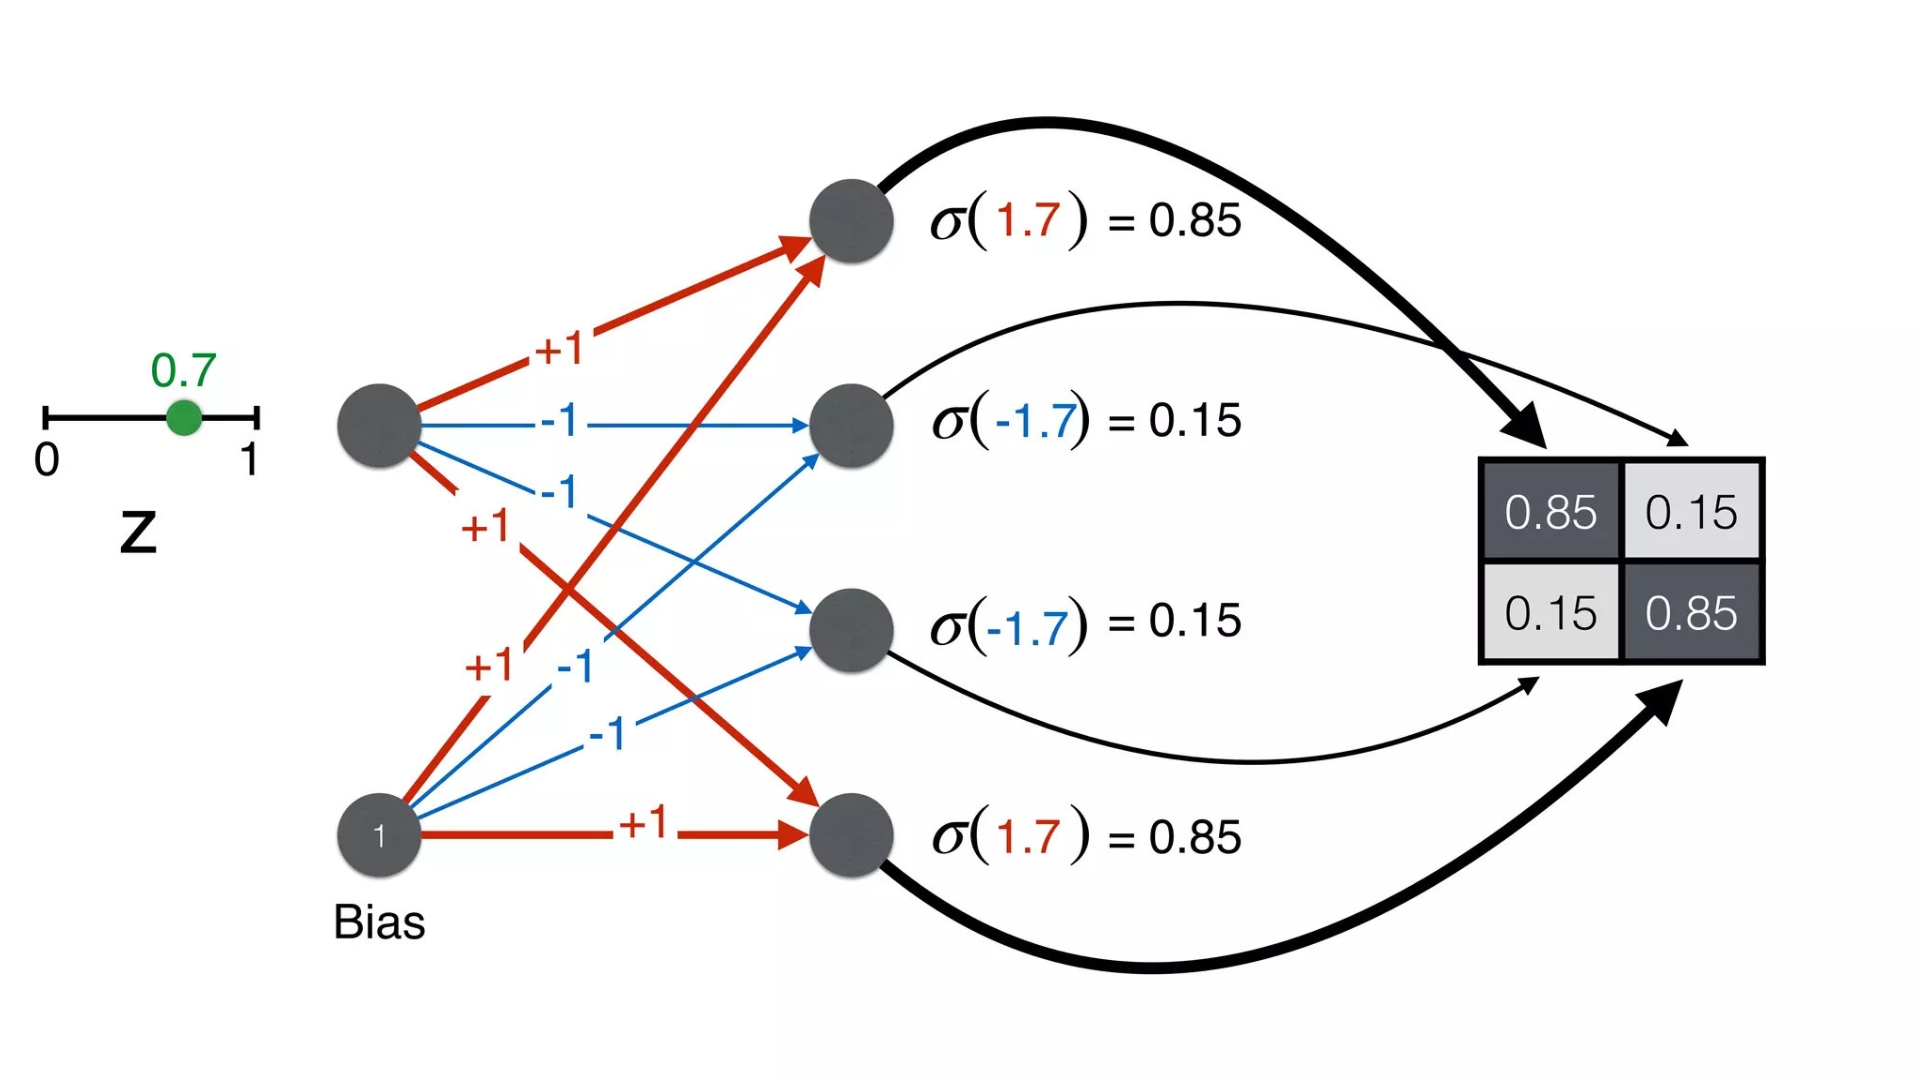
\includegraphics[width=1\textwidth]{Slanted Land/14.jpg}
        }
        \captionsetup{labelformat=empty}
    \end{figure}
\end{frame}


\begin{frame}{Log Loss Error}


\begin{flushleft}
    \Large Label: 1 \\
    \Large Prediction: 0.1 
\end{flushleft}

\end{frame}

\begin{frame}{Log Loss Error}
    

\begin{flushleft}
    \Large Label: 1 \\
    \Large Prediction: 0.1 \hfill Error: large 
\end{flushleft}


\end{frame}

\begin{frame}{Log Loss Error}
    

\begin{flushleft}
    \Large Label: 1 \\
    \Large Prediction: 0.1 \hfill Error: large \hfill 
\end{flushleft}

\begin{flushleft}
    \Large Label: 1\\
    \Large Prediction: 0.9 \hfill
\end{flushleft}
\end{frame}

\begin{frame}{Log Loss Error}
    \begin{center}
    \Large Error = $-\ln(\text{prediction})$
\end{center}

\begin{flushleft}
    \Large Label: 1 \\
    \Large Prediction: 0.1 \hfill Error: large 
\end{flushleft}

\begin{flushleft}
    \Large Label: 1\\
    \Large Prediction: 0.9\hfill Error: small
\end{flushleft}
\end{frame}

\begin{frame}{Log Loss Error}
    \begin{center}
    \Large Error = $-\ln(\text{prediction})$
\end{center}

\begin{flushleft}
    \Large Label: 1 \\
    \Large Prediction: 0.1 \hfill Error: large \hfill $-\ln(0.1) = 2.3$
\end{flushleft}

\begin{flushleft}
    \Large Label: 1\\
    \Large Prediction: 0.9\hfill Error: small \hfill $-\ln(0.9) = 0.1$
\end{flushleft}
\end{frame}

\begin{frame}{Log Loss Error}


\begin{flushleft}
    \Large Label: 0 \\
    \Large Prediction: 0.1 
\end{flushleft}

\end{frame}

\begin{frame}{Log Loss Error}
    

\begin{flushleft}
    \Large Label: 0 \\
    \Large Prediction: 0.1 \hfill Error: small 
\end{flushleft}


\end{frame}

\begin{frame}{Log Loss Error}
    

\begin{flushleft}
    \Large Label: 0 \\
    \Large Prediction: 0.1 \hfill Error: small \hfill 
\end{flushleft}

\begin{flushleft}
    \Large Label: 0\\
    \Large Prediction: 0.9 \hfill
\end{flushleft}
\end{frame}

\begin{frame}{Log Loss Error}
    \begin{center}
    \Large Error = $-\ln(1-\text{prediction})$
\end{center}

\begin{flushleft}
    \Large Label: 0 \\
    \Large Prediction: 0.1 \hfill Error: small 
\end{flushleft}

\begin{flushleft}
    \Large Label: 0\\
    \Large Prediction: 0.9\hfill Error: large
\end{flushleft}
\end{frame}

\begin{frame}{Log Loss Error}
    \begin{center}
    \Large Error = $-\ln(1-\text{prediction})$
\end{center}

\begin{flushleft}
    \Large Label: 0 \\
    \Large Prediction: 0.1 \hfill Error: small \hfill $-\ln(0.9) = 0.1$
\end{flushleft}

\begin{flushleft}
    \Large Label: 0\\
    \Large Prediction: 0.9\hfill Error: large \hfill $-\ln(0.1) = 2.3$
\end{flushleft}
\end{frame}

\begin{frame}{GAN Objective Function}

\begin{block}{GAN Objective Function}
\[
\min_G \max_D V(D, G) = \mathbb{E}_{\mathbf{x} \sim p_{\text{data}}(\mathbf{x})} [\log D(\mathbf{x})] + 
\mathbb{E}_{\mathbf{z} \sim p_{\mathbf{z}}(\mathbf{z})} [\log (1 - D(G(\mathbf{z})))].
\]
\end{block}
    
\end{frame}

\begin{frame}{Loss Function Optimization}
\[\mathbb{E}_{\mathbf{x} \sim p_{\text{data}}(\mathbf{x})} [\log D(\mathbf{x})]\]
    \begin{figure}[h]
        \centering
        \makebox[\linewidth]{% ensures centering even if the image is wider than the text width
            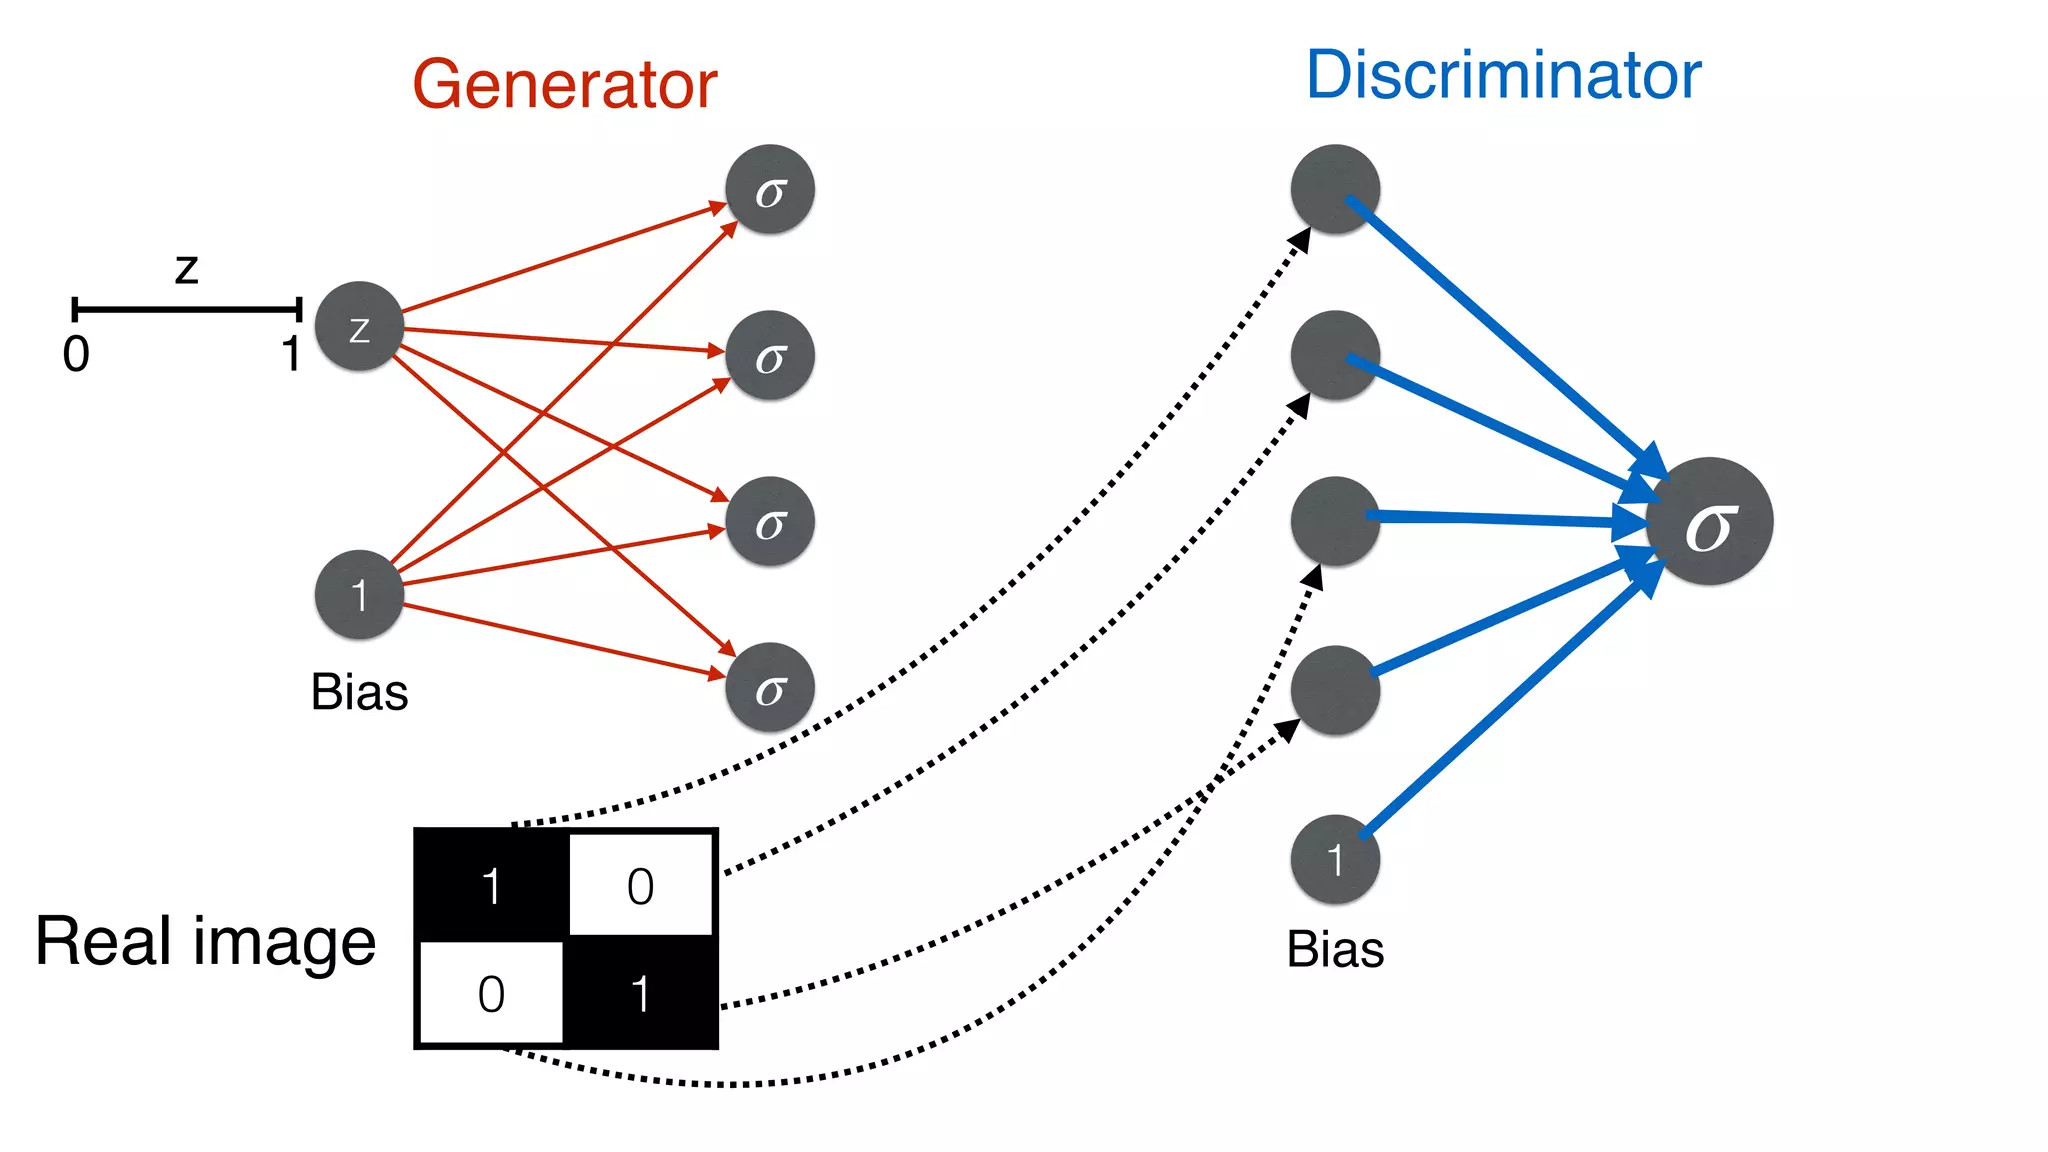
\includegraphics[width=1\textwidth]{Slanted Land/slide_39.jpg}
        }
        \captionsetup{labelformat=empty}
    \end{figure}   
\end{frame}

\begin{frame}{Loss Function Optimization}
\[\mathbb{E}_{\mathbf{z} \sim p_{\mathbf{z}}(\mathbf{z})} [\log (1 - D(G(\mathbf{z})))]\]
    \begin{figure}[h]
        \centering
        \makebox[\linewidth]{% ensures centering even if the image is wider than the text width
            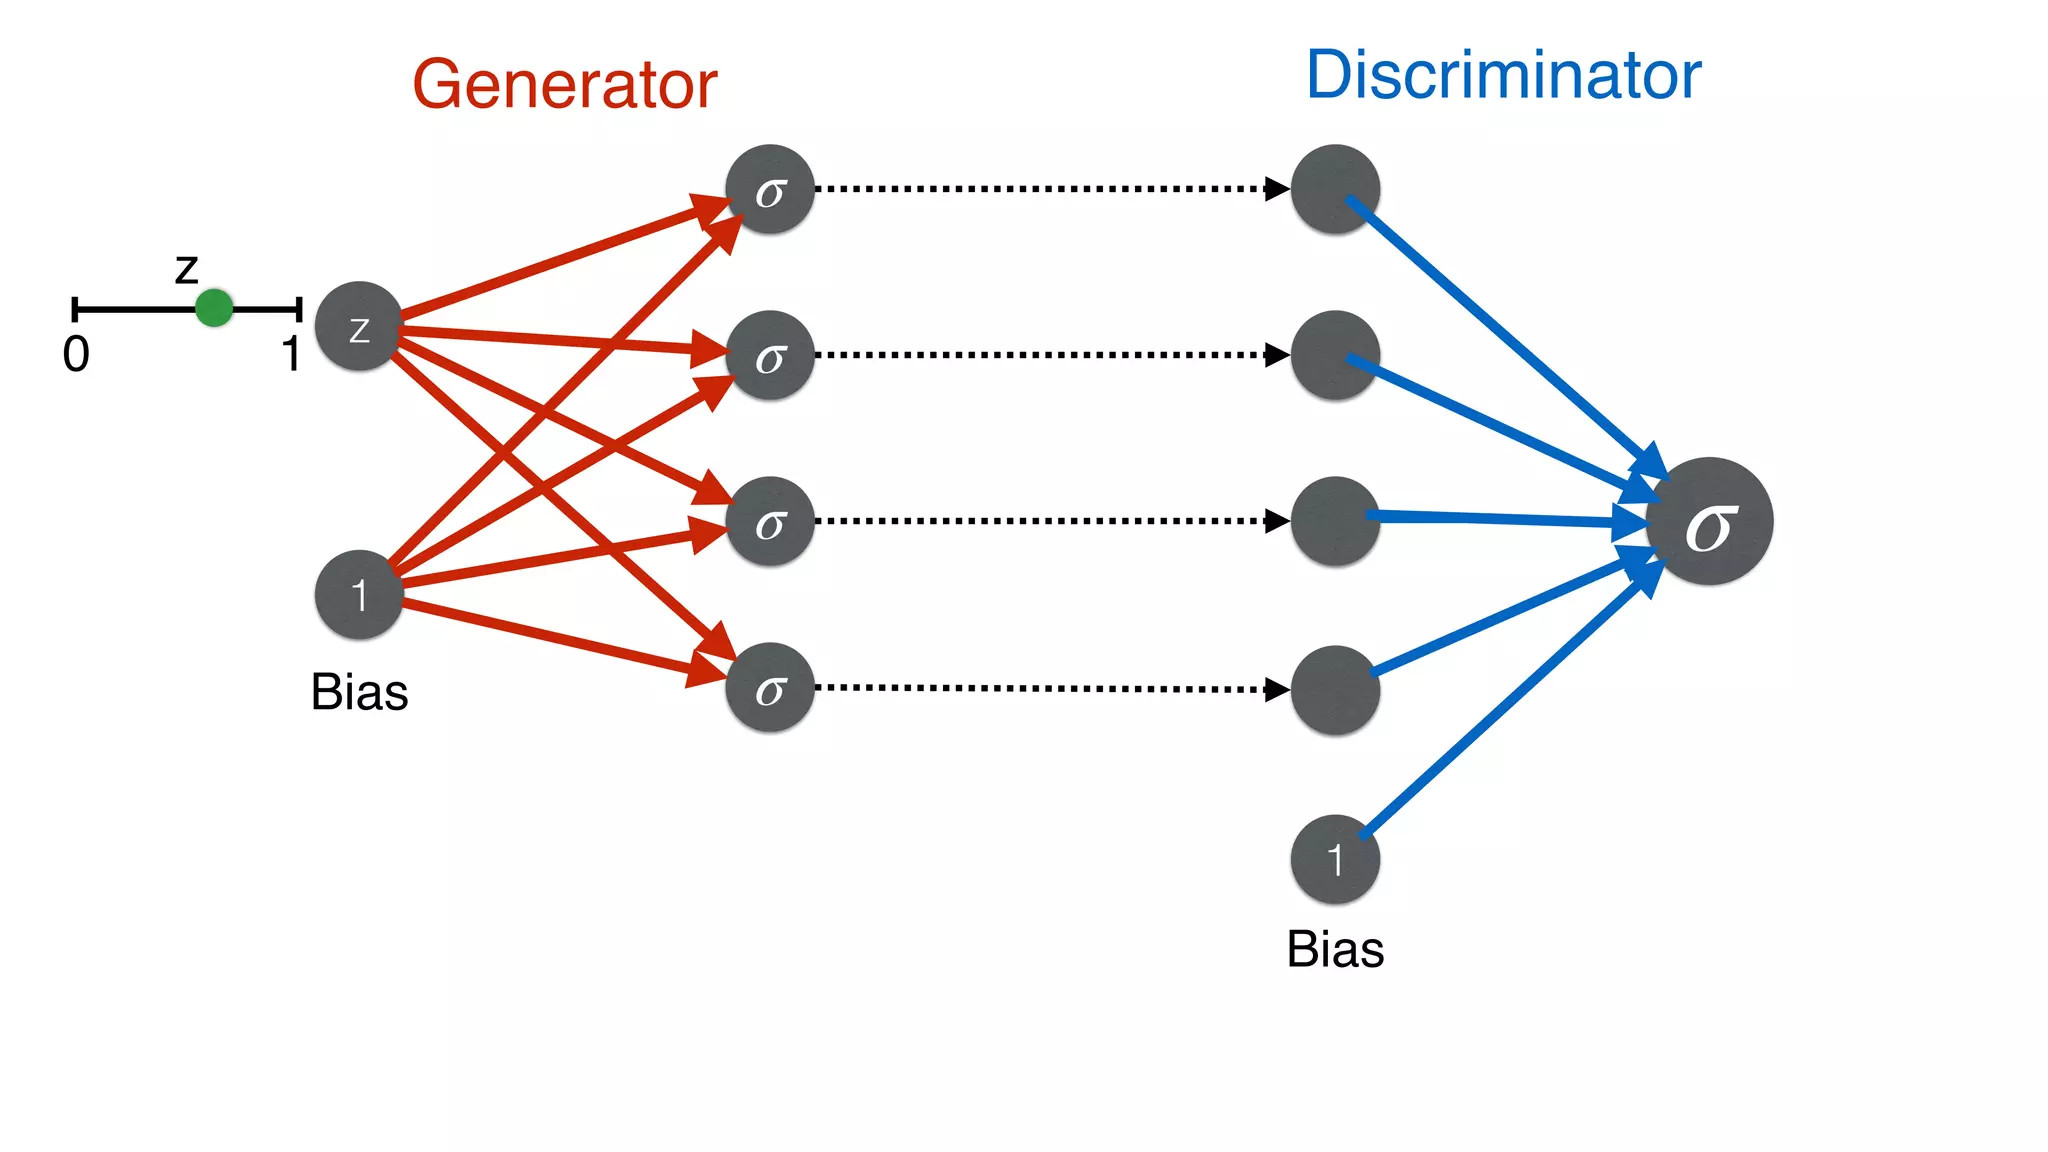
\includegraphics[width=1\textwidth]{Slanted Land/slide_38.jpg}
        }
        \captionsetup{labelformat=empty}
    \end{figure}   
\end{frame}


\begin{frame}{Results}
    \begin{figure}[h]
    \centering
    \begin{minipage}{0.32\textwidth}
        \centering
        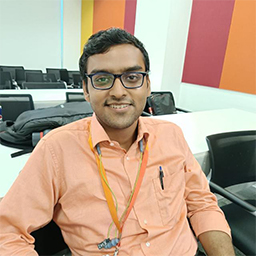
\includegraphics[width=\linewidth]{Image.jpg} % Replace with your image file
        \caption{Original Image of Dwaipayan Haldar}
    \end{minipage}
    \hfill
    \begin{minipage}{0.32\textwidth}
        \centering
        \includegraphics[width=\linewidth]{Image_for_ts_gpt.png} % Replace with your image file
        \caption{Image Distorted by Manas Sarkar}
    \end{minipage}
    \hfill
    \begin{minipage}{0.32\textwidth}
        \centering
        \includegraphics[width=\linewidth]{out_image.jpg} % Replace with your image file
        \caption{Output Image of Dwaipayan Haldar restored by GAN}
    \end{minipage}
\end{figure}
    
\end{frame}

\begin{frame}{Results}
    \begin{figure}[h]
    \centering
    \begin{minipage}{0.32\textwidth}
        \centering
        \includegraphics[width=\linewidth]{Image_ghibli.jpg} % Replace with your image file
        \caption{Original Ghibli Image of Dwaipayan Haldar}
    \end{minipage}
    \hfill
    \begin{minipage}{0.32\textwidth}
        \centering
        \includegraphics[width=\linewidth]{Image_ghibli_Pramit.png} % Replace with your image file
        \caption{Ghibli Image Distorted by Pramit Khamrui}
    \end{minipage}
    \hfill
    \begin{minipage}{0.32\textwidth}
        \centering
        \includegraphics[width=\linewidth]{out_Image_ghibli.jpg} % Replace with your image file
        \caption{Output Ghibli Image of Dwaipayan Haldar restored by GAN}
    \end{minipage}
\end{figure}
    
\end{frame}



% Conclusion slide
\section{Conclusion}

\begin{frame}{}
    \centering
    \Huge{Conclusion}
\end{frame}

\section{References}

\begin{frame}{References}
\scriptsize
    \begin{itemize}
            \item Jireh Jam, Connah Kendrick, Kevin Walker, Vincent Drouard, Jison Gee-Sern Hsu, Moi Hoon Yap,
A comprehensive review of past and present image inpainting methods,
Computer Vision and Image Understanding,
Volume 203,
2021.
            \item  Efros, A.A., Leung, T.K., 1999. Texture synthesis by non-parametric sampling. In: Iccv.
 IEEE, p. 1033.
    \item Texture Synthesis by Non-parametric Sampling https://people.eecs.berkeley.edu/~efros/research/NPS/alg.html
    \item  Thottam, I., 2015. The Cost of Conservation and Restoration. Art Business News,
 http://artbusinessnews.com/2015/12/the-cost-of-conservation-and-restoration/
 \item  Liu, G., Reda, F.A., Shih, K.J., Wang, T.-C., Tao, A., Catanzaro, B., 2018a. Image
 inpainting for irregular holes using partial convolutions. arXiv preprint arXiv: 1804.07723.
 \item Serrano, L. (2019, November 11). Generative adversarial networks (GANs) [SlideShare presentation]. SlideShare. https://www.slideshare.net/slideshow/generative-adversarial-networks-gans-238846644/238846644
 \item  Criminisi, A., Pérez, P., Toyama, K., 2004. Region filling and object removal by
 exemplar-based image inpainting. IEEE Trans. Image Process. 13 (9), 1200–1212.
        \end{itemize}
        
\end{frame}


\begin{frame}{}
    \centering
    \Huge{Thank You!}
    \vspace{1cm}
    \\ \Large{Questions?}
\end{frame}

\end{document}
